\documentclass[10pt,a4paper]{book}
\usepackage[utf8]{inputenc}

% Page configuration
\usepackage[a4paper,top=30mm,bottom=30mm,inner=40mm,outer=30mm]{geometry}
\usepackage{fancyhdr}

% Font configuration
\usepackage[T1]{fontenc}
\usepackage[sfdefault,scaled=.85]{FiraSans}
\usepackage{newtxsf}
\usepackage{siunitx}

\usepackage{amsmath}

% Used to import graphics as figures
\usepackage{graphicx}
\graphicspath{ {./images/} }

% Used to customize the chapter titles
%Options: Sonny, Lenny, Glenn, Conny, Rejne, Bjarne, Bjornstrup
\usepackage[Bjornstrup]{fncychap}

% Used to customize section titles
\usepackage{titlesec}

% Used to customize tables
\usepackage{array}
\usepackage[table]{xcolor}
\usepackage{longtable}

% Define how sections are represented
\titleformat{\section}
	{\normalfont\Large\bfseries\color{sectionColor}}   % The style of the section title
	{}                             % a prefix
	{0pt}                          % How much space exists between the prefix and the title
	{}    % How the section is represented
\titleformat{\subsection}
	{\normalfont\large\bfseries\color{sectionColor}}   % The style of the section title
	{}                             % a prefix
	{0pt}                          % How much space exists between the prefix and the title
	{}    % How the section is represented

% Some style configuration
\setlength{\parindent}{0pt} % Remove indentation of paragraphs
\definecolor{textColor}{cmyk}{0, 0, 0, 0.90}  % Declare regular text color
\definecolor{sectionColor}{rgb}{0.0, 0.48, 0.46}  % Declare section text color
\definecolor{theoryColor}{RGB}{213, 43, 129}  % Declare section text color
\definecolor{theoryBgColor}{RGB}{255, 245, 245}  % Declare section background color
\definecolor{warningColor}{RGB}{255, 151, 7}  % Declare warning text color
\definecolor{warningBgColor}{RGB}{255, 252, 197}  % Declare warning background color
\color{textColor} % Set default color

% Define an environment for the theory of operation blocks
\newenvironment{theory}[2][h]
{		
	\begin{table*}[#1]
	\centering
	\color{theoryColor}	
	\begin{tabular}{ >{\columncolor{theoryBgColor}} p{0.97\textwidth}}
		\hline\\
		\begin{tabular}{ m{12mm} l }
			
\includegraphics[width=10mm]{icons/theory} & 
			{\bf #2}
		\end{tabular}
		\begin{center}
		\begin{tabular}{ p{0.90\textwidth} }
}
{
	\end{tabular}
	\end{center}
	\\\\\hline
	\rowcolor{white}\\
	\end{tabular} 
	\end{table*}
}

% Define an environment for the warning messages
\newenvironment{warning}[1][Warning!]
{	
	\color{warningColor}
	\begin{tabular}{ >{\columncolor{warningBgColor}} p{0.95\textwidth}}
		\hline\\
		\begin{tabular}{ m{12mm} l }
			
\includegraphics[width=10mm]{icons/warning} & 
			{\bf #1}
		\end{tabular}\\\\
	}
	{ 
		\\\\\hline
		\rowcolor{white}\\
	\end{tabular} 
}

% Define a command to show an inline theory of operation reference
\newcommand{\toref}[1]{{\bf \color{theoryColor}	#1}
\includegraphics[width=3.6mm]{icons/theory}}

% Define commands to show symbols
\newcommand{\sym}[1]{{\tt #1}}
\newcommand{\isym}[1]{{\tt $\overline{\mbox{#1}}$}}

% Configure header and footer using fancyhdr package.
\pagestyle{fancy}
\renewcommand{\chaptermark}[1]{\markboth{#1}{#1}}
\fancyhf{}
\fancyhead[LE,RO]{\chaptername\ \thechapter: \leftmark}
\fancyfoot[LE,RO]{\thepage}

\author{Alvaro Polo}
\title{Artemisa Computer Model 101 Technical Handbook}

\begin{document}

\maketitle

\chapter{Introduction}

Welcome to the early days of home computing.

Let me propose a journey to the 80s of the past century. During that decade, the computing industry experienced a big revolution. The lessons learned during the 70s revealed a future where computers domain everything. A future in which computers are everywhere: in the business, in the offices, in the industries... and of course, in our homes.

In these days, many companies produced home computers. That is the age of the Spectrum ZX, the Commodore 64, the Amstrad CPC, and of course the big family of MSX computers. Microcomputers with limited capacity and resources  found their place in our homes when we were just kids. We learned to play video-games with these early computers. We learned to code with them. We learned their potential. Their power to change the modern economies, to transform the World. And we learned all that was just the beginning.

Again, welcome to the early days of home computing. Welcome to Artemisa.

\section{What is Artemisa}

Artemisa is an 8-bit computer system that conforms the MSX-1 specification. There were many hardware vendors that produced MSX computers in the 80s. Sony, Canon, Casio, Sharp, Spectravideo, Panasonic, Philips, ... Artemisa is just another member of this big family, with some particularities.

One of these particularities is that the design of the Artemisa started in 2018. That is 35 years after the initial design of the first MSX computers. But actually this is  not new. In 2006, ESE Artists’ Factory designed the 1chipMSX. This is a FPGA-based computer system that implements the MSX-2 standard. In 2013, a Korean team of MSX enthusiasts known as Retroteam Neo created the Zemmix Neo as an evolution of the 1chipMSX design with inspiration from the classic Zemmix game console produced by Daewoo. Since then, many other teams along the globe had produced their own customizations of Zemmix Neo. Also, in 2020 a group of Spanish makers released the MSXVR. This is an enhanced MSX emulated by a Raspberry Pi with the physical appearance of a classic 8-bit computer.

So yes, Artemisa is just another member that joins the club of MSX computers designed in 21st century. But here comes another particularity. Artemisa is one of the few, along the Omega MSX, that do not use emulation techniques. Some other products as 1chipMSX or Zemmix Neo use FPGAs to emulate the whole MSX hardware. Some others as the MSXVR or the Zemmix Mini uses software emulation on top of an ARM-based computer. In contrast, Artemisa (and Omega) use real integrated circuits and discrete logic. In other words, it is made using the same design techniques and materials used in the 80s, when the first MSX computers were also designed. For example, the heart of the Artemisa computer is a real Zilog Z80 microprocessor instead of a Z80 CPU reimplemented in an HDL language by reverse engineering and synthetized in an Altera Cyclone FPGA.

Please note this does not mean Artemisa is better (or worse) than its FPGA-based or software-based counterparts. It is likely that all the things you can do with Artemisa can also be done in any other MSX computer system, emulated or not. You will not observe any remarkable additional feature, more speed or more stability. All them are functional MSX computers you can enjoy.

\section{Why Artemisa?}

You might ask why you would need an Artemisa computer considering there are some other options out there. Good question!

One possible answer is that you might find Artemisa computer more authentic. Please note I am not saying it is really more authentic. But just you might feel that. There are some users that specially appreciate the real hardware. And they feel more comfortable using an MSX computer that uses the classic technologies, implemented with a real CPU, real VDP, real PSG, real memory, … A computer that is designed using the old-school techniques with bare metal. In contrast, some other users do not care. They do not have a different experience using an emulator than using a traditional computer. If you think you belong to the former group of users, you will enjoy Artemisa. 

In the case of Artemisa Homebrew DIY series, there is another reason for choosing it. You have the chance to learn how an MSX computer is designed from the top to the bottom. And I am not just saying that because you will have to assemble it. Thanks to this book, you will also have the chance to understand how every single chip works. You have access to the schematic designs of every single circuit and an educational guide about their role and operation in the circuit. This is a complete lecture about the architecture and design of MSX computers. A book that will put in your hands the tools to understand how a microcomputer works from the top to the bottom. If you are interested in computer architectures beyond the theory, you will find Artemisa was made for your needs. 

In summary, there we have two good reasons to choose Artemisa: 
\begin{itemize}
	\item Because you feel the real hardware is particularly sexy.
	\item Because you want to learn how an MSX computer works.
\end{itemize}

However, if you only want to have an MSX machine that just works and you are not particularly interested in any of these value propositions, probably other options are better. On one hand, a refurbished MSX or a new FPGA-based one are likely less expensive. On the other hand, some other homebrew designs such as the Omega are more powerful and MSX2-compliant, but they lack the extensive documentation to understand their design. The offer of Artemisa is educative. The goal is to make you learn computer architecture and design at the same time you build and assemble your own MSX computer using real hardware, chip by chip. 

The decision is up to you.

\section{About this document}

As stated above, this handbook compiles all the technical knowledge about the Artemisa Homebrew DIY Computer series. You will find it useful to assemble the parts of the DIY kit. But also, to understand how an MSX computer works in detail. From the smaller chip to its most complex circuit. 

\section{Intended audience}

If you have purchased an Artemisa Homebrew DIY Computer series, you are likely an electronic hobbyist or an MSX fan and you feel skilled enough to assemble a computer system by your own. This means soldering the components following the detailed instructions you will find in this book. 

The Artemisa model 101 is built using electronic components that use large through-hole packages. The integrated circuits used in the design are DIP (Dual Inline Package), with a pad separation of 2.54mm. Other components such as resistors and capacitors are also large. In general, small and space-saving packaging such as SMD (Surface Mount Device) are avoided. This not only resembles the design style of early 80s computers but also lowers the entrance barrier for those that do not trust their own soldering skills. The grade of difficulty of assembling an Artemisa computer model 101 is quite low. 

Thus, only a basic knowledge in soldering is required. If unsure, there are tons of guides in the Internet and hundreds of YouTube tutorials available online to learn how. Assembling this kind of electronic components is easy. Just forget your fears and enjoy the experience!

Also, if you want to take advantage of the educational opportunities of this book, some basic knowledge of computing and digital systems is required. The user is assumed to understand basic concepts such as bit, byte, memory address, bus, CPU, peripheral, logic gate, voltage level, etc. A degree in Computer Science is useful, but not necessary. However, you will make the most from this book if your knowledge is above the standard knowledge of a regular computer user.

\section{How to Read This Book}

There are some parts of the book that have a special meaning or must be read in some specific way. They are described in this section. 

\subsection{Theory of operation blocks}

These blocks will be represented as follows:

\begin{theory}[h!]{Theory of operation}
	Here goes a full detailed description of how a part of the circuit works. 	
\end{theory}

The theory of operation blocks will describe the theory behind a part of the system. A basic knowledge on computing and digital systems is required in order to fully understand these blocks. However, do not worry if you lack this knowledge or find it difficult to understand. This information is not essential to assemble the system. You can still build your Artemisa computer without fully understanding what these text blocks tell. This is just for educational purposes.

When some concept mentioned in the book is related to a theory of operation block, it will be indicated with a book-and-bulb symbol beside. For example, in \toref{this concept}.

\subsection{Warning blocks}

Some operations require special attention to things that, when unnoticed, could cause damage in the circuit. In these cases, a warning text block will indicate you have to pay special attention, like this one:

\begin{warning}[Warning message!]
	This is a warning message that requires your attention.
\end{warning}

\subsection{Schematic diagrams}

Along this document, the different parts of the circuit are explained using schematic diagrams. They are not difficult to understand. But if you are not familiarized at all with them, a brief introduction might be useful. 

Most of the elements you will find in a schematic diagram are shown in Figure \ref{fig:schematic-elements}.

\begin{figure}[h]
	\centering
	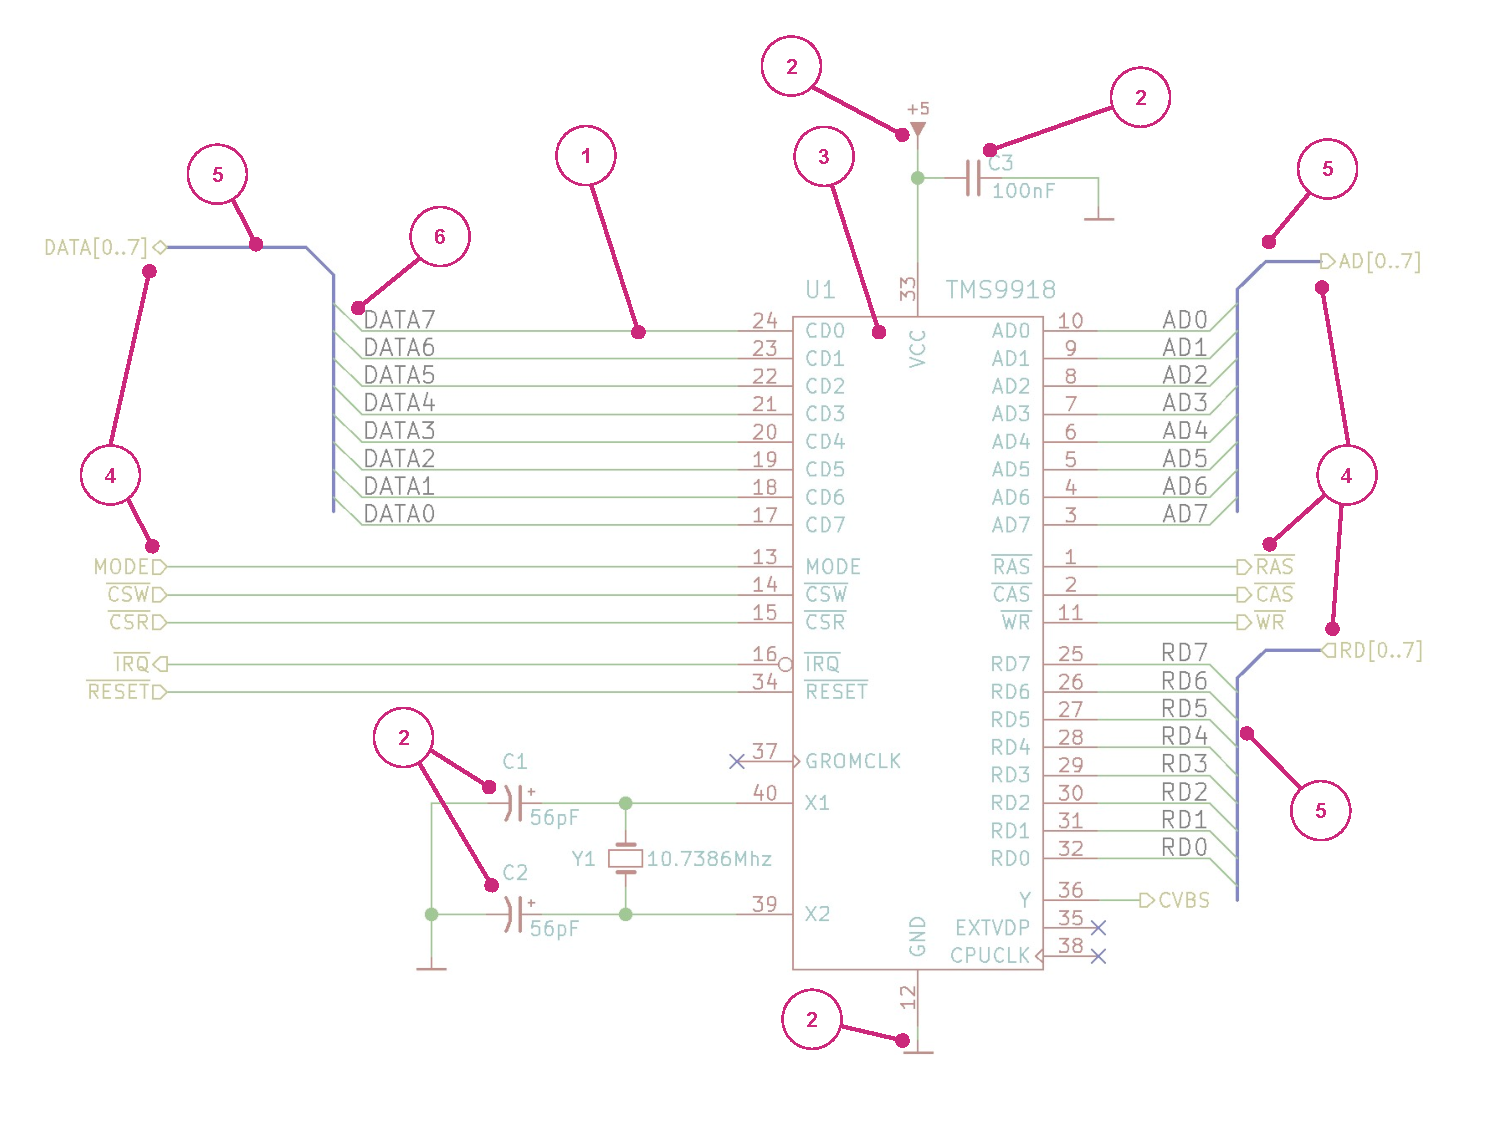
\includegraphics[width=\textwidth]{figures/schematic-elements}
	\caption{Elements of a schematic diagram}
	\label{fig:schematic-elements}
\end{figure}

\begin{enumerate}
	\item Wires. This is the most basic building block of a schematic diagram. It connects two points electrically. This means there will be a copper path between them in the circuit board that will let the current flow among these points.
	\item Basic components. Elements that have one or more pins where wires can be connected. These are power supply terminals, capacitors, resistors, oscillators, logic gates, etc. The different symbols used in this manual are described in Table \ref{table:schematic-symbols}.
	\item Integrated circuits. Components that contain a whole and complex circuit inside it. These are processors, memories, flip-flops, decoders, etc.
	\item Connections from/to other schematic diagrams. The pointing edge indicates the direction of the signal. If it has two pointed edges, it is bidirectional.
	\item Buses. Collections of parallel wires that transmit a multibit data.
	\item Wire connections from/to buses. A label indicates what is the wire that is obtained from the bus.
\end{enumerate}

\begin{table}[h!]
	\centering
	\begin{tabular}{ m{25mm}|l }
		\centering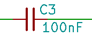
\includegraphics{icons/cap-cer}  & Ceramic capacitor      \\
		\centering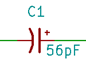
\includegraphics{icons/cap-elec} & Electrolytic capacitor \\
		\centering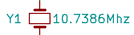
\includegraphics{icons/osci}     & Clock oscillator       \\
		\centering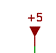
\includegraphics{icons/volt-5}   & 5 volts power supply   \\
		\centering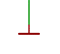
\includegraphics{icons/volt-gnd} & Ground power supply    \\
		\centering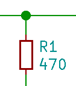
\includegraphics{icons/res}      & Resistor               \\
		\centering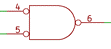
\includegraphics{icons/gate-and} & AND logic gate         \\
		\centering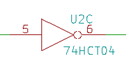
\includegraphics{icons/gate-inv} & Inverter logic gate    \\
	\end{tabular}
	\caption{Component symbols in schematic diagrams}
	\label{table:schematic-symbols}
\end{table}

If you still do not know what a bus, a capacitor or a logic gate is, do not panic. Most of these concepts will be elaborated in the following chapters.

\subsection{Schematic sheets}

TBD

\subsection{Multipart integrated circuits}

Some integrated circuits contain multiple parts under the same chip. Independent elements that operate separately but are encapsulated together. This is the case of most logic gates and many other logic functions such as encoders, decoders, multiplexers, etc. For example, the well known 7404 chip contains six logic inverters, each one using one input pin and one output pin. That is why it is known as an hex logic inverter. The same happens to the 7432, the quad 2-input OR gate that contains four independent functions. 

For legibility reasons, it is common to represent these multipart ICs in the schematic diagrams by separating each independent function as if it was a totally independent component. For example, the 7404 logic inverter is not represented as a single schematic component with six input pins and six output pins, but six separated logic gates with one single input and one single output. The main reason to do that is the each independent function is typically used in different parts of the design. For example, one of the inverters of a 7404 chip can be used in the CPU sheet while some other inverter of the same chip is used in the PSG circuit. This simplifies the reading, allowing you to focus on logic functions instead of chip pinout and connectivity. 

When multipart ICs are used in the schematic diagrams, the power pins of the IC {\tt VCC} and {\tt GND} are only represented in the first part of the IC. The reason is that most of the times we will want to add decoupling capacitors to the power pins. If you do not know yet what a coupling capacitor is, do not worry. We will discuss about this later. Just take the idea that power pins will be represented in the first part of the IC.

The figure \ref{fig:schematic-multipart-ics} shows an example of both things. There, the U9 chip is a 74HCU04 hex logic inverter. Here we can see three logic functions: {\tt U9A}, {\tt U9B} and {\tt U9C}. As you can see, the prefix {\tt U9} in all them indicate they belong to the same package, using letter suffixes to differentiate each function. Also, you can see how the power pins are only visible in {\tt U9A} but not in {\tt U9B}. That is because both parts share the same power inputs. The rest of the parts, {\tt U9D}, {\tt U9E} and {\tt U9F} are used in other schematic sheets, and they also do not show the power pins.

\begin{figure}[h]
	\centering
	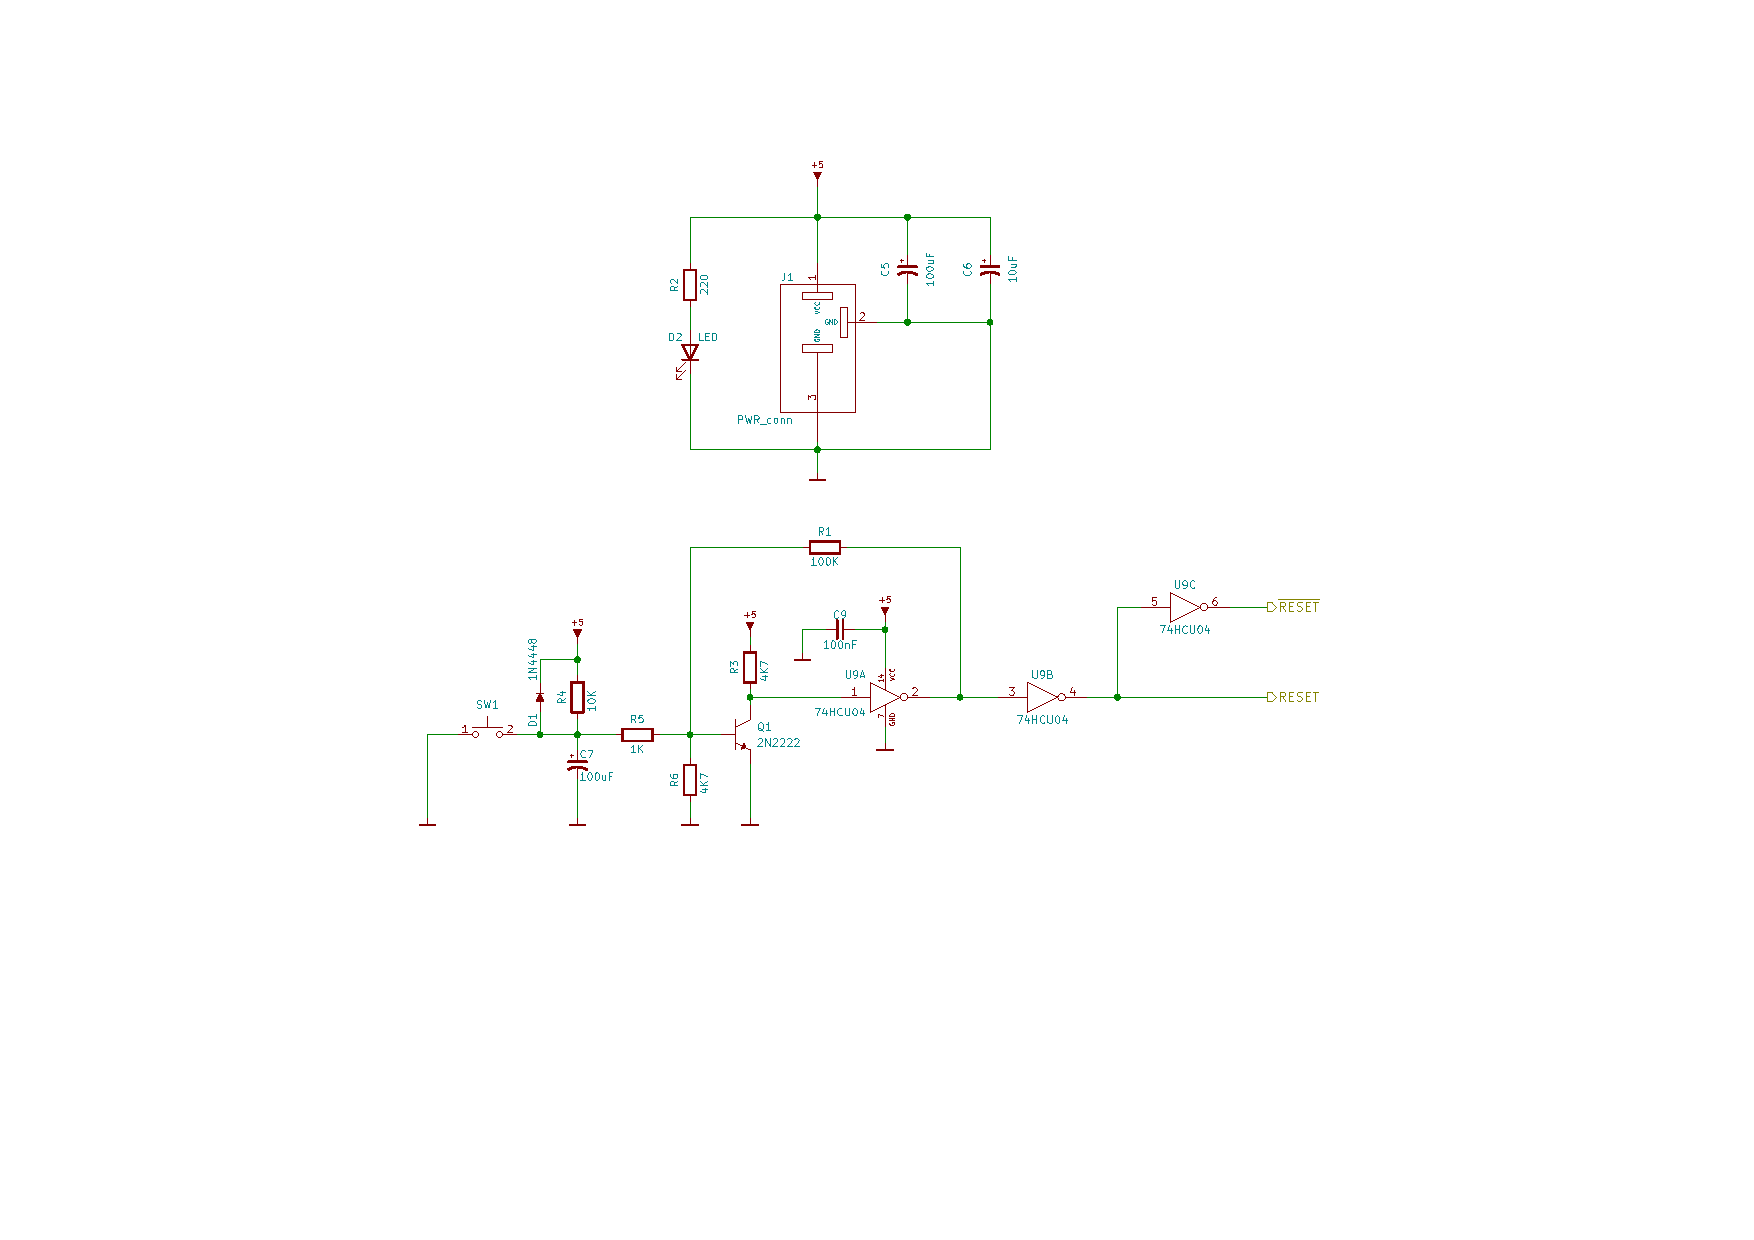
\includegraphics[width=0.7\linewidth,trim={12cm 7cm 8.5cm 8.5cm},clip]{figures/artemisa-schematic-power}
	\caption{Example of a multipart integrated circuit ({\tt U9}) in the schematic diagrams}
	\label{fig:schematic-multipart-ics}
\end{figure}


\subsection{Number notations}

Some numerical values are expressed along this manual. The prefix formats shown in Table \ref{table:number-formats} are used to distinguish between different integer bases. 

\begin{table}[h!]
	\centering
	\begin{tabular}{ r|l }
		{\bf Prefix} & {\bf Description}                               \\
		0b           & Binary number format. Example: 0b01100011.      \\
		0x           & Hexadecimal number format. Example: 0x4A0129FE. \\
	\end{tabular}
	\caption{Number format prefixes}
	\label{table:number-formats}
\end{table}

\chapter{MSX System Architecture}

\section{Overview of an MSX computer}

We can start this book providing a bird’s sight of how an MSX computer is made. It might be obvious, but you will have to understand how an MSX computer works at its highest level before understanding how an Artemisa computer is designed.

Most 8-bit microcomputers are amazingly simple. They include a CPU, a few tens of kilobytes of memory and some peripherals. All of them connected through a \toref{system bus}, as shown in Figure \ref{fig:msx-arch-overview}

\begin{figure}
	\centering
	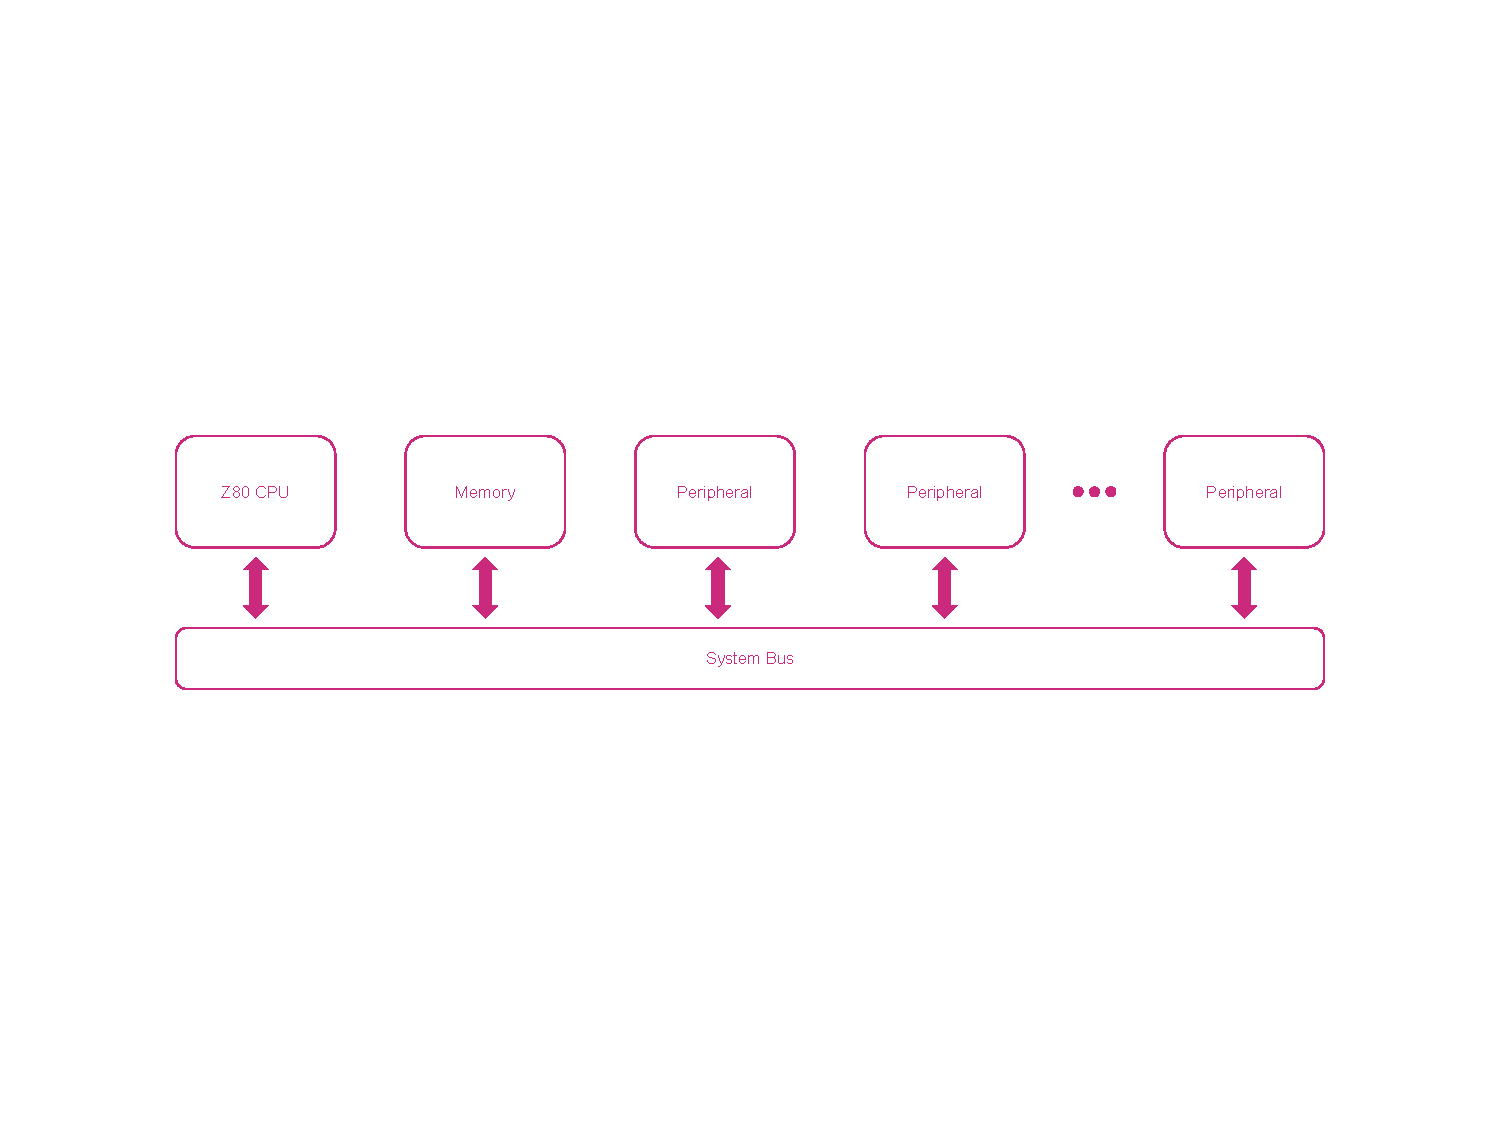
\includegraphics[width=\linewidth,trim={0cm 200 0 200}]{images/figures/msx-arch-overview}
	\caption{High level architecture of a MSX computer}
	\label{fig:msx-arch-overview}
\end{figure}

\begin{theory}{Electronic buses}
	The basic operation of any computer is to move information around. The information is physically represented by electrical wires that may have or not voltage and current. We could simplify this idea by saying that the presence of electrical current and voltage represents the digital number 1, while the absence of it represents the 0. Hence, every single wire can transfer one bit of information at any time.\\\\
	
	A bus in electronics is just a group of wires that have some common purpose. There are some buses that tie the wires together to represent multi-bit magnitudes. For example, if we put 8 wires together, we will have the ability to represent 8-bit numbers. This is a value from 0 to 255 (or -127 to 128). With 16 wires we will represent values from 0 to 65535 (or -32768 to 32767). And so on. Some other times we put wires in the same bus because they represent some information that is closely related. For example, some control signals can be grouped together in the same bus to communicate control actions from one device to another, such as read, write, reset, interrupt, etc.\\\\
	
	If we make an analogy between a computer and the human body, the system bus is the nervous system. In our bodies, it is the medium to transfer the signals from the brain to the muscles to coordinate our actions. But it is also the channel to carry the sensitive information from our five senses to perceive the world. In our computers, the CPU is the brain and the muscles and senses are the peripherals. And all them use the system bus as a kind of nervous system to transfer information in both directions.
\end{theory}

\subsection{The microprocessor}

The CPU of an MSX computer is a Zilog Z80 microprocessor running at 3.58Mhz. The Z80 was introduced by Zilog in 1976 as an enhancement and direct competitor of the popular Intel 8080. It was binary compatible with the Intel CPU, which means it can execute programs originally created for the 8080. Thanks to this and its extended instruction set, it was positioned as one of the most successful CPUs of all the times. It was chosen by Sinclair to make most of their computers, including the top selling ZX Spectrum. It was also the CPU behind the Amstrad CPC series, and some other game consoles such as the ColecoVision and the Sega Master System. And, of course, it is the brain of any MSX computer system. 

\subsection{The memory}

The memory system of an MSX system is comprised by RAM (typically 64KB) and ROM (typically 32KB) memory. The ROM memory is a read-only memory whose content is written during the manufacturing process. It is used to store the \toref{MSX BIOS} and the MSX Basic interpreter. The RAM memory, in contrast, can be read and written. It is used to store the programs that are loaded from storage devices such as the cassette tape or the floppy drive, and to store the data used by these programs. The RAM memory is volatile, which means its contents will be lost after power off or reset. In contrast, the ROM memory is persistent. Once written during the manufacturing process, its contents will persist until the end of the days or until it is destroyed. The thing that happens first.

However, the memory system of the MSX is quite complex. It has a sophisticated bank switching mechanism to break the limit of 64KB of memory space of the Z80 CPU, as we will see later in detail in page \pageref{sec:msx-mem-slots}. Hence, it uses a not trivial decoding and slot selection logic to interpret the signals coming from the system bus and the Parallel Peripheral Interface (PPI) in order to identify the memory device when it is addressed, as shown in Figure \ref{fig:msx-arch-memory}. Do not worry about PPI for now, we will cover this later. 

\begin{theory}{The MSX BIOS}
	BIOS is the acronym of Basic Input/Output System. This is an essential software program present in any computer system that serves two purposes.\\\\
	
	First, it is the first software the CPU will execute upon boot. Thus, it is responsible of preparing the system before the first program can run. Here preparing the system means initializing the hardware into a consistent state, perform a few sanity-checks to ensure the hardware is not malfunctioning and locate the first program that will run. This first program is typically an operating system. In our case, the MSX Basic or the MSX DOS.\\\\
	
	The second purpose is to provide a software abstraction layer over the hardware. The BIOS is a sort of software library that provides utility routines the programmer can use to interact with the hardware. This not only simplifies the life of the programmers, but also ensures the portability of their programs. The BIOS hides the divergencies of the hardware behind an API (Application Programming Interface). So in case of a computer having a different hardware, it is possible to reprogram its BIOS to deal with the differences so that the user software can also run on it without any change.
\end{theory}

\begin{figure}
	\centering
	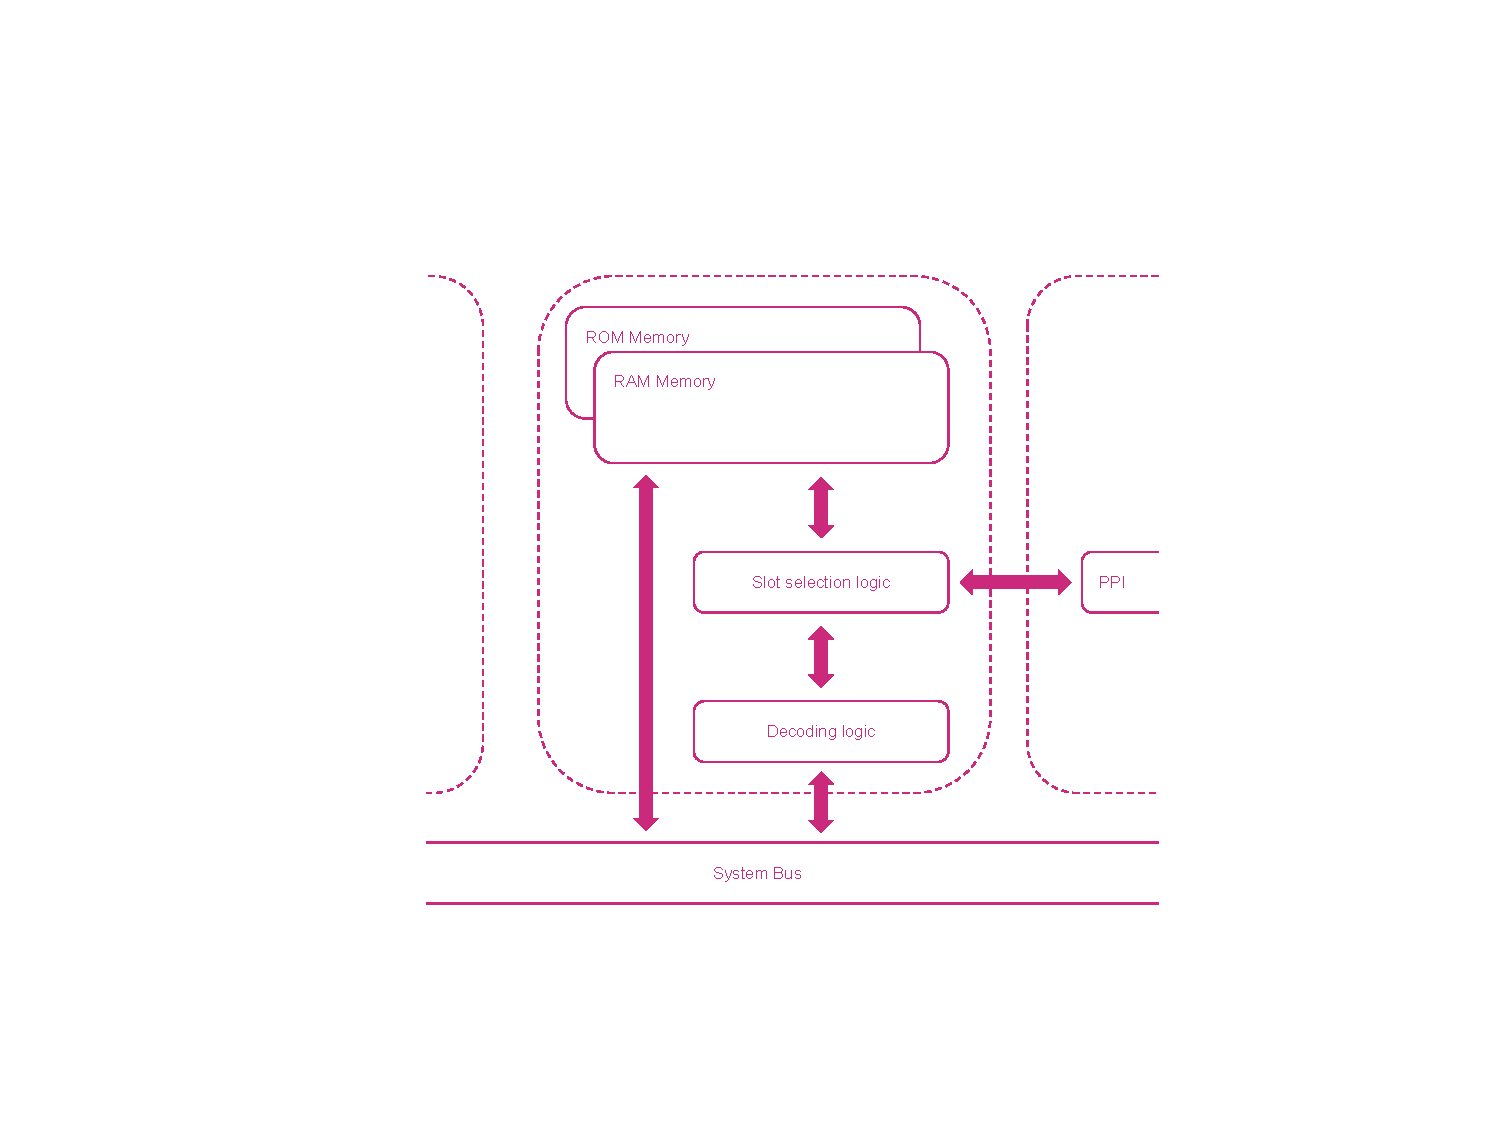
\includegraphics[width=1\linewidth,trim={0cm 100 0 100}]{images/figures/msx-arch-memory}
	\caption{High level architecture of the MSX memory}
	\label{fig:msx-arch-memory}
\end{figure}

\subsection{The Video Display Processor}

If we think about it, a computer made just of CPU and memory is a useless junk that only serves to dissipate heat and contribute to the global warming. It needs some peripherals to interact with the users, receiving data and programs as inputs and showing the result of these programs as outputs. 

Perhaps the most important peripheral is the Video Display Processor (VDP). This is a circuit responsible of producing the video display in the computer. In the MSX standard, this is done by a chip of the Texas Instruments TMS9918 family, as shown in Figure \ref{fig:msx-arch-vdp}. This chip encapsulates all the logic necessary to display images in a TV set or suitable monitor. It is connected to the system bus through a decoding logic to adapt the signals. One of its main particularities is that it uses its own separated video RAM memory to store the images and the sprites it will display in the screen. 

\begin{figure}
	\centering
	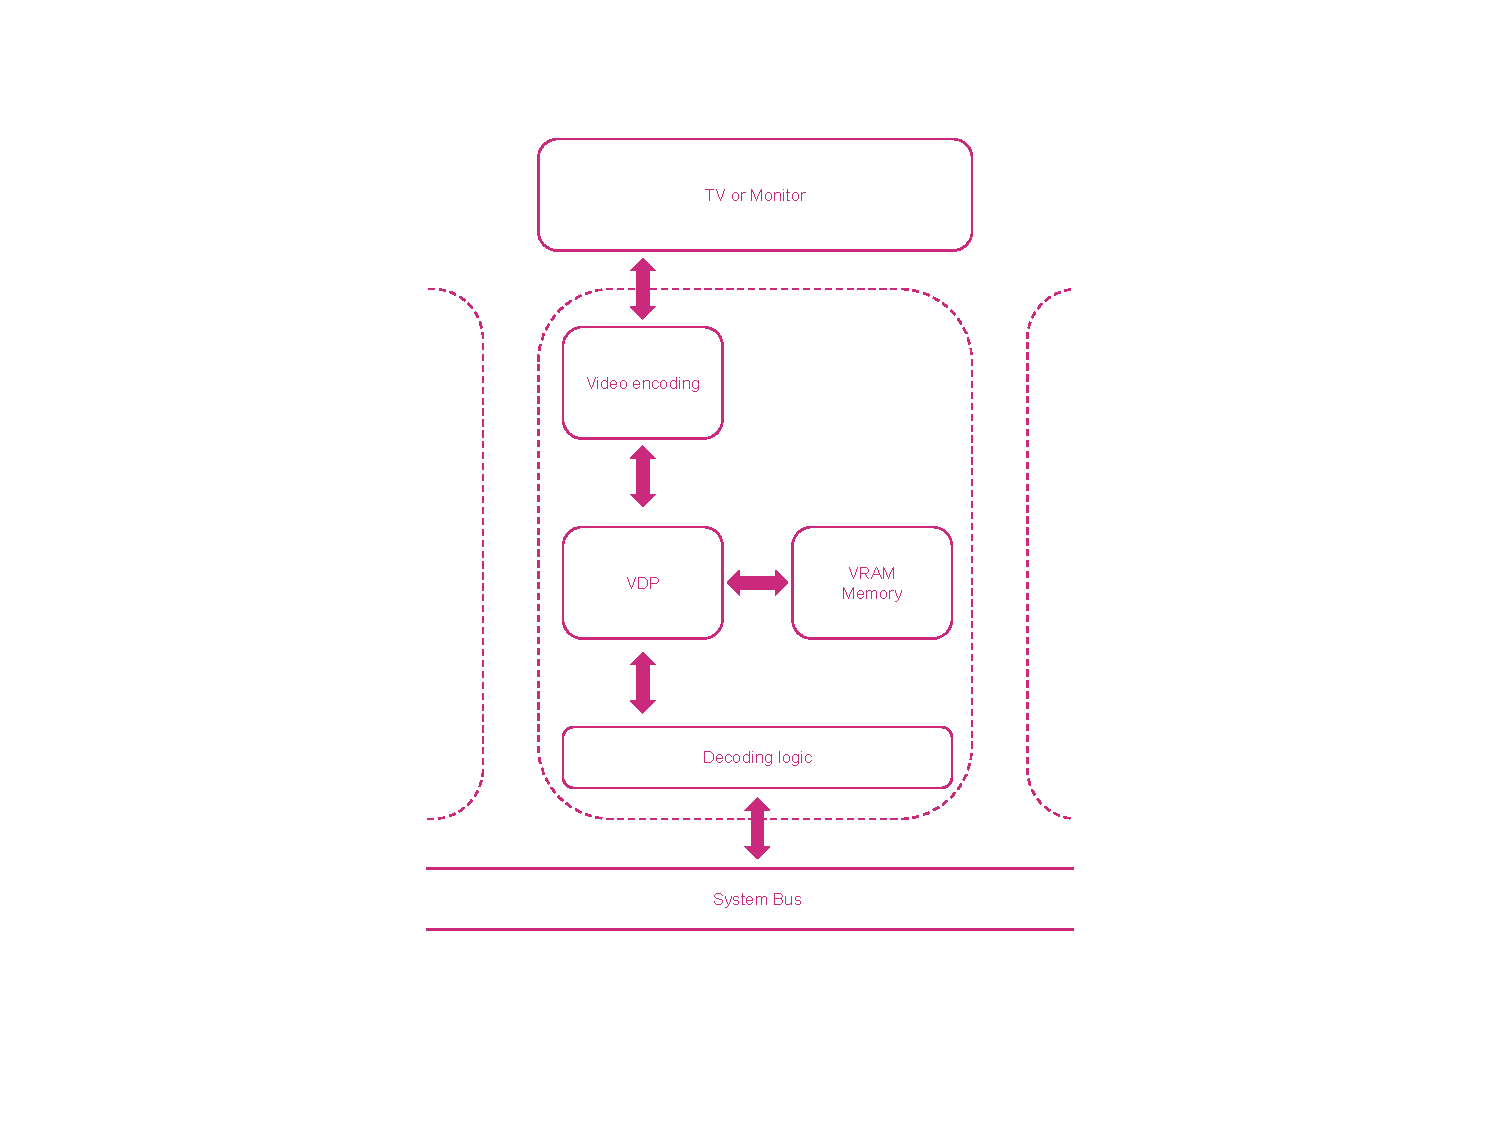
\includegraphics[width=1\linewidth,trim={0cm 100 0 100}]{images/figures/msx-arch-vdp}
	\caption{High level architecture of the MSX Video Display Processor}
	\label{fig:msx-arch-vdp}
\end{figure}

It is worth to remark this particularity of the VDP design in an MSX computer. Almost any other system uses a video display that shares the RAM memory with the CPU. The computer programs must write the data of the images they want to display into a specific section of the main RAM memory. And the display processor will read from that memory area to calculate the pixels that will be shown into the screen. 

As you might think, sharing the memory between two different devices that can potentially access to the same addresses at the same time is not easy. This is known as memory contention. And it is full of tradeoffs. Consider that the video display cannot stop doing its job because the memory is being used by the CPU. If it does, we would observe artifacts in the screen such as flickering images caused by the interruption of the video stream. In some cases, this is addressed by finding the perfect timing on the accesses to the system bus, as Steve Wozniak did for the Apple ][. In some other cases, the CPU is forced to wait when memory contention occurs, losing precious CPU cycles and impacting the system performance. This is the case of the ZX Spectrum and the Amstrad CPC computers. 

In contrast, the MSX computers strictly separates the system RAM from the video RAM. The programs only access the VRAM indirectly by sending \toref{I/O requests} to the VDP to perform read or write operations on the VRAM. The VDP coordinates the access to the memory for both: read the bitmaps to display the screen and process the read or write requests coming from the CPU. The result is a simpler computer architecture without memory contention that do not sacrifice CPU cycles. 

\begin{theory}{I/O requests}
	The Z80 microprocessor, as many others, includes the concept of I/O operations in its design. I/O is just an acronym of Input/Output. The CPUs that embrace this concept implement a specific way to communicate to and from system peripherals by means of an I/O request.\\\\ 
	
	An I/O request is a communication initiated by the CPU whose destination is a specific device attached to the system bus. The request can be one of two types: a read operation to transmit a byte from the device to the CPU, or a write operation to transmit a byte from the CPU to the device. The device that must respond to the request is identified by an 8-bit number known as the I/O port. The CPU uses the signals of the system bus to indicate the start of an I/O request, the port of the device that must respond, and whether it is a read or a write operation. The byte that is exchanged between the CPU and the device is also transferred through the system bus. \\\\
	
	For example, if the CPU wants to write the byte 0xAB to the VRAM address 0x1234, it will have to follow this sequence of I/O requests:
	
	\begin{itemize}
		\item I/O request to port 0x99 to write the byte 0x34. This will tell the VDP the least significant bits of the VRAM address that will be written.
		\item I/O request to port 0x99 to write the byte 0x52. This is the six most significant bits of the VRAM address (0x12) that will be written, prefixed with 0b01. These two bits prefix indicates the VDP must be prepared for a VRAM write operation immediately after.
		\item I/O request to port 0x98 to write the byte 0xAB. This is the byte the VDP will write to VRAM address 0x1234.
	\end{itemize}
	
	Some other CPUs, such as the MOS 6502 or the Motorolla 68000 do not implement the concept of I/O request. These CPUs uses memory access instructions equally to access the memory or access other bus devices. This means part of the memory address space must be  reserved for I/O operations. 	
\end{theory}

\subsection{The parallel peripherals}

Once we can display the results of the programs our MSX computer executes, it is time to think about receiving some inputs. One of the most important pieces used in the MSX architecture to achieve this is the Parallel Peripheral Interface (PPI), shown in Figure \ref{fig:msx-arch-ppi}.

\begin{figure}
	\centering
	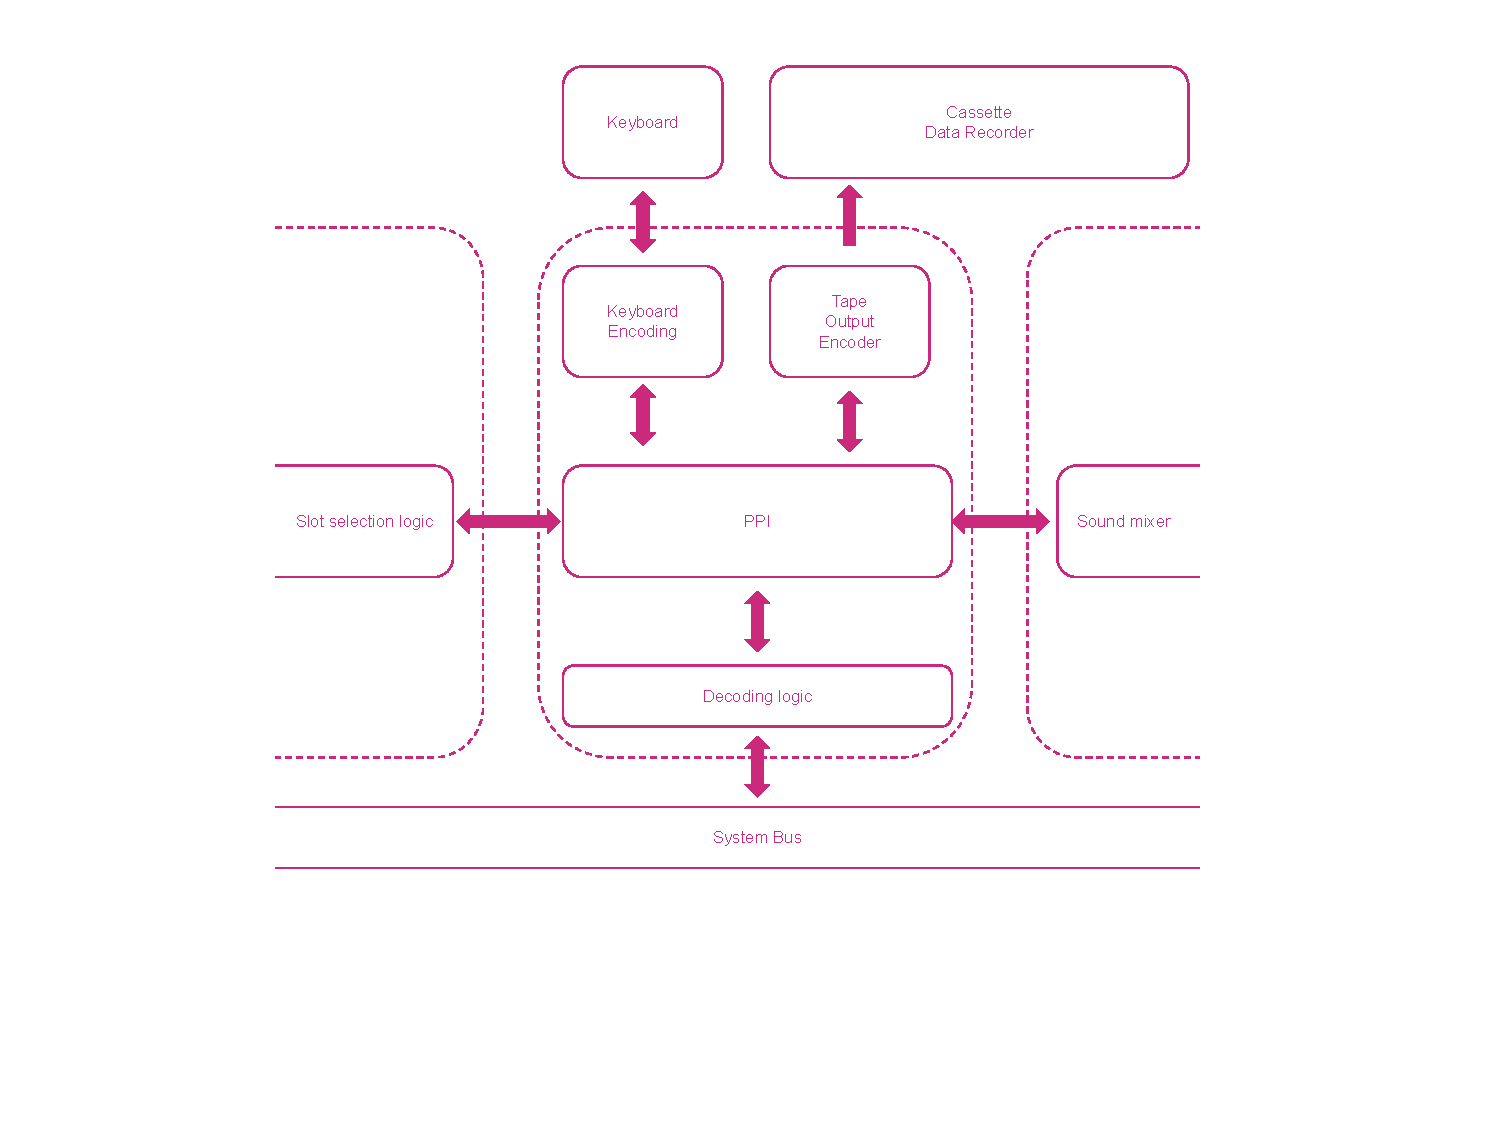
\includegraphics[width=1\linewidth,trim={0cm 100 0 100}]{images/figures/msx-arch-ppi}
	\caption{High level architecture of the MSX Parallel Peripheral Interface}
	\label{fig:msx-arch-ppi}
\end{figure}

The PPI is an Intel 8255 integrated circuit that will act as hardware controller for some peripherals and a few control lines of the system. This is the same chip included in the IBM PC computer, still present in the chipsets of most of modern PC designs. The 8255 has three 8-bit ports: A, B and C. Each port can be configured by software as input or output. The MSX BIOS will configure each port at convenience on system boot. 

The system peripherals that are attached to the system through the PPI are connected by wires to some lines of its three ports, as shown in Figure \ref{fig:msx-arch-ppi-ports}. The mission of this chip in the MSX is to serve as an interface adapter for the peripherals that cannot be directly connected to the system bus, such as the keyboard and the cassette data recorder. Using I/O requests, the CPU can read from the input ports and write to the output ports of the PPI. Which is analogous to read or write from or to the peripherals attached to the ports.

\begin{figure}
	\centering
	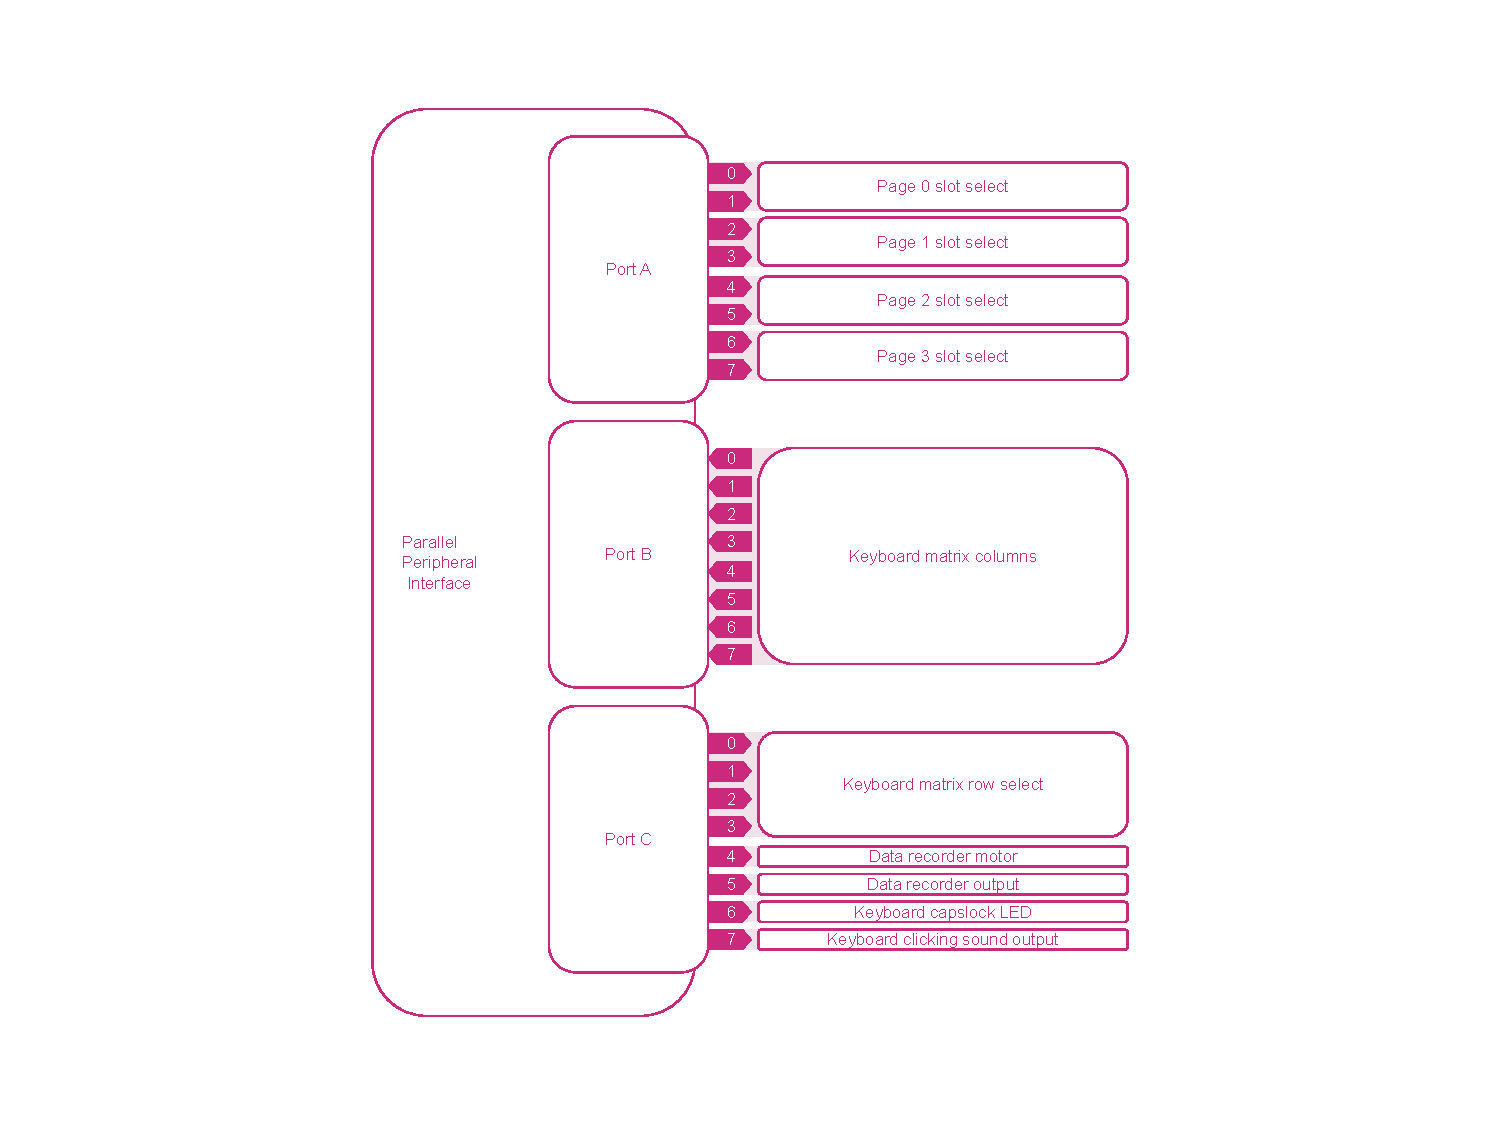
\includegraphics[width=1\linewidth,trim={0cm 50 0 50}]{images/figures/msx-arch-ppi-ports}
	\caption{Ports of the MSX Parallel Peripheral Interface}
	\label{fig:msx-arch-ppi-ports}
\end{figure}

The port A of the PPI is configured by the BIOS as output during the system boot. This port is responsible of choosing the memory slot to be used for every memory page. Each pair of bits determine the primary memory slot of a memory page. Since two bits are used per memory page, we can choose among 4 different primary memory slots. Do not panic if you still do not understand a word about this. It is a complex subject we will cover in detail later. 

The port B of the PPI is configured by the BIOS as input. All eight bits are connected to the columns of the keyboard matrix. The port C is configured as ouput. The four less significant bits are used to select one row of the keyboard during the scanning process. Bits 4 and 5 are used to control the data recorder. Bit 6 is used to drive the LED of the capslock key of the keyboard and bit 7 is used to produce clicking sounds when keys are typed. 

As you can see, the most important peripheral attached to the PPI is the keyboard. This is the time to tell how it works in an MSX computer and the meaning of these rows and columns thing. The keyboard of the MSX is implemented as a X-Y matrix of 8 columns and up to 12 rows, as shown in Figure \ref{fig:msx-arch-kbmatrix}. The total number of rows depends on the keyboard distribution. There is a key switch that connects every row to every column of the matrix. When a key is pressed, the row and the column connected by the switch form a closed circuit. When this happens, any current driven through the wire of the row will propagate to the column. Otherwise, if the key is not pressed, we will have an open circuit and the column will have no current. 

\begin{figure}
	\centering
	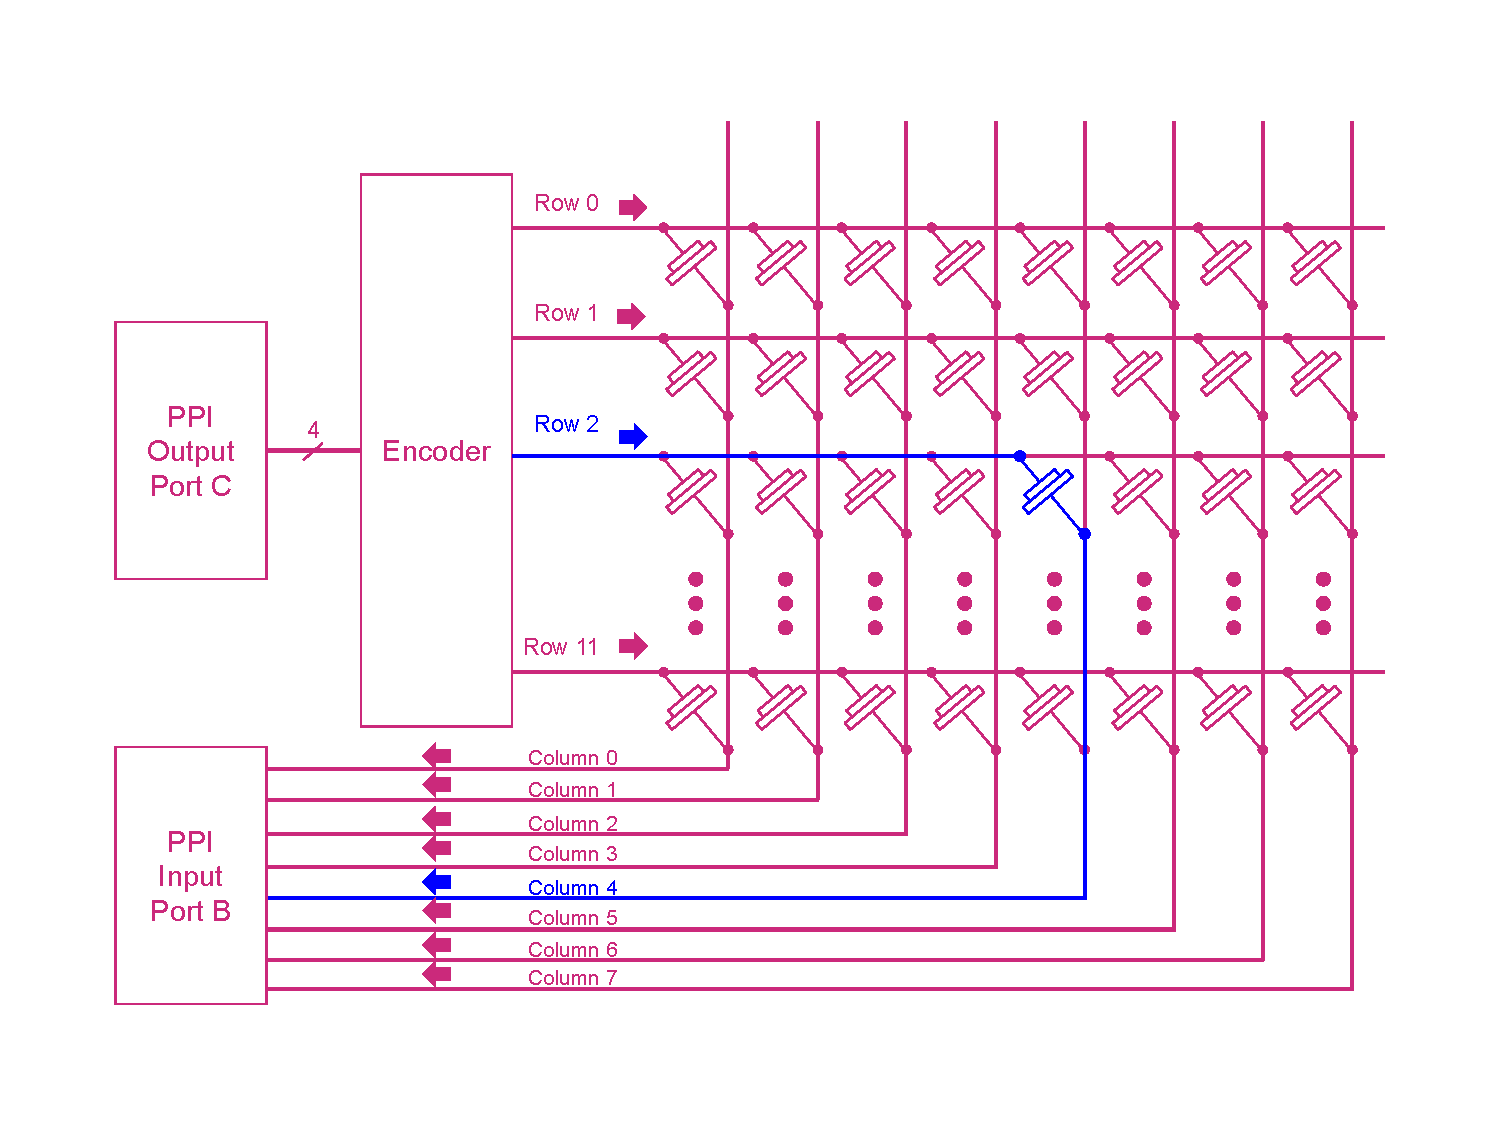
\includegraphics[width=1\linewidth,trim={0cm 5 0 0 40}]{images/figures/msx-arch-kbmatrix}
	\caption{Keyboard matrix of a MSX computer}
	\label{fig:msx-arch-kbmatrix}
\end{figure}

In order to make it work, the MSX uses the PPI to drive the row signals of the matrix and read the status of the columns.  The four less significant bits of output port C of the PPI are used to encode the row that will drive the current. And the whole eight bits of input port B are connected to the matrix columns. The system software, typically the BIOS, will scan the matrix periodically. On each scan, it will loop from the first to the last row. In each loop iteration, it will select the i-th matrix row and read the status of the 8 columns. The row can be selected by writing its 4-bit number in the corresponding bits of the port C of the PPI through an I/O request. The columns can be checked by reading the port B of the PPI through an I/O request. If that read of port C reveals the current is driven in the j-th column, it means the key located at i-th row and j-th column in the matrix is pressed. Otherwise, it is depressed. 

The bit 6 of PPI port C is also involved in the keyboard operation. It drives the LED of the capslock key. As you might think, this is controlled by software. It can be turned on and off by setting 0 and 1 in that bit of port C, respectively. 

The bits 4 and 5 of the PPI port C are connected to the cassette data recorder. The data recorder is an unexpensive storage device that uses cassette tapes to transmit information to and from the computer. It is a cassette player that reproduces the sounds from the tape when reading and records the sound signal on the tape when writing. The sound signals encode binary data in a special kind of frequency modulation known as FSK (Frequency-Shift Keying) following the Kansas City standard. This norm establishes that a “0” bit is encoded by one wave cycle at a frequency of 1200 Hz. While a “1” bit is encoded by two cycles of a 2400 Hz wave. The sound wave reproduces a sequence of beeps alternating between 1200 and 2400 Hz, which in fact represents zeroes and ones that are transmitted from or to the computer. 

In the MSX, all this encoding is generated by software. The bit 5 of the PPI port C is used to generate a squared waveform when writing a file to the data recorder. This is made typically by the MSX BIOS by writing zeroes and ones in that bit of the PPI port one by one. Fortunately, this FSK encoding system operates at low frequencies, below 4800 Hz in the worst case. The Z80 processor at 3.58Mhz can write these sequences of bits fast enough to ensure the waveform is well formed. 

The wave generated through bit 5 of PPI port C is squared because the signals of the PPI ports are digital. Thus, they can only generate +5 and 0 voltage levels, as shown in Figure \ref{fig:msx-arch-fskenc}. There is a tape output encoding circuit that transforms this squared wave into a sinusoidal waveform. Which is what the data recorder expects from the computer. The process to read a file is similar. But it involves other peripherals we will cover soon.

\begin{figure}
	\centering
	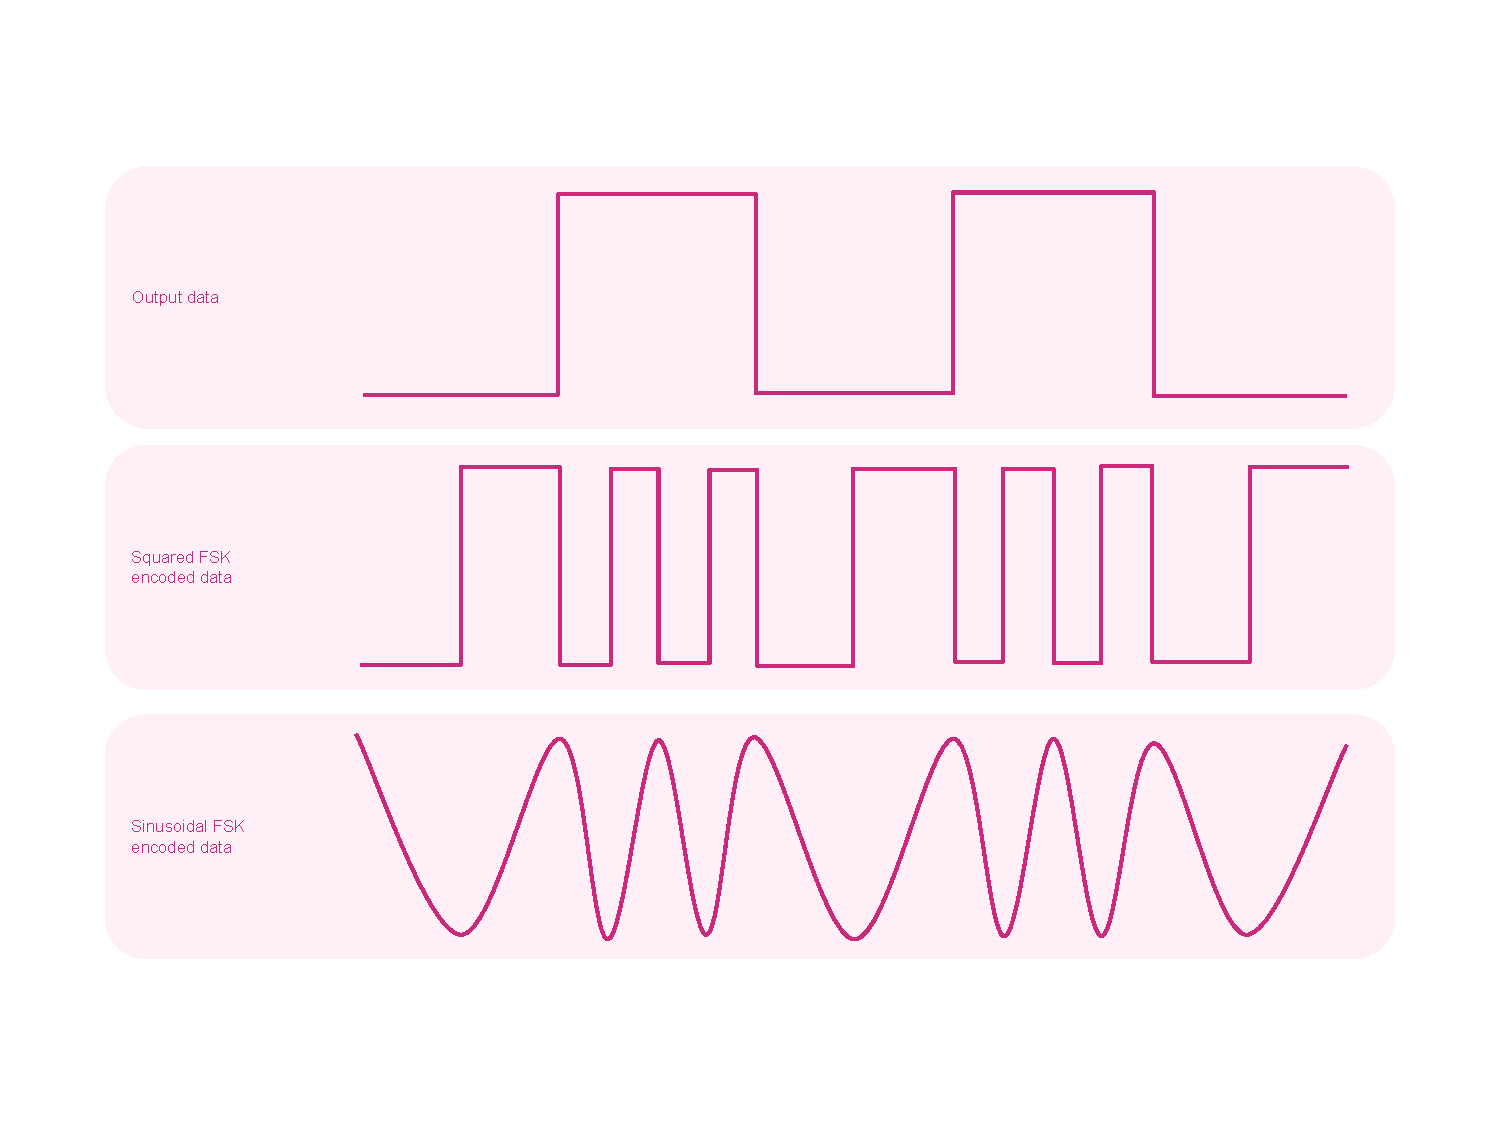
\includegraphics[width=1\linewidth,trim={0cm 80 0 80}]{images/figures/msx-arch-fskenc}
	\caption{FSK encoding in the MSX data recorder}
	\label{fig:msx-arch-fskenc}
\end{figure}

\subsection{Programmable Sound Generator}

A computer without a sound system is like a garden without flowers. And we already know the MSX is one of the best in its category. Of course, it has a programmable sound generator to play sounds and music. 

This is implemented by the General Instrument AY-3-8910. This is a chip that can generate three independent sound channels programmed by software. It was released in 1978 and used in innumerable arcade machines and microcomputers. Including the ZX Spectrum, the Amstrad CPC and the Apple ][. 

The 8910 is attached to the system bus of the MSX through a decoding logic to adapt its interface, as shown in Figure \ref{fig:msx-arch-psg}. Such interface give access to three different I/O ports: the address port, the data write port and the data read port. 

\begin{figure}
	\centering
	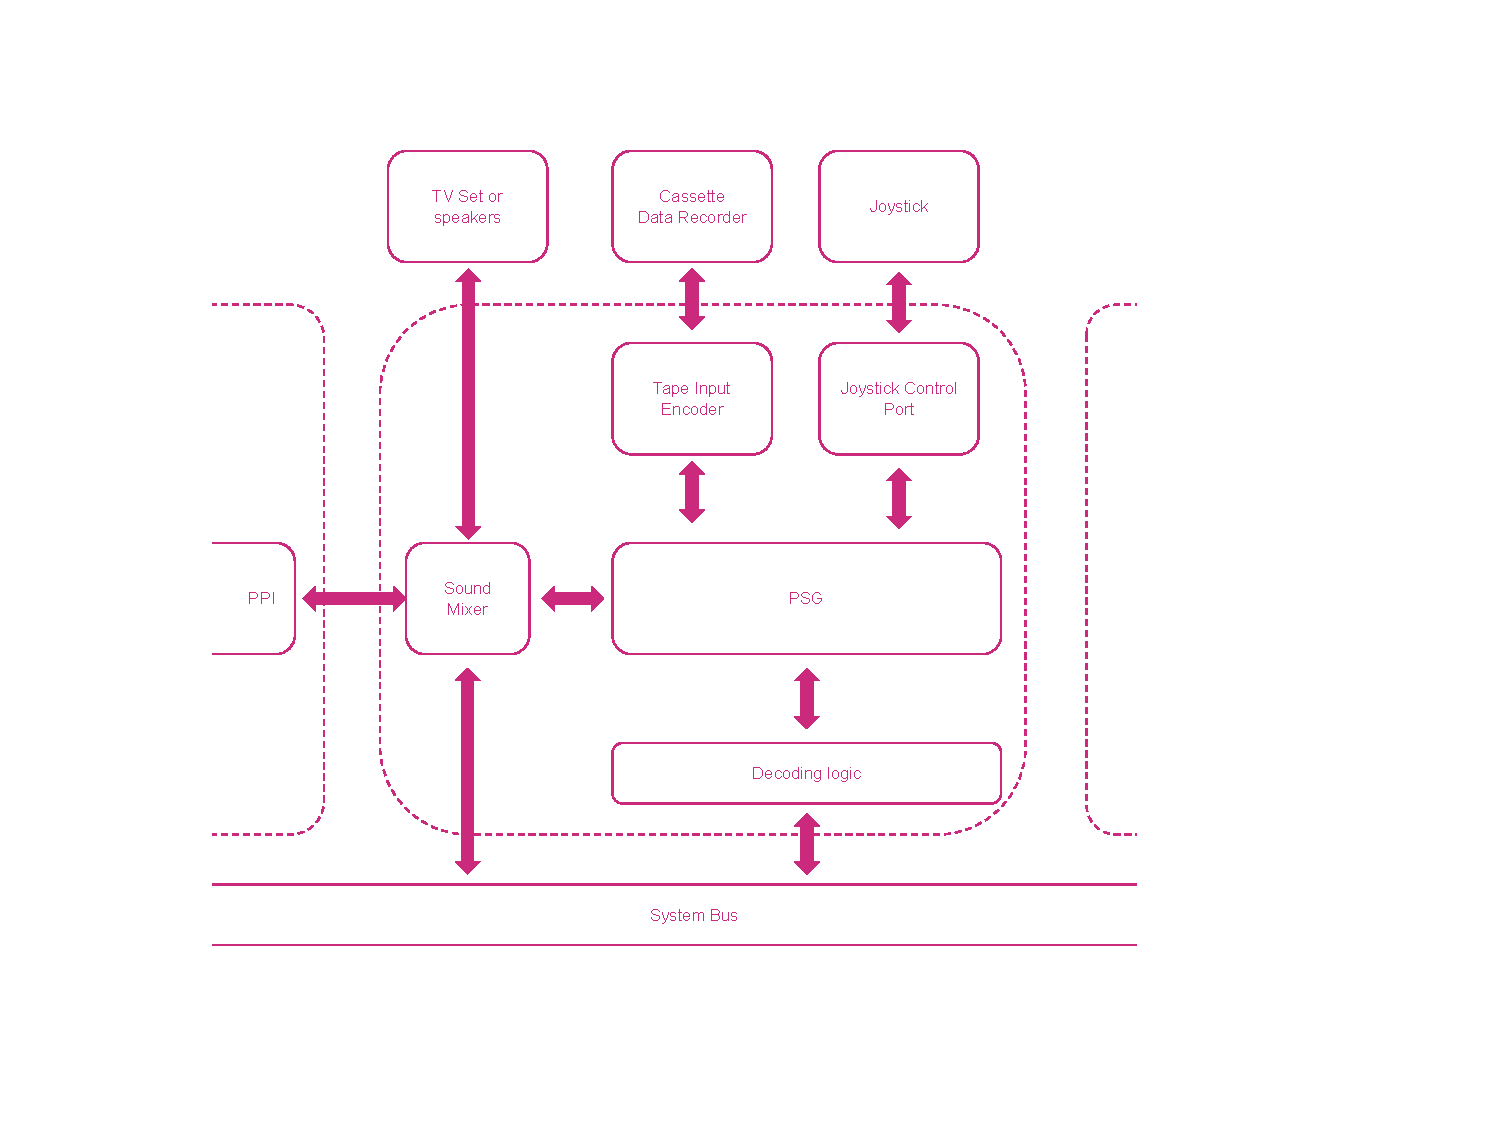
\includegraphics[width=1\linewidth,trim={0cm 80 0 50}]{images/figures/msx-arch-psg}
	\caption{High level architecture of the Programmable Sound Generator}
	\label{fig:msx-arch-psg}
\end{figure}

The address port is used to indicate the address of the internal register that will be read or written. The PSG has 16 internal registers numbered from 0 to 15. Writing the PSG register number in I/O port 0xA0 will prepare the chip to use that register in subsequent read or write operations.

The PSG data write port is available at I/O port 0xA1. This port is used to write bytes to the PSG register that was addressed by previous writes to 0xA0. The PSG data read port at 0xA2 does the same for reading. 

Using these three ports, the system software can program the PSG to generate sounds. As said above, the PSG has three independent channels that can generate separated sounds. However, the MSX was designed in a time when the mono sound was the standard. Thus, the common choice of all MSX computers is to mix the three channels into a single sound signal. This is done by a sound mixer circuit. The mixer also receives the inputs from other devices that are also part of the final sound signal sent to the TV set or the speakers, as shown in Figure \ref{fig:msx-arch-psg}. 

If you remember the Figure \ref{fig:msx-arch-ppi-ports}, the bit 7 of PPI port C is used to produce the characteristic click sound when the user types in the keyboard. This sounds comes from a rudimentary squared waveform produced by this bit from the PPI. The system software, typically the BIOS, will write an alternating sequence of zeroes and ones to this bit of the PPI port C that produces the squared wave. The port bit is connected to the sound mixer to include it in the sound signal that goes to the TV set or the speakers. 

Finally, there is another input that feeds the sound mixer. It is the sound signal coming from the system bus. As we will see soon, the MSX is designed to be expandable. And to take this idea to the top, the external expansion devices can produce their own sound signal that will be mixed with those produced by the PSG and the keyboard clicks. Thanks to this, the PSG can be complemented with another sound chips connected through the expansion slots. 

That is all concerning sound generation. However, the AY-3-8910 was designed to assume other tasks in the system. It also incorporates two I/O ports that can be used to connect parallel peripherals in a similar way as we do with the PPI. These ports are named A and B. They can be programmed as input or output. And in MSX, they are used to connect the general-purpose ports, the data recorder input and a few other IO/functions as shown in Figure \ref{fig:msx-arch-psg-ports}. 

\begin{figure}
	\centering
	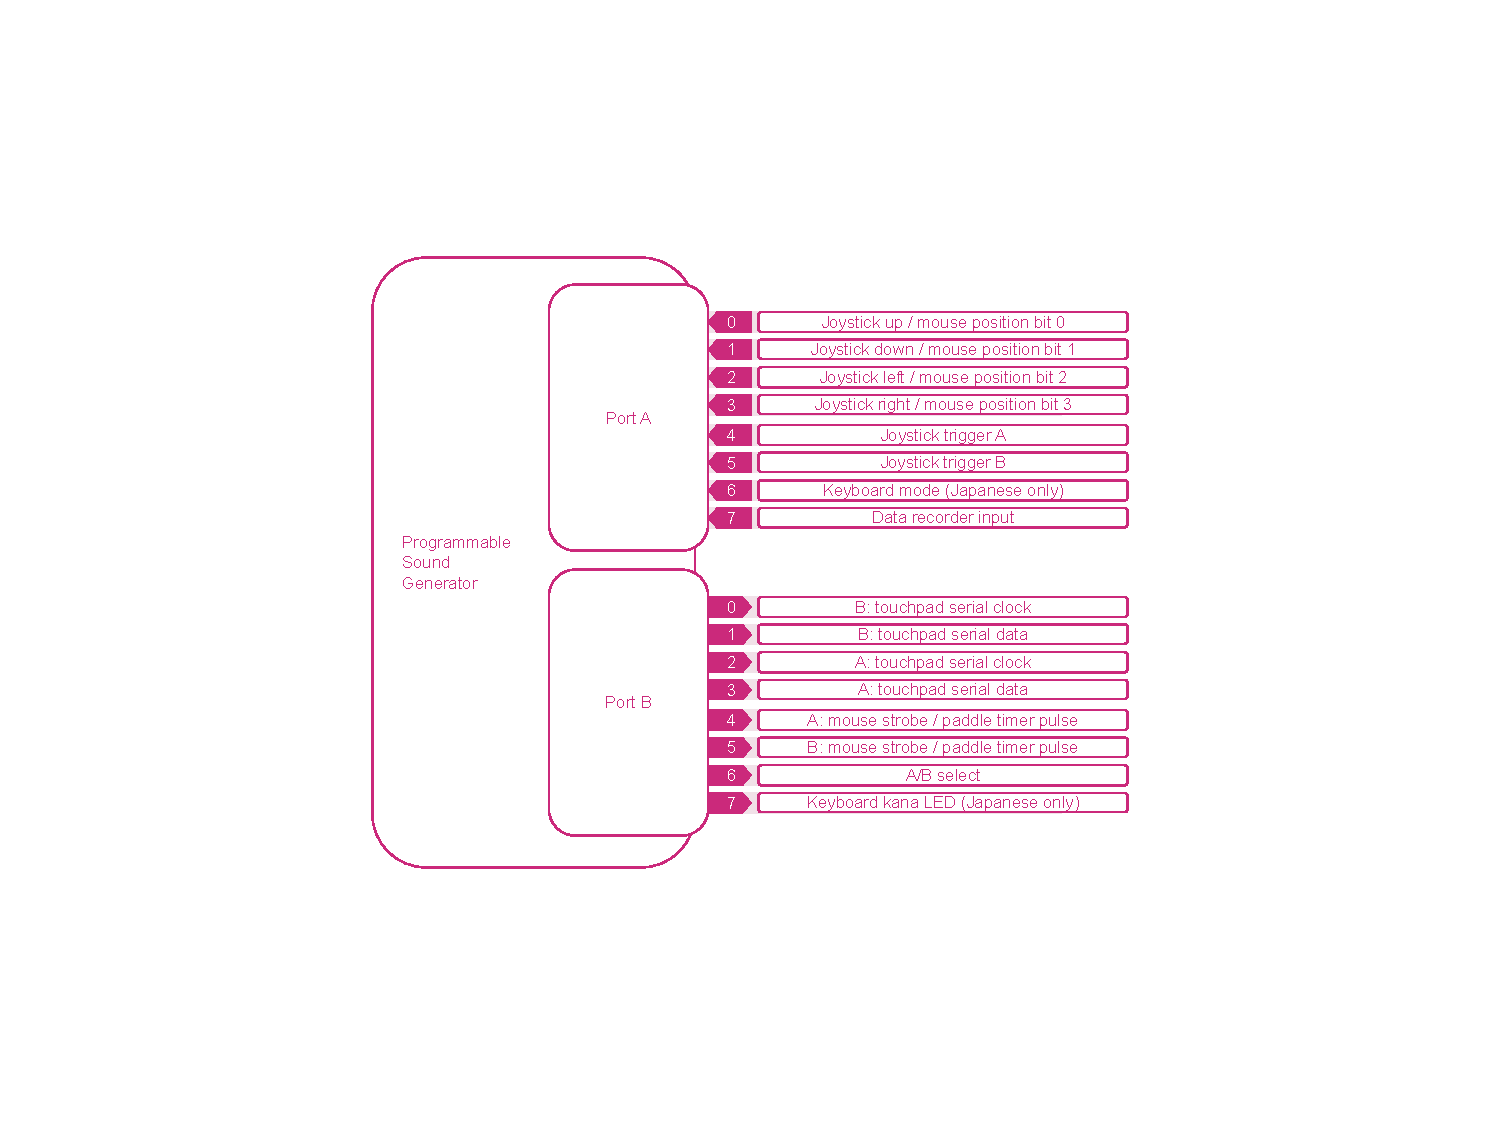
\includegraphics[width=1\linewidth,trim={0cm 120 0 100}]{images/figures/msx-arch-psg-ports}
	\caption{Ports of the MSX Programmable Sound Generator}
	\label{fig:msx-arch-psg-ports}
\end{figure}

The general-purpose ports are informally known as the joystick ports. This is because its main usage is to connect joysticks to the MSX. But they can be also used for many other device types such as mouses, trackpads, paddles, etc. 

The port A of the PSG is configured as input by the MSX BIOS upon system boot. The four less significant bits are used to read joystick movements or mouse position values. The bits 4 and 5 are used to detect whether the trigger A and B is pressed or not, respectively. The bit 6 is used in Japanese MSX models only. It tells what kind of key distribution the computer has, where 1 is JIS and 0 is ANSI. The bit 7 is used to receive the input signal from the data recorder. 

As we have seen before, the data recorder produces a sound signal that is directly connected to the computer. As shown in Figure \ref{fig:msx-arch-psg}, this analog sound signal is converted into a digital equivalent that can be received in the bit 7 of PSG port A. 

The port B of the PSG is configured as output by the MSX BIOS upon system boot. The four less significant bits are used for touchpad devices only to transmit the clock and data signals. For the rest of devices, they will be set to 1. The bit 4 and 5 are the mouse strobe signal or the paddle timer pulses for devices plugged to connector A and B, respectively. The bit 6 is the connector select bit. Did you wonder what device the six less significant bits from port A refer to? Yes, as we can have two joysticks, mouses, etc., it should be possible to read movements from two different devices. The fact is that these six bits from port A are multiplexed. It means the same wires are used to carry the movement information from connector A or B. The bit 6 of port B determines which device will put their information on the wires that connect to PSG port A. Finally, the bit 7 drives the LED of the Kana key in Japanese keyboards.

\subsection{Expansion slots}

We are almost done. There is only one more important part of an MSX system to discuss: the expansion slots. 

As mentioned above, the MSX system was designed with the expansibility in mind. The intention of its authors was to allow the users to add new hardware and increase the capacity of their computers as easily as possible. To achieve this, they designed the computer to have expansion slots. 

You are probably more than used to use expansion slots, also commonly known as cartridge slots. They are 50 pin edge connectors in the motherboard of the MSX where the user can insert cartridges to expand the system. These cartridges are RAM expansions, games, storage devices, floppy drives, sound chips, etc. MSX systems have at least one cartridge slot, but it is not unusual to see models with two slots. In some other cases a cartridge slot is complemented with a 50-pin expansion IDC connector that has the same or similar pinout. The popular Spectravideo SVI-728 is an example of this. 

The expansibility of the cartridge slot is possible because, in essence, the slot connector is an extension of the system bus, as shown in Figure \ref{fig:msx-arch-slots}. Most of the lines that comprise the system bus are included in the 50 pins connector. Thus, connecting a cartridge to the slot is equivalent to having such hardware soldered into the motherboard of the computer.

\begin{figure}
	\centering
	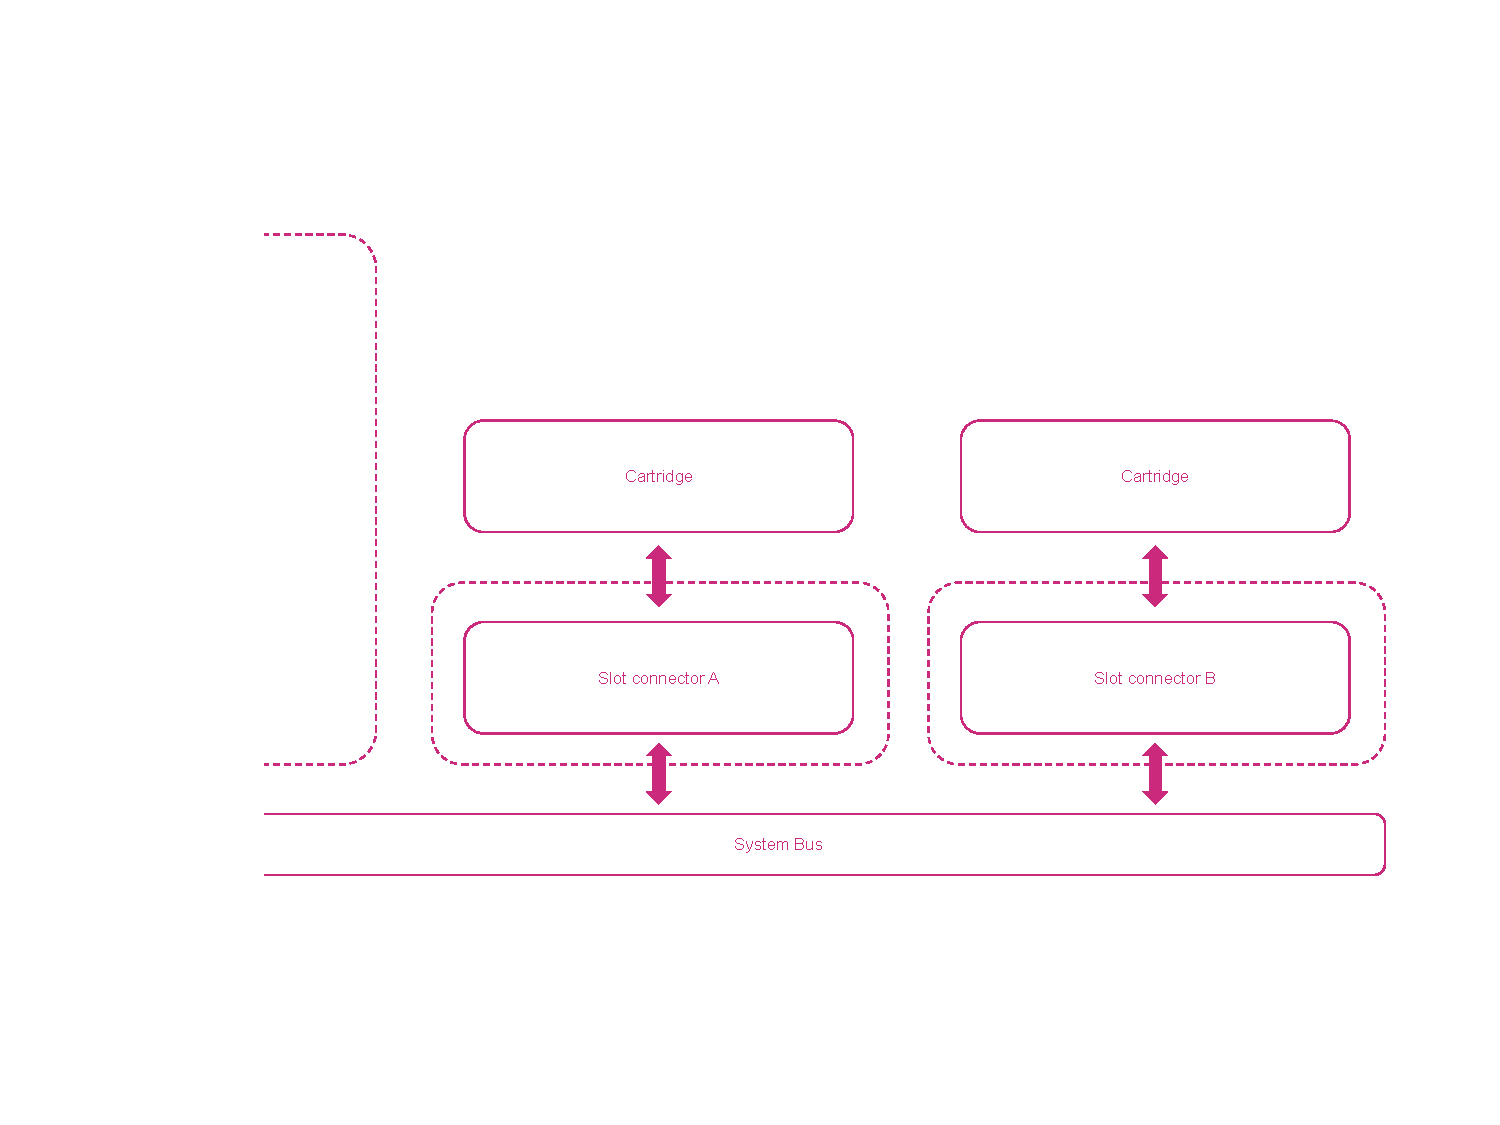
\includegraphics[width=1\linewidth,trim={0cm 120 0 100}]{images/figures/msx-arch-slots}
	\caption{High level architecture of expansion slots in a MSX Computer}
	\label{fig:msx-arch-slots}
\end{figure}

\subsection{Summary}

We have seen an overview of the most important parts that conform an MSX system. There are some others that will not be covered here, such as the serial communications port or the printer port. 

As you can see, and as we revealed at the beginning of this chapter, the architecture of the MSX computer is extremely simple. Compared to other contemporary computers such as the IBM PC, the MSX do not have neither an interrupt nor a DMA controller. It has no mass storage device other than the data recorder and it has no real-time clock. Most of its hardware is based on off-the-shelf components, such as the TMS9918 VDP or the AY-3-8910 PSG. This contrasts with other hardware platforms such as the ZX Spectrum, the Amstrad CPC or even the IBM PC, which mount their own proprietary video display controllers. The MSX was designed to be cost-effective and standard. And this means a simple architecture easy to reproduce. 

As we have seen from the beginning of this chapter, the most complex part of the MSX architecture is the memory system. Due to its relevance, we will dedicate a whole section to it.

\section{MSX Memory Slots}
\label{sec:msx-mem-slots}

\subsection{Bank switching}

The Z80 microprocessor uses 16-bit numbers to represent memory addresses. This means it can reference 65,536 memory locations. Assuming each memory location is 8-bit size, the whole memory space has 64KB. 

In the time when the Z80 CPU was designed, that memory was enough for almost any purpose. But as the computers acquired more power and the user demands increased, the needs for more and more memory also appeared. In 1984, when MSX architecture was set, most computer engineers were incorporating in their designs methods to break the 64KB barrier present in most CPUs. These methods are based on what is known as memory {\bf bank switching}. 

The concept is simple, although the implementation may become cumbersome. Instead of having a single RAM memory region, we will have multiple. Each region will be called a bank. The system determines what memory bank is used by the CPU in each instant in function of some programmable configuration and the memory address that is being used. 

For example, a Z80-based computer can have four banks of 64KB of RAM memory each. If we put them all together, they are 256KB of memory, as shown in Figure \ref{fig:msx-mem-banks}. That is indeed not bad for an 8-bit computer. The software can choose what bank is active using a 2-bit register that is accessible through I/O requests. In this example the two bits could be part of the port of a PPI or similar, as we have seen at the beginning of this chapter. The system BIOS can preconfigure this bank select register with the value 0b00 so the first 64KBs of memory are visible to the CPU. At some point, the program can write the value 0b01 to the bank select register to switch to the memory bank 1. This means the CPU will see after this the memory from 64KB to 128KB. With bank 0b10 and 0b11, the memory segments from 128KB to 196KB, and from 196KB to 256KB, respectively will be visible to the CPU. 

\begin{figure}
	\centering
	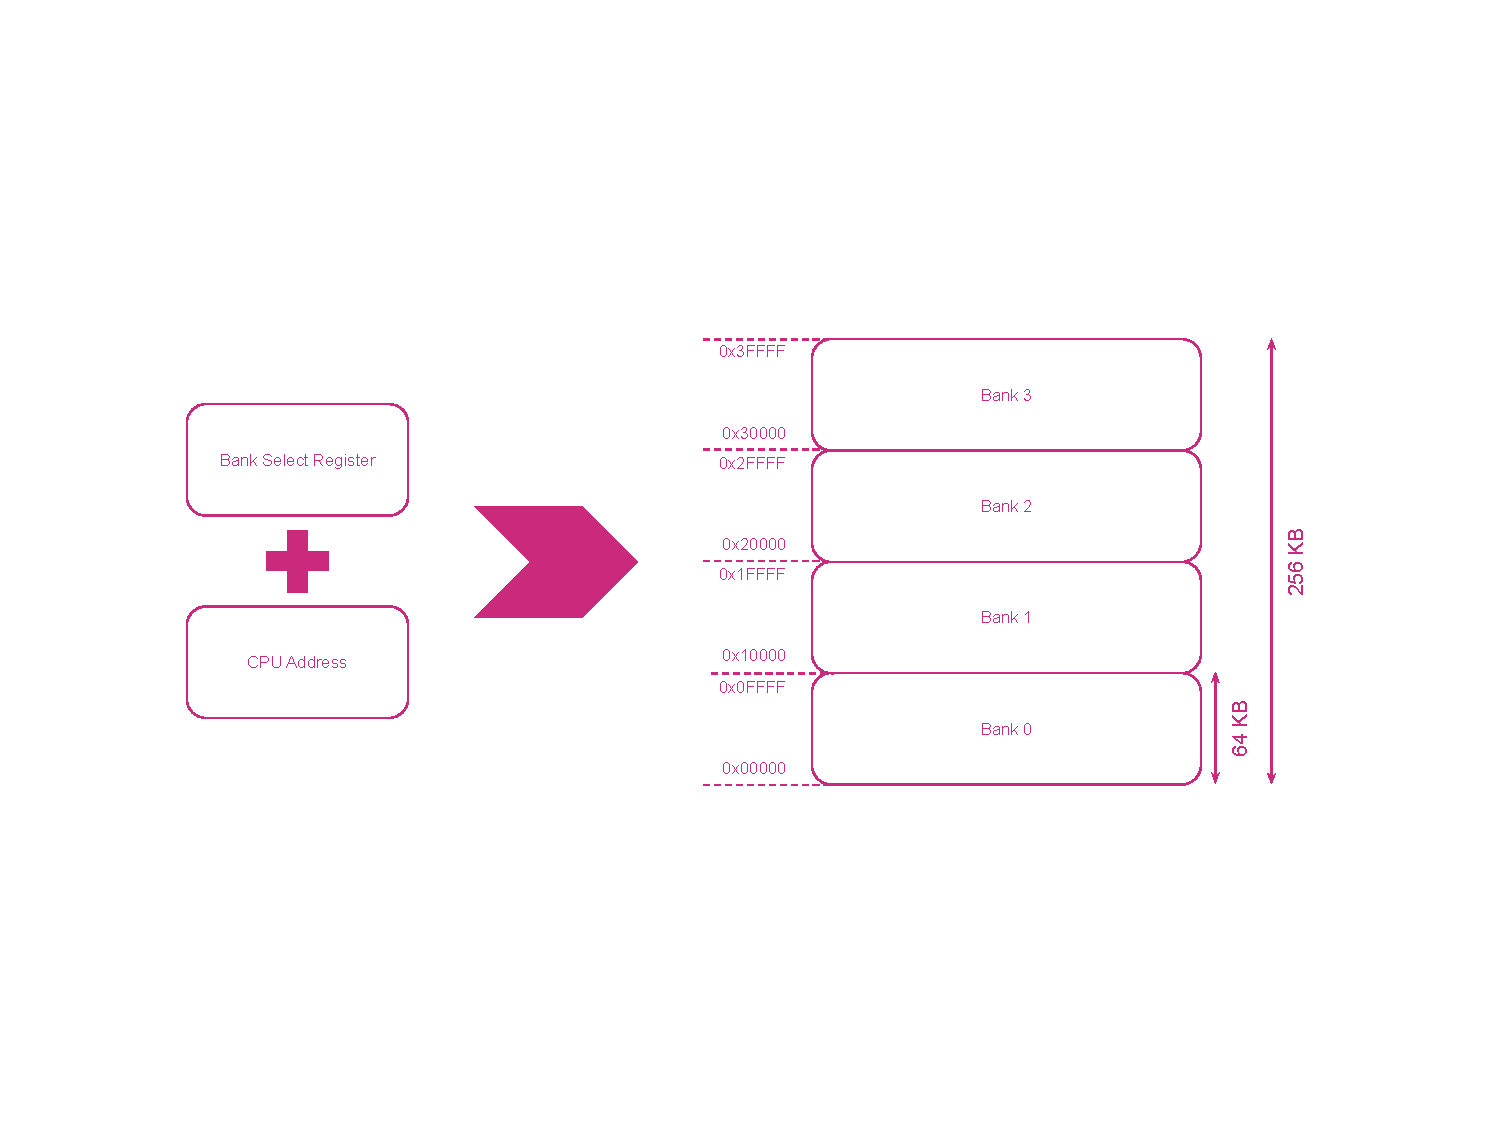
\includegraphics[width=1\linewidth,trim={0cm 150 0 100}]{images/figures/msx-mem-banks}
	\caption{An example of memory bank switching}
	\label{fig:msx-mem-banks}
\end{figure}

If you think about this in terms of memory addresses, you will note we are extending the memory addresses from 16 bits to 18 bits. To distinguish both, we may call the 16-bit address generated by the CPU as logical address and the extended 18-bit address as physical address. The physical address results from concatenating the contents of the bank select register to the logical address. Thus, if bank 2 is selected and the CPU requests an access to the memory location at 0x800A, the physical address will be 0x2800A (0x2 concatenated to 0x800A). 

Unfortunately, this bank switch solution is too naïve and will not work in the real world. This is because we are considering the whole memory space is switched when a new bank is selected. And this interrupts the execution of the program. 

For example, consider a program located at logical address 0x8000 is running with the bank 0 active. This is the physical address 0x08000. At some point, the program decides it needs more memory, so it must switch to the bank 1. After the switch, the memory seen by the CPU at logical address 0x8000 is no longer at physical address 0x08000, but 0x18000. In other words, the program the CPU was executing suddenly disappears. The next instruction the CPU will execute after bank switching is in 0x18000 region of physical memory, which contains uninitialized memory. 

As we already mentioned above, this is typically addressed by also considering the segment of the memory that is being addressed as an input to calculate the memory bank. We can extend our example such as instead of having one bank select register, we have four of them. The first register will indicate the bank of memory space located from logical address 0x0000 to 0x3FFF. The second one is the bank for logical addresses between 0x4000 to 0x7FFF. And the third and fourth bank registers will be used for the logical address space from 0x8000 to 0xBFFF and 0xC000 to 0xFFFF, respectively. 

In the case of a program that is located at physical address 0x08000, the 3rd bank select register will have a value of 0. The rest of register can have any other values, pointing to the same bank or another. If the program decides to make use of more memory, it can switch the 1st, 2nd and 4th bank registers to point to new banks with available memory. But it must not change the 3rd register or the program will suddenly disappear as we have seen before. 

\subsection{MSX Slots}

Although you may find this surprising (or not), what we had described above are the basics of what the MSX system does with its memory.

The MSX divides the 64 KB of the logical address space of the Z80 CPU by four. Each logical address space segment is called a page. The pages are shown in Table \ref{table:msx-mem-pages}.

\begin{table}[h]
	\centering
	\begin{tabular}{r|l|l}
		{\bf Page} & {\bf Start logical address} & {\bf End logical address} \\
		0          & 0x0000                      & 0x3FFF                    \\
		1          & 0x4000                      & 0x7FFF                    \\
		2          & 0x8000                      & 0xBFFF                    \\
		3          & 0xC000                      & 0xFFFF                    \\
	\end{tabular}
	\caption{MSX memory pages}
	\label{table:msx-mem-pages}
\end{table}

The physical memory region that is mapped to each page is called a slot. There are four primary slots, and each of them can be extended by another four secondary slots to a total maximum of 16 slots. But we will cover this later. 

The primary slot configured for each page is determined by the port A of the PPI, as we have seen before. Each pair of bits of that port provide a number from 0 to 3 that tells what slot is used by that page, as we seen in Figure \ref{fig:msx-arch-ppi}. The slots can be reconfigured with I/O write requests to the PPI to switch the bits of the port A. 

That is to configure the slots for each memory page. But what is exactly a slot? In the previous section, we have simplified the example by telling each bank is a 64KB region of RAM memory. But the real life is more complicated. In the real world, we have RAM and ROM memories. And in the case of the MSX, we want to have an extensible system. And that includes adding cartridges with RAM expansion or some hardware that has BIOS extensions written in ROM memories to manage the device. That is why in MSX we talk about slots, and not banks. 

An MSX slot is anything that can respond to memory read and write operations. Typically, an MSX system has some built-in slots with some RAM or ROM memory. While some other slots are provided by… do you guess? Yes! The cartridge slots! 

We had said the cartridge slots are expansions of the system bus. And they are indeed! But each cartridge slot has a designated memory slot. The 50-pin connector incorporates a select signal activated when it is targeted as the active slot when some page is addressed. When this happens, the cartridge connected to the slot must respond to the memory operations when they occur.

An example of this slot organization is shown in Figure \ref{fig:msx-mem-slotsprim}. In this case, the system has two built-in primary slots. The slot 0 contains a ROM memory from address 0x0000 to 0x7FFF. This ROM memory contains the MSX-BIOS and the MSX-BASIC in pages 0 and 1, respectively. Pages 2 and 3 are not wired. The slot 1 is a 64KB RAM memory occupying the for pages. The slots 2 and 3 are connected to the cartridge slots of the computer. In this example, we see a floppy drive connected to the cartridge slot A, which is the memory slot 2. This cartridge contains a ROM memory with an MSX-DISK BIOS extension to manage the floppy drive at memory page 1. In the cartridge slot B, which is the memory slot 3, we had plugged the popular game Arkanoid. This cartridge contains a ROM located at pages 1 and 2 with the game program and data. 

\begin{figure}
	\centering
	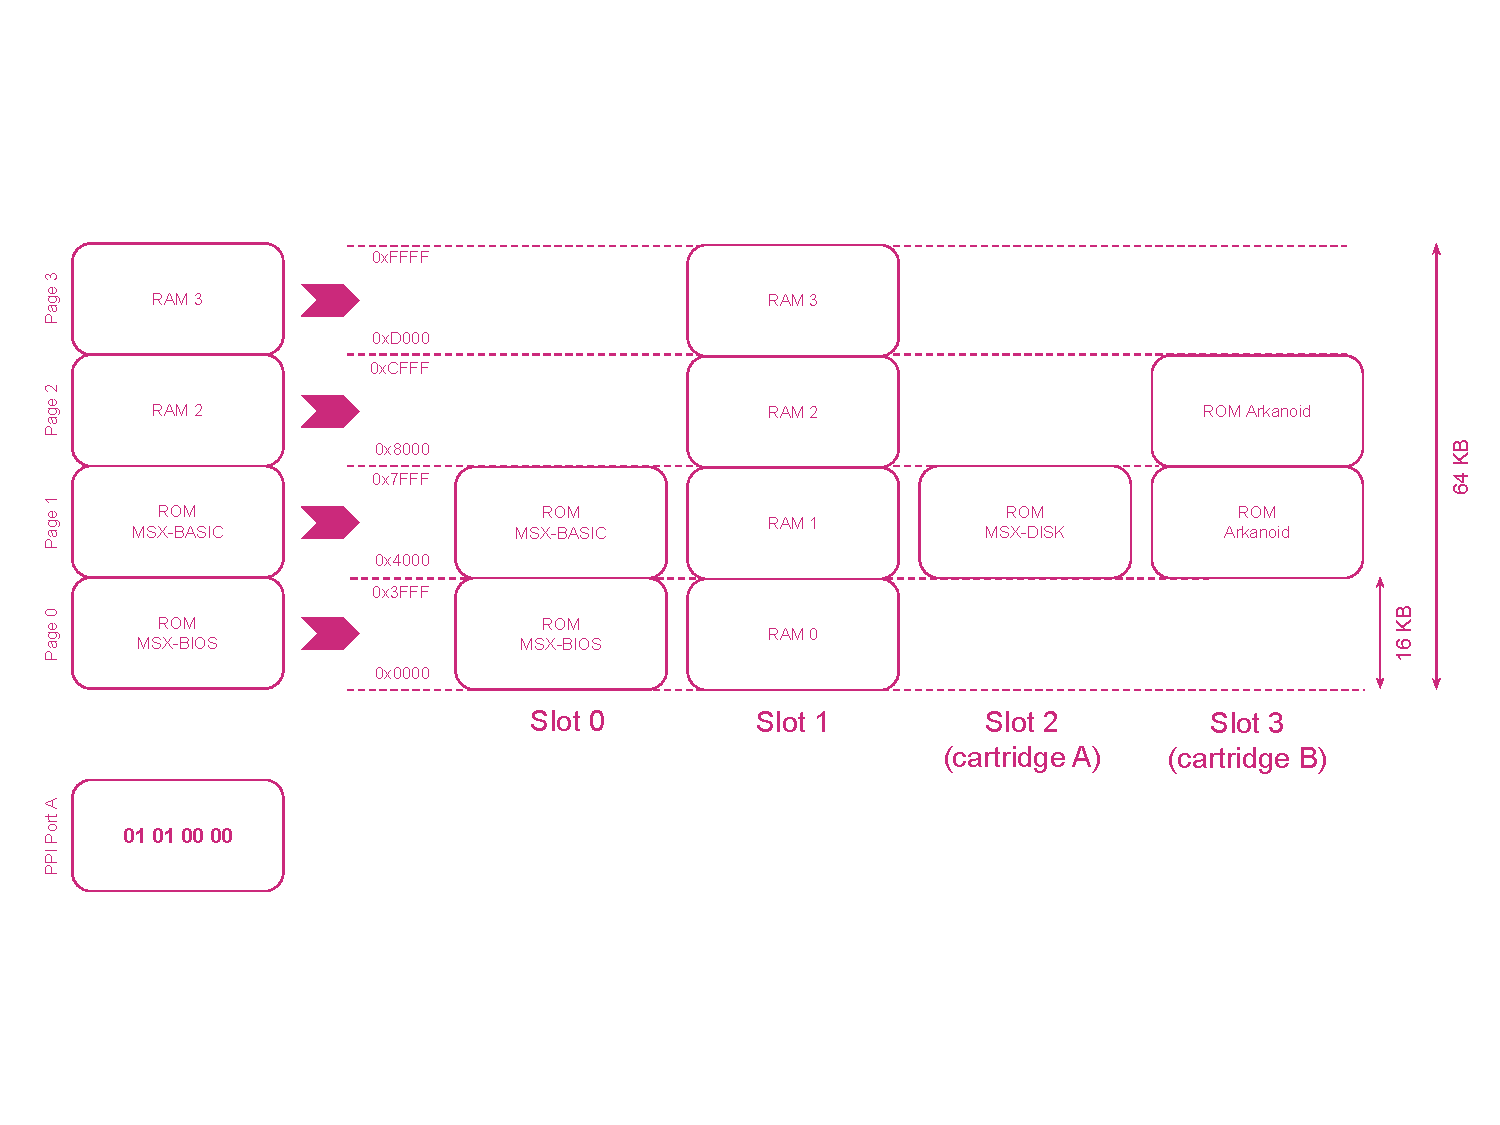
\includegraphics[width=1\linewidth,trim={0cm 100 0 80}]{images/figures/msx-mem-slotsprim}
	\caption{MSX memory slots configuration}
	\label{fig:msx-mem-slotsprim}
\end{figure}

In this example, the PPI port A is set to 0b01010000. This means the page 0 and 1 are mapped to the slot 0. That is why the MSX-BIOS and the MSX-BASIC are visible to the CPU. The page 2 and 3 are mapped to the slot 1. This is the slot full of RAM memory. Thus, the CPU will see RAM memory in the two upper pages. 

Now let us say we load a program from the data recorder to the RAM at page 2 and run it. The code of the program can determine it needs more RAM than the 32KB already mapped. In order to use more RAM, it can configure the RAM slot in the page 1 by writing 0b01010100 to the PPI port A. Thus, it gets rid of the MSX-BASIC code to increase the RAM to 48KB. If the program needs even more RAM, it can configure the slot 1 for page 0 as well, such that the whole address space is full of RAM. 

Please note the slot reconfiguration is not irreversible. Even in the case the program needs the whole 64KB of RAM memory, it does not mean it cannot use the MSX-BIOS anymore. For example, it might configure page 0 to use the RAM slot only when it must read or write to it. And once finished, restore the slot configuration to have again the MSX-BIOS code in the page 0. The same principle applies to any other memory page. There is only one restriction in this model: you cannot change the slot of the page where the current program is running. Because as we have seen before, this will interrupt the program. 

One important note: the slot distribution seen here is just an example. The MSX standard does not indicate any specific memory layout. Some vendors decide to use the slot 1 for RAM. Some others use the slot 3. And they put the cartridges in slots 1 and 2. Some others only have 1 cartridge slot, so one of the memory slots is not used. Each vendor decides their own slot distribution. The software or the users must not make assumptions on where each memory device is located. Such assumptions had caused historical incompatibilities by some software that do not run properly on some MSX computers.

\subsection{Secondary memory slots}

Finally, it is time to discuss about the expanded slots. We already mentioned that each slot can be expanded such that it can contain four secondary slots. It means this slot will respond to read and write operations by forwarding the request to another sub-slot. The MSX standard specifies a way to configure the sub-slot that will attend the memory accesses when the primary slot is selected in the PPI. This is with a register located in the address 0xFFFF of the primary slot. This register operates in the same way as the port A of the PPI, with each pair of 2 bits selecting the sub-slot that will be used for each memory page. 

Let us see this with an example, shown in Figure \ref{fig:msx-mem-slotssec}. Some MSX system may have the slot 1 expanded with two sub-slots. The sub-slot 0 contains 4 pages of RAM. The sub-slot 1 contains one page of ROM with some MSX-BIOS expansion. This primary slot 1 has a hardware register that responds to read and write operations at the address 0xFFFF. 

\begin{figure}
	\centering
	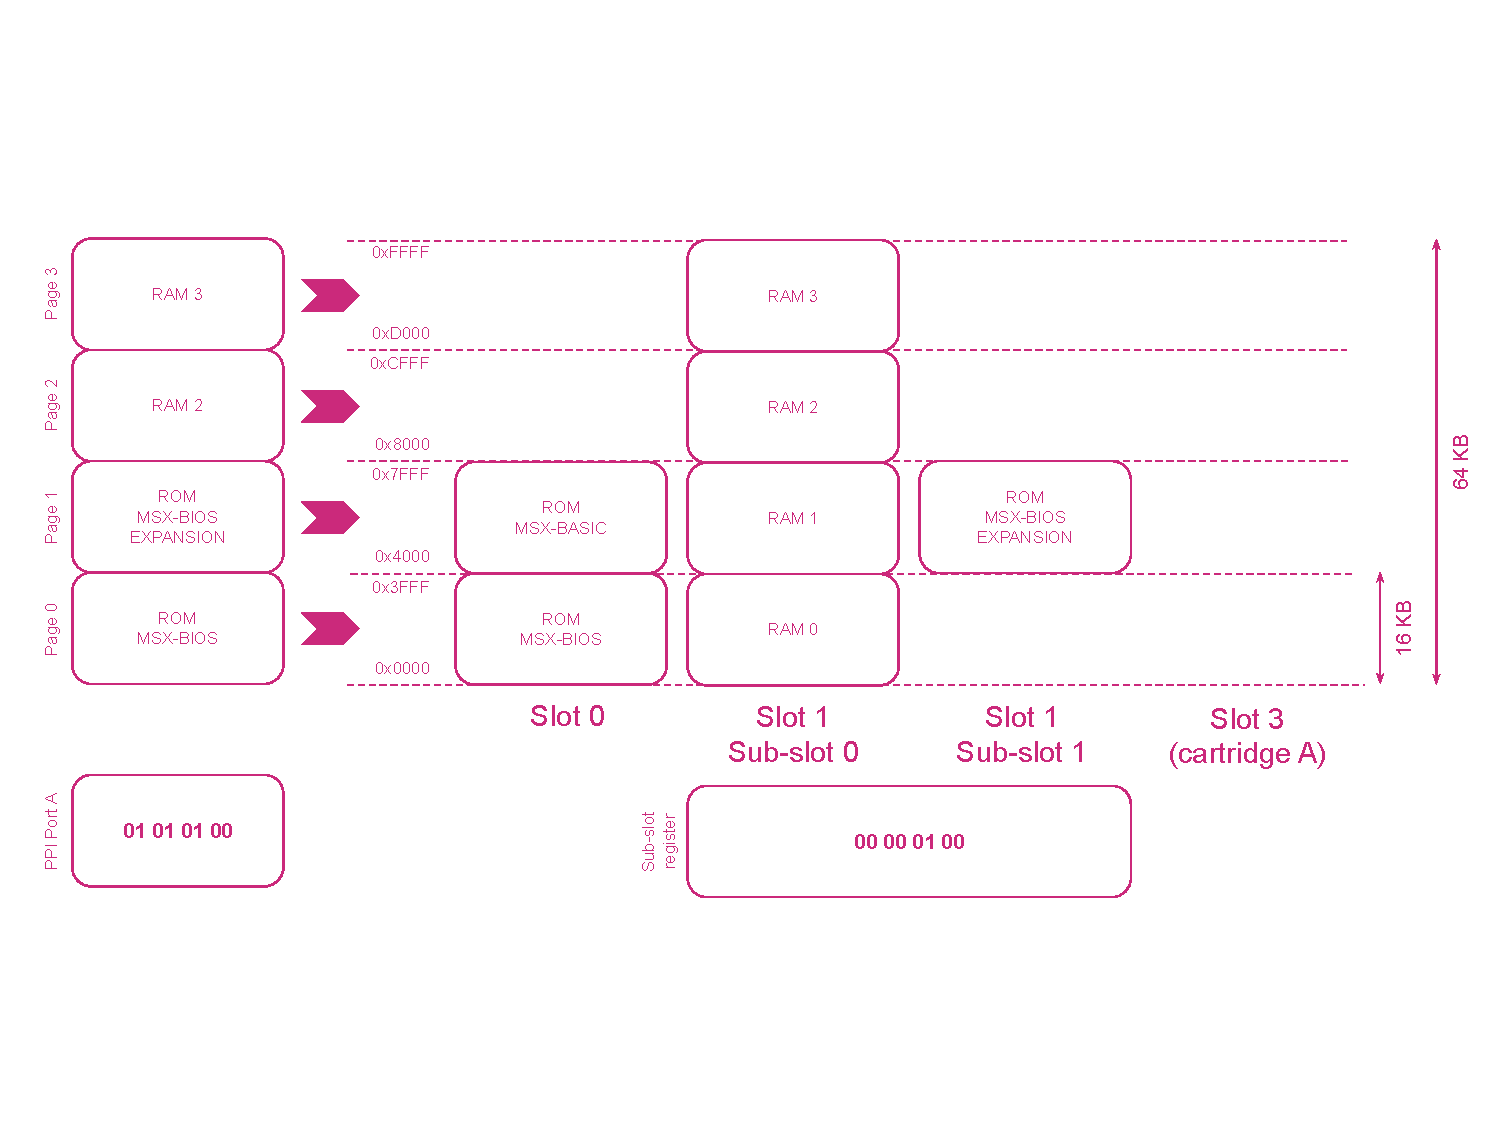
\includegraphics[width=1\linewidth,trim={0cm 100 0 80}]{images/figures/msx-mem-slotssec}
	\caption{MSX secondary memory slots configuration}
	\label{fig:msx-mem-slotssec}
\end{figure}

If we want to map the page 2 and 3 to RAM, we must:
\begin{itemize}
	\item Configure the pages 2 and 3 to use the primary slot 1. This means writing the value 0b0101xxxx to the PPI port A.
	\item Configure the register of primary slot 1 to use sub-slot 0 for pages 2 and 3. This means writing the value 0b0000xxxx to the register of slot 1 at address 0xFFFF.
\end{itemize}

Analogously, to have the MSX-BIOS Expansion accessible at page 1, we must:

\begin{itemize}
	\item Configure the page 1 to use the primary slot 1. This means writing the value 0bxxxx01xx to the PPI port A.
	\item Configure the register of primary slot 1 to use sub-slot 1 for page 1. This means writing the value 0bxxxx01xx to the register of slot 1 at address 0xFFFF.
\end{itemize}

As you might figure out, accessing the address 0xFFFF in certain primary slots is tricky. A primary slot will respond to that address only when page 3 is configured to use that slot because address 0xFFFF belongs to page 3. Thus, in certain configurations it is necessary to configure the page 3 to use that slot first, and then write to the address 0xFFFF to set the sub-slot configuration. After this, we must restore the previous configuration of the primary slots to leave the things in a consistent state. 

But the problems do not end there. As we mentioned above, the MSX standard does not impose any specific slot layout. The users and their software must not make any assumption about where RAM or ROM is located. This implies the software, including the MSX BIOS, must be able to discover where the memory is. This can be done with a subprogram that scans the slots looking for RAM memory. But how can it determine if a primary slot is expanded or not? Consider an expanded slot has a register at address 0xFFFF. But a primary slot may have a RAM memory in this very address. In both cases, this address can be written and read. How could the software say if this is a cell in a RAM memory chip or it is a hardware register?

The MSX standard has an answer to this. It states that the hardware register of an expanded slot must respond by inverting the contents when the register is read by the CPU. Thus, if the software writes 0b01010101 to the address 0xFFFF of a primary slot and immediately after that it reads back what was written, there are three possible results:

\begin{itemize}
	\item 0b01010101. The same value that was written. It means this slot contains RAM and it is not expanded.
	\item 0b10101010. The value that was written with its bits inverted. It means this slot is expanded.
	\item Any other value. The slot does not have anything responding to write operations at 0xFFFF. It means indeed the slot is not expanded. It might be a primary slot with ROM at page 3, the slot is not connected, or it is a cartridge slot that has nothing plugged.
\end{itemize}

As you can see, the memory slots system is rather complex but powerful. Each memory page can be mapped to a maximum of 16 different slots. This is a total address space of 1 megabyte of memory. Not bad considering that 640 KB ought to be enough for everybody. 


\chapter{Artemisa System Architecture}

Once we have a high level architectural view of how an MSX computer works, it is time to start the discussion around how an Artemisa computer implements that architecture.

\section{Features of Artemisa Model 101}

The Artemisa Homebrew DIY model 101 implements most of the parts of the MSX standard have we seen above.

In a few words, Artemisa is an MSX computer with 64KB of RAM memory and two cartridge slots. It has two general purpose (joystick) ports, a data recorder connector, an external keyboard and an interchangeable graphics card. All this encapsulated in a transparent acrylic case of 300x150x35 millimeters.

There are just a few things you typically find in an MSX computer that are not present in Artemisa:

\begin{itemize}
  \item Serial communications port. This can be used to connect modems or other communication devices.
  \item Printer port. Used for printing.
  \item +12- and -12-volts power lines. The built-in hardware of Artemisa use 5 volts power only.
\end{itemize}

However, the +12- and -12-volt lines are included in the pinout of the cartridge connectors. Artemisa wires these pins to ground instead.

\subsection{Keyboard}

Most of the MSX computers, as many other microcomputers built during the 80s, had an integrated keyboard. These computers look like a big keyboard that contains all the elements inside. In contrast, a few MSX vendors followed the same approach as IBM did with their PC: separate the keyboard from the computer connected through a keyboard port. This makes the system less integrated. But also brings some benefits. First, the keyboard can be easily replaced in case of failure. Second, it is easier to manufact computers at scale with different keyboard distributions and layouts, as they only differ in the keyboard.

Artemisa also uses an external keyboard to get advantage from these benefits: reduce the design cost and let the user to choose their keyboard option. It has a custom 25-pin connector that can be used to connect an external keyboard. This can be a custom keyboard built for the Artemisa, or an adapter that allows to connect a PS2 or a USB keyboard.

The Artemisa Homebrew DIY model 101 is shipped by default with a PS2 adapter. You can use it to connect a regular, unexpensive PC keyboard. A microcontroller into the adapter will map the scancodes from the PS2 protocol to simulate a keyboard matrix the MSX will see connected to the port.

\subsection{Graphics card}

The same reasons to have a separated keyboard also applies to have a separated graphics device. Each region has its own TV encoding standards. Some countries use NTSC. Some others use PAL. Some users prefer an unexpensive device that uses composite video output. Some others prefer a RGB output via an SCART connector.

In order to simplify the design and allow the users to customize the video output according to their needs, Artemisa Homebrew DIY separates the graphics card from the rest of the computer motherboard. Both are internally connected using a 50-pin ribbon cable.

\subsection{CMOS Technology}

We will not go too deep in this subject, but it might be worth to discuss a little bit about the semiconductor technologies behind Artemisa.

As you probably know, there was a key invention that boosted the development of computer systems: the transistor. This semiconductor device is the most basic building block used to make basic digital circuits such as logic gates. There are multiple technologies used to implement transistors depending on the semiconductor materials used in the process. Each technology has different properties, constraints and tradeoffs.

During the 70s and 80s, the most used transistor type in consumer electronics was the bipolar junction transistor (BJT). The BJT transistors were the foundations of the Transistor-Transistor Logic technology, or TTL. One of its subfamilies, the TTL-LS, was the de-facto standard used in early microcomputers. The TTL-LS devices switch relatively quick from one logic state to another. This means they have low propagation delays (a voltage change in the input of a gate is quickly reflected in the output voltage), and they can operate at high frequencies (many voltage changes per second can occur). However, this comes in exchange of a high power-consumption. Also, the current they can drive is quite limited. This affects the number of input devices than can be connected to the same output of a TTL device, what is known as the fan-out problem.

In the middle of the 80s, another technology displaced TTL-LS in the consumer electronics market. It was the Complementary Metal-Oxide-Semiconductor (CMOS) technology. It was made up by Metal-Oxide-Semiconductor Field-Effect Transistors (MOSFET). CMOS had two interesting characteristics compared to TTL devices. First, they had a low static power consumption. This means CMOS devices consume much less power than TTL devices when the voltage of their inputs is not changing. Fortunately, for nearly all logic gates in a computer, this is most of the time. This had an interesting side effect: the integration scale is significantly increased. Less power consumption means more transistor density in a chip core (without making the chip burn), what leads to miniaturization. In fact, modern inventions such as the microprocessor were possible thanks to the MOSFET transistors and the derived logic families like NMOS and CMOS. Secondly, CMOS devices can drive more load than TTL equivalents. This practically eliminates the fan-out problem from the equation. These devices also have a better electrical noise reduction. However, the toll paid by CMOS devices is their speed. They respond relatively slow to the changes in their logic state. What cause relatively large propagation delays compared to TTL devices and force them operate at low frequencies. Fortunately, a subfamily known as High-speed CMOS (HCMOS) reduced the propagation delays to acceptable levels.

Roughly speaking, you can assume a TTL logic gate consumes 1000 times the power of its CMOS equivalent. In the other hand, a CMOS device has propagation delays 2x to 5x bigger than their TTL counterparts. The good news is that an MSX computer is a relatively slow machine. The CPU operates at 3.58Mhz and each interaction with the system bus typically involves several clock cycles. The response times are in the range of hundreds of nanoseconds. That is by far in the range of the capabilities of the HCMOS devices.

Taking these considerations, Artemisa uses CMOS devices where possible instead of the TTL equivalents used in the MSX computers designed during the 80s. The glue logic is implemented by integrated circuits of the 74HC family. And the system is designed to operate with Z84C00 and 82C55 chips, the CMOS versions of Z80 microprocessor and the PPI, respectively. There are just a few TTL chips in the design that do not have CMOS equivalents, such as the 74LS07.

\subsection{Integration level}

As discussed in the beginning of this book, Artemisa Homebrew DIY wants to make you learn how an MSX works while you assemble and solder its parts. The easier the assembling process the better. That is why this version of Artemisa sacrifices the miniaturization in favor or an easier soldering experience.

As consequence, all the chips used in the design have Dual Inline Package (DIP) encapsulation.  These are the classic chips used in early microcomputers, formed by two lines of broad pins with a separation of 2.55mm. The same principle is applied to the rest of components. Resistors and capacitors have Through Hole (TH) encapsulation to facilitate the manipulation.

\subsection{Memory technology}

The RAM memory was one of the main limitations of early microcomputers. And not for performance reasons, but costs. Memories were really expensive these days. And engineers had to find ways to make them as affordable as possible.

All RAM memories are made by several x-y matrices of bit cells. For read and write operations, the chip expects to receive the row and column addresses in order to activate the cell where that bit is located and perform the operation. Typically, the bits of the physical memory address are split in two halves such that n less significant bits are the row address and m most significant bits are the column address in the memory matrices. By having eight matrices, one per each bit in a byte, we can implement the system memory of an 8-bit computer.

There are two principal technologies to build RAM devices: DRAM and SRAM. DRAM technology is based on a combination of one capacitor and one transistor to implement each bit cell. The capacitor is used to determine whether the cell contains a logic 1 (charged) or a logic 0 (discharged). The transistor is used as a switch to control the access to the capacitor. Each bit cell is put in a x-y matrix that is addressed by row and column. As it uses only two elements that can be built into a microchip, DRAM is unexpensive compared to other memory technologies.

Unfortunately, DRAM have a big drawback: capacitors tend to discharge by their own. With the time the charge leaks away, so a charged capacitor representing a logic 1 passes to represent a logic 0. Considering the small size of these capacitors, this discharge time is in the order of milliseconds. The RAM chips must refresh the contents of its cells periodically to prevent information lost. In most of the cases, they cannot do that by themselves. And require external circuits to perform the refresh actions periodically. In addition, DRAM chips typically multiplex the pins used for row and column addresses. They depend on a multiplexor circuit to decode the bits from the address bus that belong to row and column. Both the refresh and the row/column multiplexor circuits are not trivial, and they complicate the design of the system.

The alternative to DRAM is the Static RAM (SRAM). This kind of memory uses pure semiconductor devices to implement bistables that can keep 1 bit of information. Typically, six MOSFET transistors are needed per bit cell. What makes them much more expensive than the DRAM equivalents. However, as they do not use capacitors there is no need for refresh circuits.
In the present, the DRAM is still used in modern computers with gigabytes of memory due to its density. SDRAM and DDR technologies are DRAM. However, vendors do not produce DRAM chips for small memory amounts any longer. The SRAM technology has evolved enough to become an unexpensive solution in the range of kilobytes and megabytes. All parts traditionally used in 80s computers are obsolete. And replaces are only available in the secondhand market.

Because of this, and the fact that it simplifies the design of the system, Artemisa uses SRAM memory instead of DRAM. Thanks to this, it does not have to implement a memory refresh circuit or a row/column address multiplexing.

\subsection{Memory layout}

As discussed above, the MSX standard does not define how much memory an MSX computer must have or how it is distributed along the different memory slots.

Artemisa has 64KB of RAM memory located in memory slot 1. These are 4 pages of RAM that occupy the whole slot.

Concerning ROM memory, Artemisa has 32KB of ROM memory where MSX System (MSX BIOS plus MSX Basic) can be found as almost any other MSX system. However, the motherboard provides up to 512KB of total ROM memory. As only 32KB of it are mapped to the MSX in the pages 0 and 1 of memory slot 0, this means the ROM memory has up to 16 different regions of 32KB. Each region contains a different image of the MSX System. A set of 4 jumpers in the motherboard can be used to select the image that will be mapped in the MSX memory space.

The reason to have multiple interchangeable MSX System images is to choose different versions of it, each one supporting different regional configuration. The MSX System image for USA is not the same as the MSX System image for Spain. They expect different keyboard distributions, use a different character set and, in some cases, they even have a different bootscreen message.

\begin{table}[h]
  \centering
  \begin{tabular}{r|l}
    {\bf Jumper config} & {\bf ROM contents}            \\
    {\tt 0b0000}        & MSX System v1.0 International \\
    {\tt 0b0001}        & MSX System v1.0 USA           \\
    {\tt 0b0010}        & MSX System v1.0 Japan         \\
    {\tt 0b0011}        & MSX System v1.0 UK            \\
    {\tt 0b0100}        & MSX System v1.0 France        \\
    {\tt 0b0101}        & MSX System v1.0 Germany       \\
    {\tt 0b0110}        & MSX System v1.0 Italy         \\
    {\tt 0b0111}        & MSX System v1.0 Spain         \\
    {\tt 0b1000}        & MSX System v1.0 Arabic        \\
    {\tt 0b1001}        & MSX System v1.0 Korea         \\
    {\tt 0b1010}        & MSX System v1.0 Russia        \\
    {\tt 0b1011}        & Artemisa Diagnosis Tool v0.1  \\
  \end{tabular}
  \caption{MSX System images stored in the ROM memory}
  \label{table:artemisa-rom-imgs}
\end{table}

The Table \ref{table:artemisa-rom-imgs} summarizes the contents of the Artemisa ROM distribution and the jumper configuration to activate each. As you can see, most of them are MSX System versions. The last one, activated with the jumper configuration 0b1011, is the Artemisa Diagnosis Tool. This is a utility that replaces MSX Basic in order to perform some basic system checks that could be of help diagnosing system problems.

\section{High level architecture}

Now it is time to have a look to the high level architecture of an Artemisa computer. And, what could be better than showing an schematic diagram of the topmost components that comprise the design? This is what you will get from Figure \ref{fig:artemisa-arch-overview}. As you can see, it is likely you are already familiarized to the components shown in that schematic diagram. They are mostly the same elements we have discussed in the previous chapter.

\begin{figure}
  \centering
  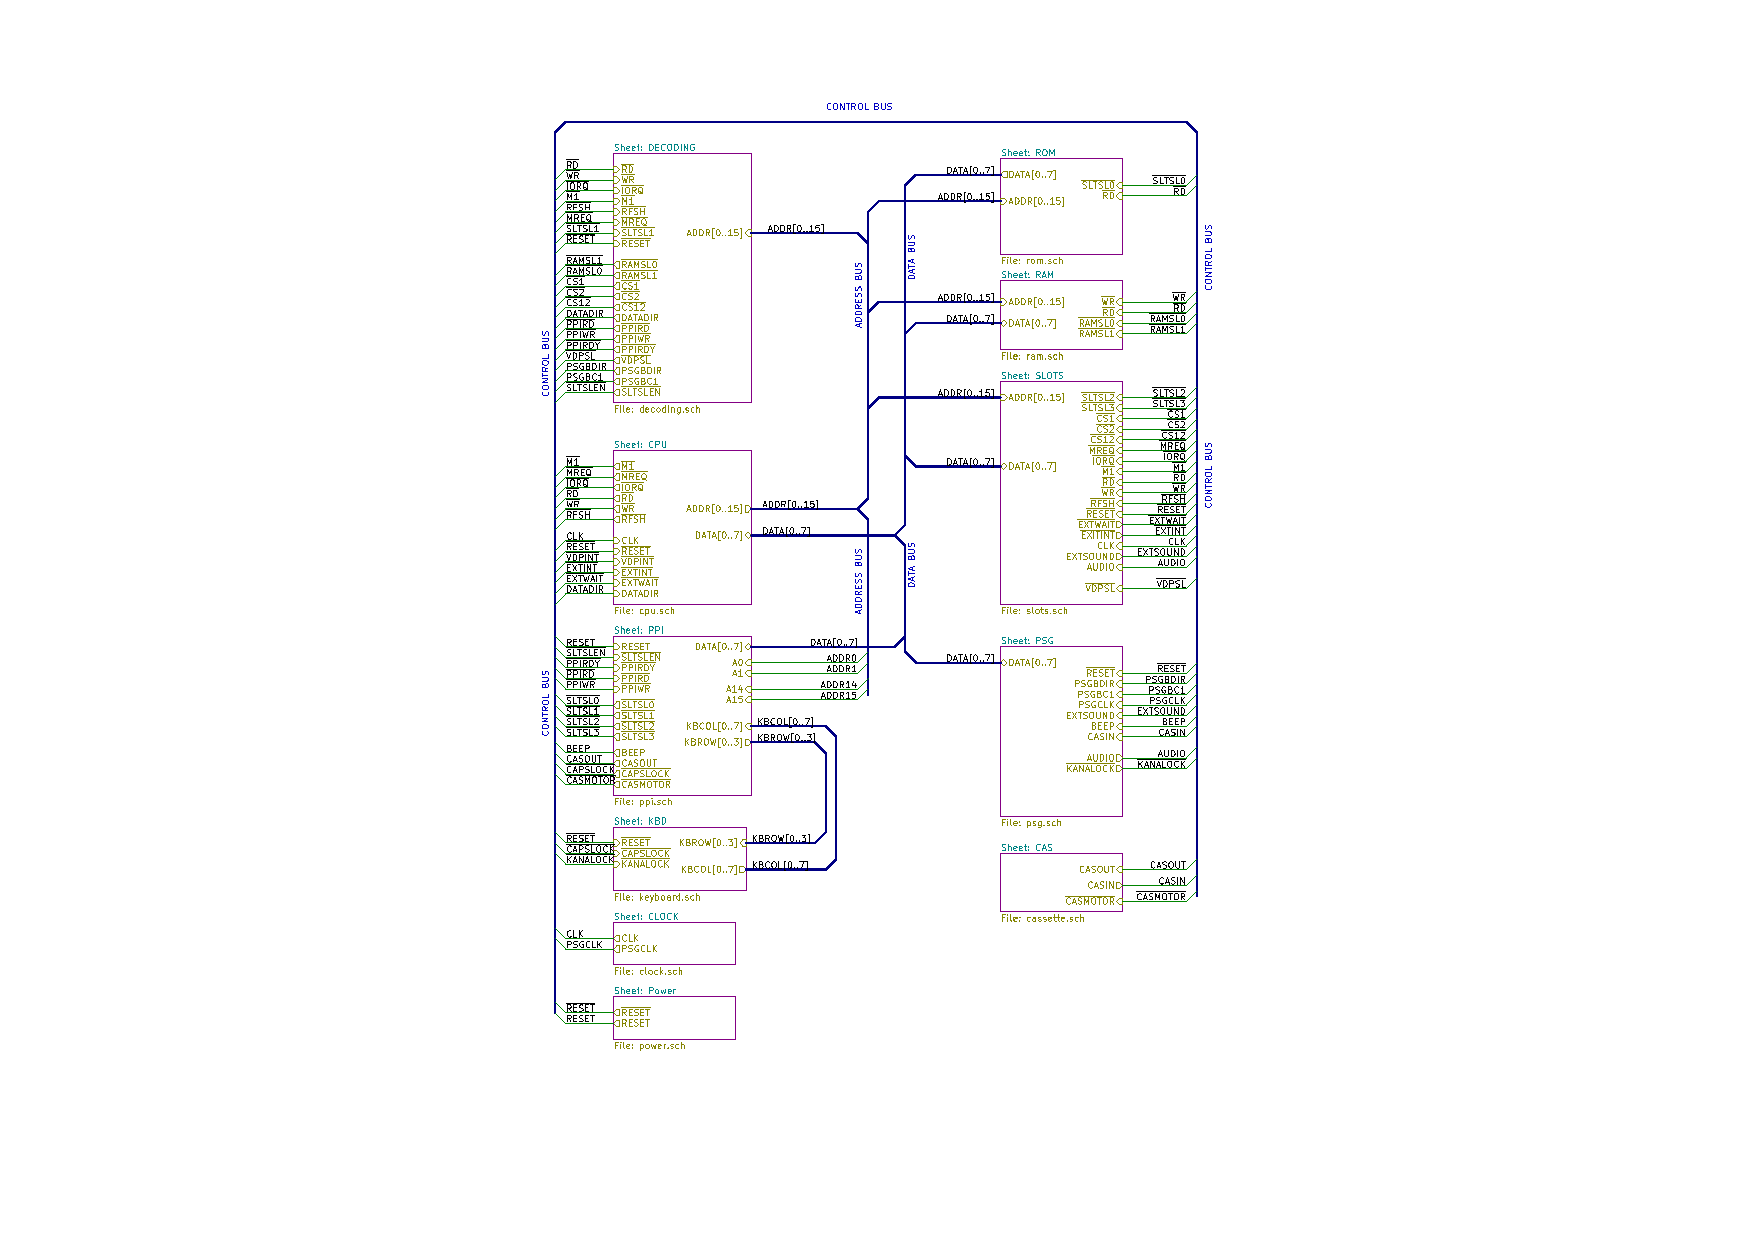
\includegraphics[width=\linewidth,trim={9cm 3cm 9cm 3cm}]{figures/artemisa-schematic-all}
  \caption{High level schematic diagram of an Artemisa MSX Computer}
  \label{fig:artemisa-arch-overview}
\end{figure}

The schematic diagram shows 11 schematic sheets. Each sheet represents a section of the circuit that can be studied separately. You can see the sheets as they were independent integrated circuits or components. In fact, they have pins as any other chip. And the pins are connected to other pins through wires and buses, as in any other schematic diagram. This is what each schematic sheet represents:

\begin{itemize}
  \item {\tt POWER} is the power management sheet. The power connector and the related elements needed to energize the motherboard are described here. The \toref{Power-On Reset} circuit, which is closely related to the power management, is also included here. This is why the outputs of this sheet are mainly the {\tt RESET} and {\tt /RESET} signals.
\end{itemize}

\begin{theory}{Power-On Reset}
  Although this might sound trivial and irrelevant, power-on and reset have a great importance. Once the user presses the power switch on, every component of the system will be energized. They will receive voltage and current from the power supply. But what happens after that?\\\\

  Some elements of the system are implemented with something known as {\it sequential logic}. This means they generate their outputs depending not only in their current input signals but also in a sequence of other inputs occurred in the past. They are designed as state machines that will have a different behavior depending on the state they are at each moment. That is the case of the CPU, the VDP, the PSG, the PPI... If we just power on the system, what will be their initial state?\\\\

  We can find a good example of sequential logic in the CPU. As you might know, the processor contains an internal register known as the Program Counter (PC). This register indicates the memory address of the next instruction to be fetched. But, what is the value of that register when the CPU is powered on? What will be the first instruction to be executed then?\\\\

  The CPU, and any other integrated circuit implemented with sequential logic, provides an input pin where it can receive a signal to be reset into their initial state. This is not only useful when we want to reboot the computer by pressing a reset button, but also when the system is powered up. Receiving electrical current does not mean the state machine will be reset. We have to generate a reset signal when the system is powered up. And... we will see later that this is not as simple as it sounds!
\end{theory}


\begin{itemize}
  \item {\tt CLOCK} is the clock generation circuit. This is a small schematic sheet that will produce squared wave signals of 3.58Mhz and 1.78Mhz used by the Z80 CPU and the AY-3-8910 PSG, respectively.
  \item {\tt CPU} is the sheet where Z80 CPU circuitry is described. This includes all the glue logic to buffer the buses used by the CPU, and the circuit to handle the wait states required by the CPU. If you already know the Z80 CPU pinout, the inputs and outputs of this sheet should be familar.
  \item {\tt DECODING} is the bus decoding logic. This is where the signals from control and address buses are decoded to generate other signals to select actions for other components attached to the buses.
  \item {\tt ROM} is the sheet where the ROM memory is designed.
  \item {\tt RAM} is the sheet where the RAM memory is designed.
  \item {\tt PPI} is the sheet where the Parallel Peripheral Interface is designed. This includes some glue logic necessary to adapt some interfaces.
  \item {\tt PSG} is the sheet where the Programmable Sound Generator is designed. This includes some circuits to adapt the game port interfaces.
  \item {\tt SLOTS} is the sheet where the expansion slots are designed. This includes the connector for the graphics card.
  \item {\tt CAS} is the sheet where the cassette data recorder is designed. This includes the circuits to encode and decode the cassette analog to digital signals.
  \item {\tt KBD} is the sheet where the keyboard interface is designed.
\end{itemize}

Apart from the schematic sheets, we can see in Figure \ref{fig:artemisa-arch-overview} they are also connected among them through a set of buses. These are the control, the address and the data buses we discussed in the previous chapter. But there are also two additional ones: {\tt KBCOL} and {\tt KBROW}. They are the columns and the row address from the keyboard matrix we have also seen before.

As we said in the previous chapter, the design of a 8-bit microcomputer is quite simple. The Figure \ref{fig:artemisa-arch-overview} is all we can find in the motherboard of the Artemisa 101 series. Of course, each schematic sheet contains many elements, so the level of complexity increases as we go deeper in the design. But you do not have to worry. Thanks to having all the elements separated in submodules, we will have the opportunity to cover them separately without feeling overwhelmed.

\section{Anatomy of the Artemisa Model 101}

When all the things are put together into a printed circuit board, the result is as shown in Figure \ref{fig:artemisa-anatomy}.

\begin{figure}[h]
  \centering
  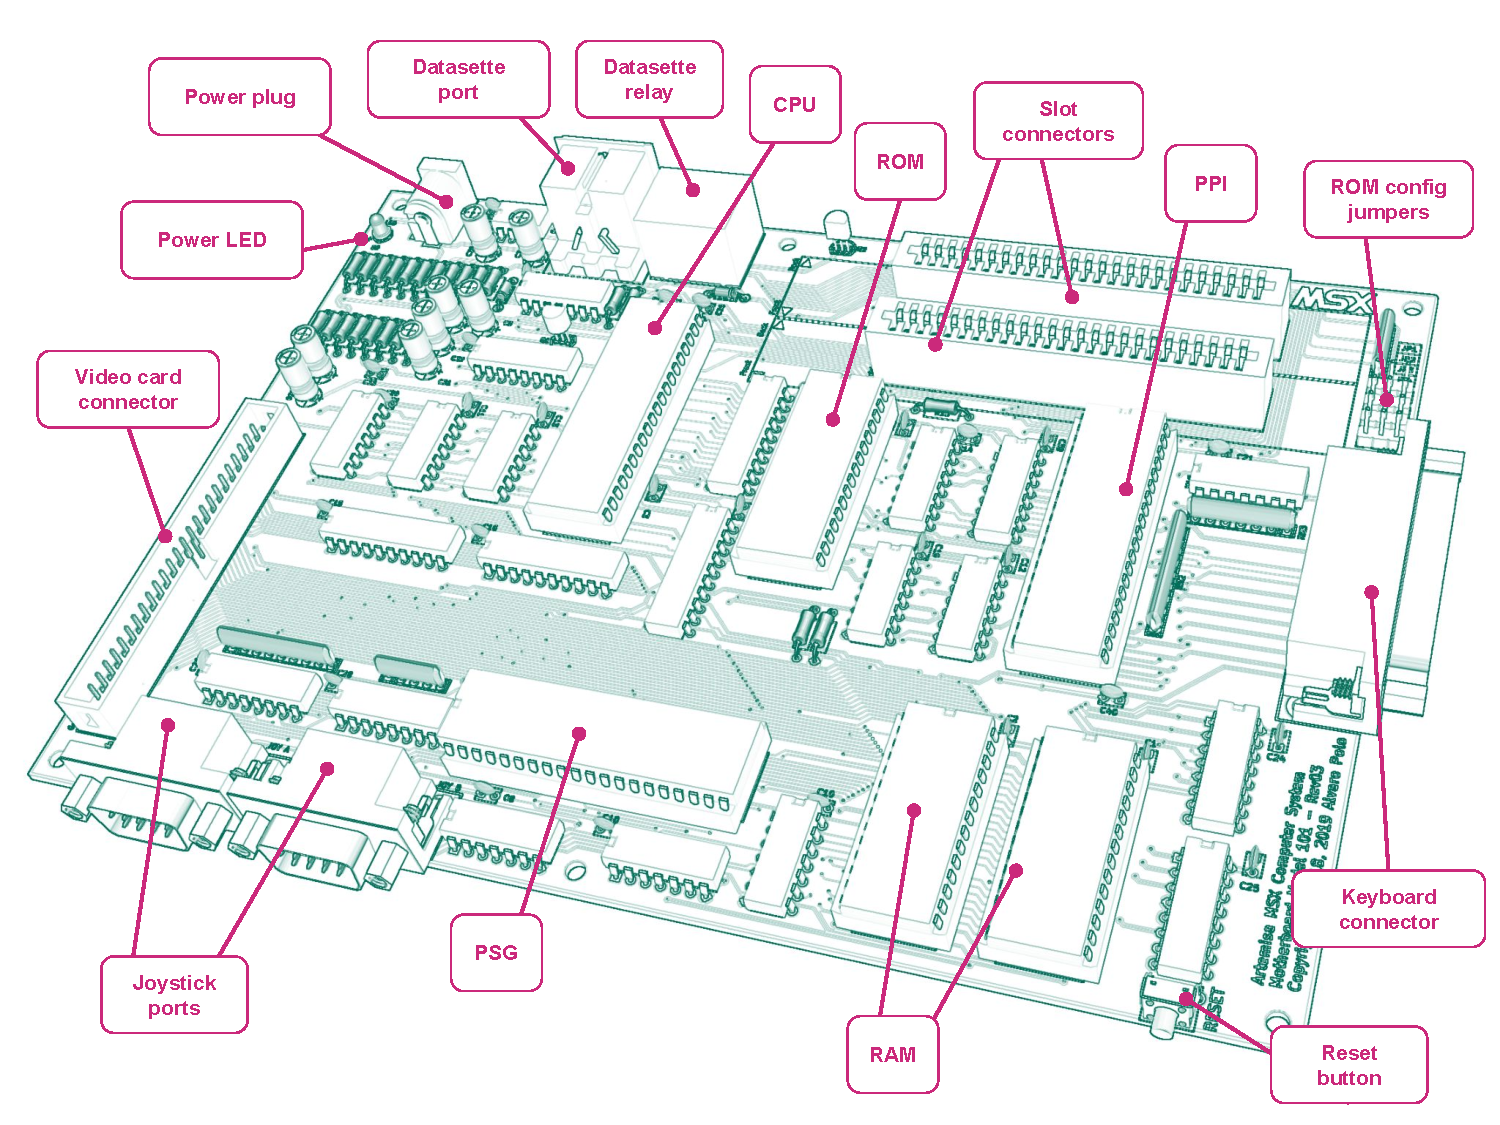
\includegraphics[width=\linewidth]{figures/artemisa-anatomy}
  \caption{Anatomy of the motherboard of an Artemisa computer model 101}
  \label{fig:artemisa-anatomy}
\end{figure}

As you can see, the whole motherboard can be implemented with just 28 integrated circuits, 40 capacitors, 24 resistors, 5 resistor networks, 3 diodes, 2 transistors, 8 connectors, 1 switch, 4 jumpers and 1 crystal oscillator. It will take a few hours to assemble, but its grade of complexity will allow you to understand how an MSX computer works to its most insignificant detail.

It is recommended to observe Figure \ref{fig:artemisa-anatomy} in order to locate the principal components of the motherboard: CPU, RAM and ROM memory, PSG, PPI, etc. But do not bother to memorize it. We will come back to this view when we need it.

Now that you know the high level operation of an Artemisa MSX computer, it is time to prepare for the assembly and discovery process of how it works under the hoods.

\chapter{Preparation}

\section{Contents of the package}

The package Artemisa Computer Model 101 contains the elements described in Table \ref{table:package-contents}:\\

\begin{longtable}{m{10mm}|l}
	\centering
	
\includegraphics{icons/book}          & {\bf Artemisa Computer Model 101 Handbook}                  \\
	                                      &                                                             \\
	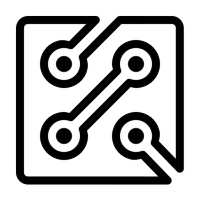
\includegraphics{icons/pcb}           & {\bf Artemisa Motherboard 101 printed circuit board}        \\
	                                      &                                                             \\
	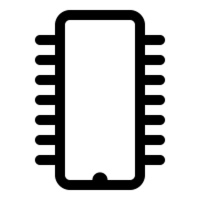
\includegraphics{icons/ic}            & {\bf Integrated circuits ESD bag, including:}               \\
	                                      & 1x Z84C00 CMOS CPU                                          \\
	                                      & 1x 82C55 Parallel Peripheral Interface                      \\			
	                                      & 1x AY-3-8910 Programmable Sound Generator                   \\
	                                      & 2x HM62256/AS62256 32KB SRAM                                \\
	                                      & 1x SST39SF040 512KB flash ROM memory                        \\
	                                      & 1x 74HC04 hex inverter                                      \\
	                                      & 1x 74HCU04 unbuffered hex inverter                          \\
	                                      & 1x 74LS07 open-collector hex buffer                         \\
	                                      & 1x 74HC08 quad 2-input AND gate                             \\
	                                      & 1x 74HCT08 quad 2-input AND gate with TTL-compatible inputs \\
	                                      & 3x 74HC32 quad 2-input OR gate                              \\
	                                      & 2x 74HC74 dual D-type flip flop                             \\
	                                      & 2x 74HC157 quad 2-input multiplexer                         \\
	                                      & 3x 74HC138 3-to-8 line decoder/demultiplexer                \\
	                                      & 1x 74HC139 dual 2-to-4 line decoder/demultiplexer           \\
	                                      & 1x 74HC153 dual 4-input multiplexer                         \\
	                                      & 3x 74HCT244 octal buffer/line driver                        \\
	                                      & 1x 74HCT245 octal bus transceiver                           \\
	                                      & 1x LM311 differential voltage comparator                    \\
	                                      &                                                             \\
	
\includegraphics{icons/conn}          & {\bf Sockets and connectors bag, including:}                \\
	                                      & 2x IC Socket 28p .600 mil                                   \\
	                                      & 1x IC Socket 32p .600 mil.                                  \\
	                                      & 3x IC Socket 40p .600 mil.                                  \\
	                                      & 1x IDC 50p. board connector                                 \\
	                                      & 1x DB25 male board connector                                \\
	                                      & 1x DIN45326 8p. board connector                             \\
	                                      & 2x 50p. edge card connector                                 \\
	                                      & 1x 55x21mm barrel DC connector                              \\
	                                      & 2x DE9 make connector                                       \\
	                                      &                                                             \\
	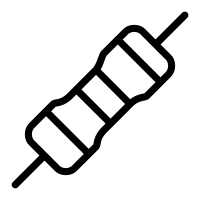
\includegraphics{icons/resistor}      & {\bf Resistors bag, including:}                             \\
	                                      & 1x 100 \si{\ohm} resistor                                   \\
	                                      & 1x 220 \si{\ohm} resistor                                   \\
	                                      & 1x 470 \si{\ohm} resistor                                   \\
	                                      & 3x 1K \si{\ohm} resistor                                    \\
	                                      & 1x 2K2 \si{\ohm} resistor                                   \\
	                                      & 3x 2K7 \si{\ohm} resistor                                   \\
	                                      & 6x 4K7 \si{\ohm} resistor                                   \\
	                                      & 4x 10K \si{\ohm} resistor                                   \\
	                                      & 1x 20K \si{\ohm} resistor                                   \\
	                                      & 1x 100K \si{\ohm} resistor                                  \\
	                                      & 1x 220K \si{\ohm} resistor                                  \\
	                                      & 1x 1M \si{\ohm} resistor                                    \\
	                                      & 2x 10K \si{\ohm} 5p. resistor network                       \\
	                                      & 1x 10K \si{\ohm} 7p. resistor network                       \\
	                                      & 2x 10K \si{\ohm} 9p. resistor network                       \\
	                                      &                                                             \\
	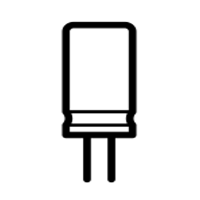
\includegraphics{icons/capacitor}     & {\bf Capacitors bag, including:}                            \\
	                                      & 2x 33pF ceramic capacitor                                   \\
	                                      & 28x 100nF ceramic capacitor                                 \\
	                                      & 2x 22nF ceramic capacitor                                   \\
	                                      & 2x 1uF electrolytic capacitor                               \\
	                                      & 4x 10uF electrolytic capacitor                              \\
	                                      & 2x 100uF electrolytic capacitor                             \\
	                                      &                                                             \\
	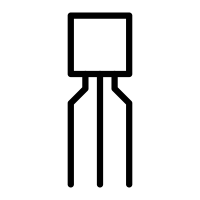
\includegraphics{icons/semiconductor} & {\bf Semiconductors bag, including:}                        \\
	                                      & 2x 1N4448 small signal fast switching diode                 \\
	                                      & 1x 2N2222 NPN bipolar transistor                            \\
	                                      & 1x 2N2907 PNP bipolar transistor                            \\
	                                      & 1x 3mm LED diode                                            \\
	                                      &                                                             \\
	
\includegraphics{icons/misc}          & {\bf Miscellanea components bag, including:}                \\
	                                      & 1x relay 5VDC                                               \\
	                                      & 4x pin header 3p. 100mil                                    \\
	                                      & 4x pin header jumper                                        \\
	                                      & 1x 6x6mm angled push button                                 \\
	                                      & 1x 3.58 MHZ crystal                                         \\
	                                      &                                                             \\
	\caption{Contents of the package}
	\label{table:package-contents}
\end{longtable}

If some part is missing or damaged, please contact {\bf support@artemisamsx.com}.

\section{Required tools}

You will need the tools listed in Table \ref{table:assembly-tools} to assembly your GFX9918 unit:

\begin{longtable}{m{10mm}|m{100mm}}
	\centering
	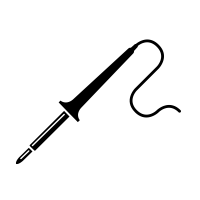
\includegraphics{icons/iron}    & {\bf Electric soldering iron}                                                                                                        \\
	                                & One suitable for soldering electronic components.                                                                                    \\
	                                &                                                                                                                                      \\
	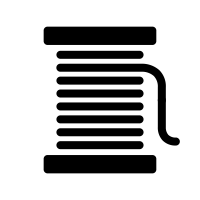
\includegraphics{icons/cable}   & {\bf Spool of solder cable}                                                                                                          \\
	                                & If you have a limited experience on soldering, lead-based alloy is recommended. It melts at lower temperature, facilitating the job. \\
	                                &                                                                                                                                      \\
	
\includegraphics{icons/flux}    & {\bf Soldering flux}                                                                                                                 \\
	                                & A chemical cleaning agent used in the soldering process. Improves the thermal conductivity of the metals, ensuring lasting joints.   \\
	                                &                                                                                                                                      \\
	
\includegraphics{icons/cutters} & {\bf Wire cutters}                                                                                                                   \\
	                                & You will need to remove the remains of legs for resistors and capacitors.                                                            \\
	                                &                                                                                                                                      \\
	\caption{Tools required for assembly}
	\label{table:assembly-tools}
\end{longtable}

The tools listed in Table \ref{table:assembly-opt-tools} may be useful during the assembly process but are not required. If you have access to them, it would be a good idea to prepare them. If not, do not worry. You can assemble your unit without them.

\begin{longtable}{m{10mm}|m{100mm}}
	\centering
	
\includegraphics{icons/multimeter}     & {\bf Multimeter}                                            \\
	                                       & It might be useful to check circuit voltage and continuity. \\
	                                       &                                                             \\
	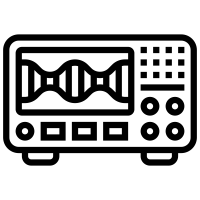
\includegraphics{icons/oscilloscope}   & {\bf Oscilloscope}                                          \\
	                                       & Useful if you want to debug some analog signals.            \\
	                                       &                                                             \\
	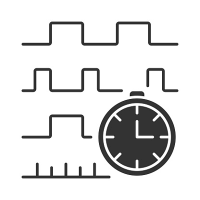
\includegraphics{icons/logic-analyzer} & {\bf Logic analyzer}                                        \\
	                                       & Useful if you want to debug some digital signals.           \\
	                                       &                                                             \\
	\caption{Tools useful but optional for assembly}
	\label{table:assembly-opt-tools}
\end{longtable}



\chapter{Power and Reset}

\section{Circuit description}

The figure \ref{fig:artemisa-schematic-power} shows the schematic diagram of the power management and power-on reset circuits.

\begin{figure}[htbp]
  \centering
  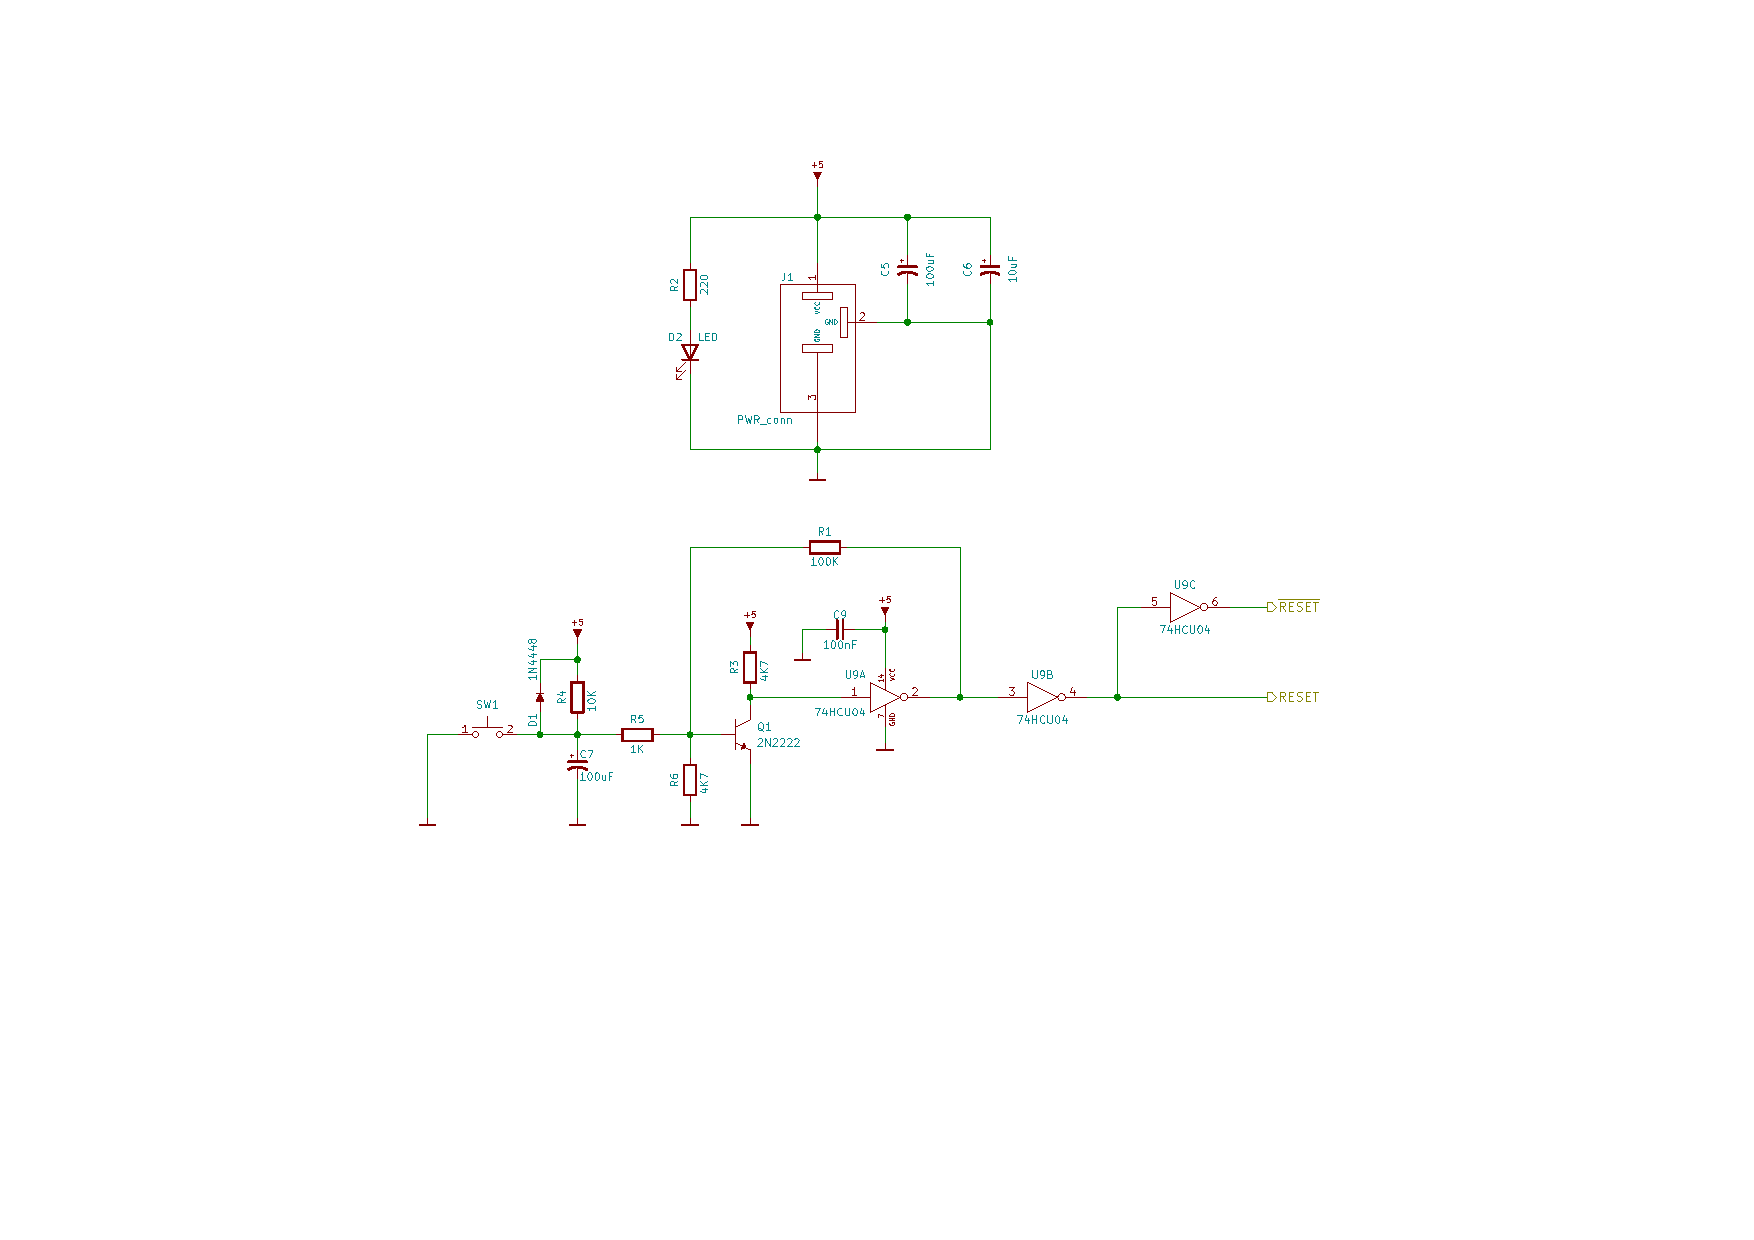
\includegraphics[width=\linewidth,trim={6cm 7cm 6cm 2.5cm},clip]{figures/artemisa-schematic-power}
  \caption{Schematic diagram of power input and power-on reset}
  \label{fig:artemisa-schematic-power}
\end{figure}

As you can see, the schematic sheet is divided in two separated blocks.

\begin{itemize}
  \item At the top side of the schematic we have the power connector circuit. This shows the circuit formed by the DC power barrel connector and a few auxiliary elements around it.
  \item At the bottom side of the schematic we have the power-on reset circuit. This contains the reset button and several components aimed to generate a reset signal to get several computer devices to their initial state.
\end{itemize}

We will analyze each subcircuit separately.

\subsection{Power connection}

Starting with the power connector. This is extremely simple, as shown in \ref{fig:artemisa-schematic-power-conn}. The DC barrel connector {\tt J1} provides three different terminals: 1, 2 and 3. 1 is the positive input terminal, or {\tt VCC}. 2 and 3 are the negative input terminals, or {\tt GND}. As you can see, they are directly connected to the {\tt +5} and {\tt GND} power symbols, respectively. This means the DC barrel connector is feeding the five volts and the ground inputs. Whenever we see the {\tt +5} and {\tt GND} power symbols in the schematic, we know they are wired to and powered from the {\tt J1} connector.

\begin{figure}[htbp]
  \centering
  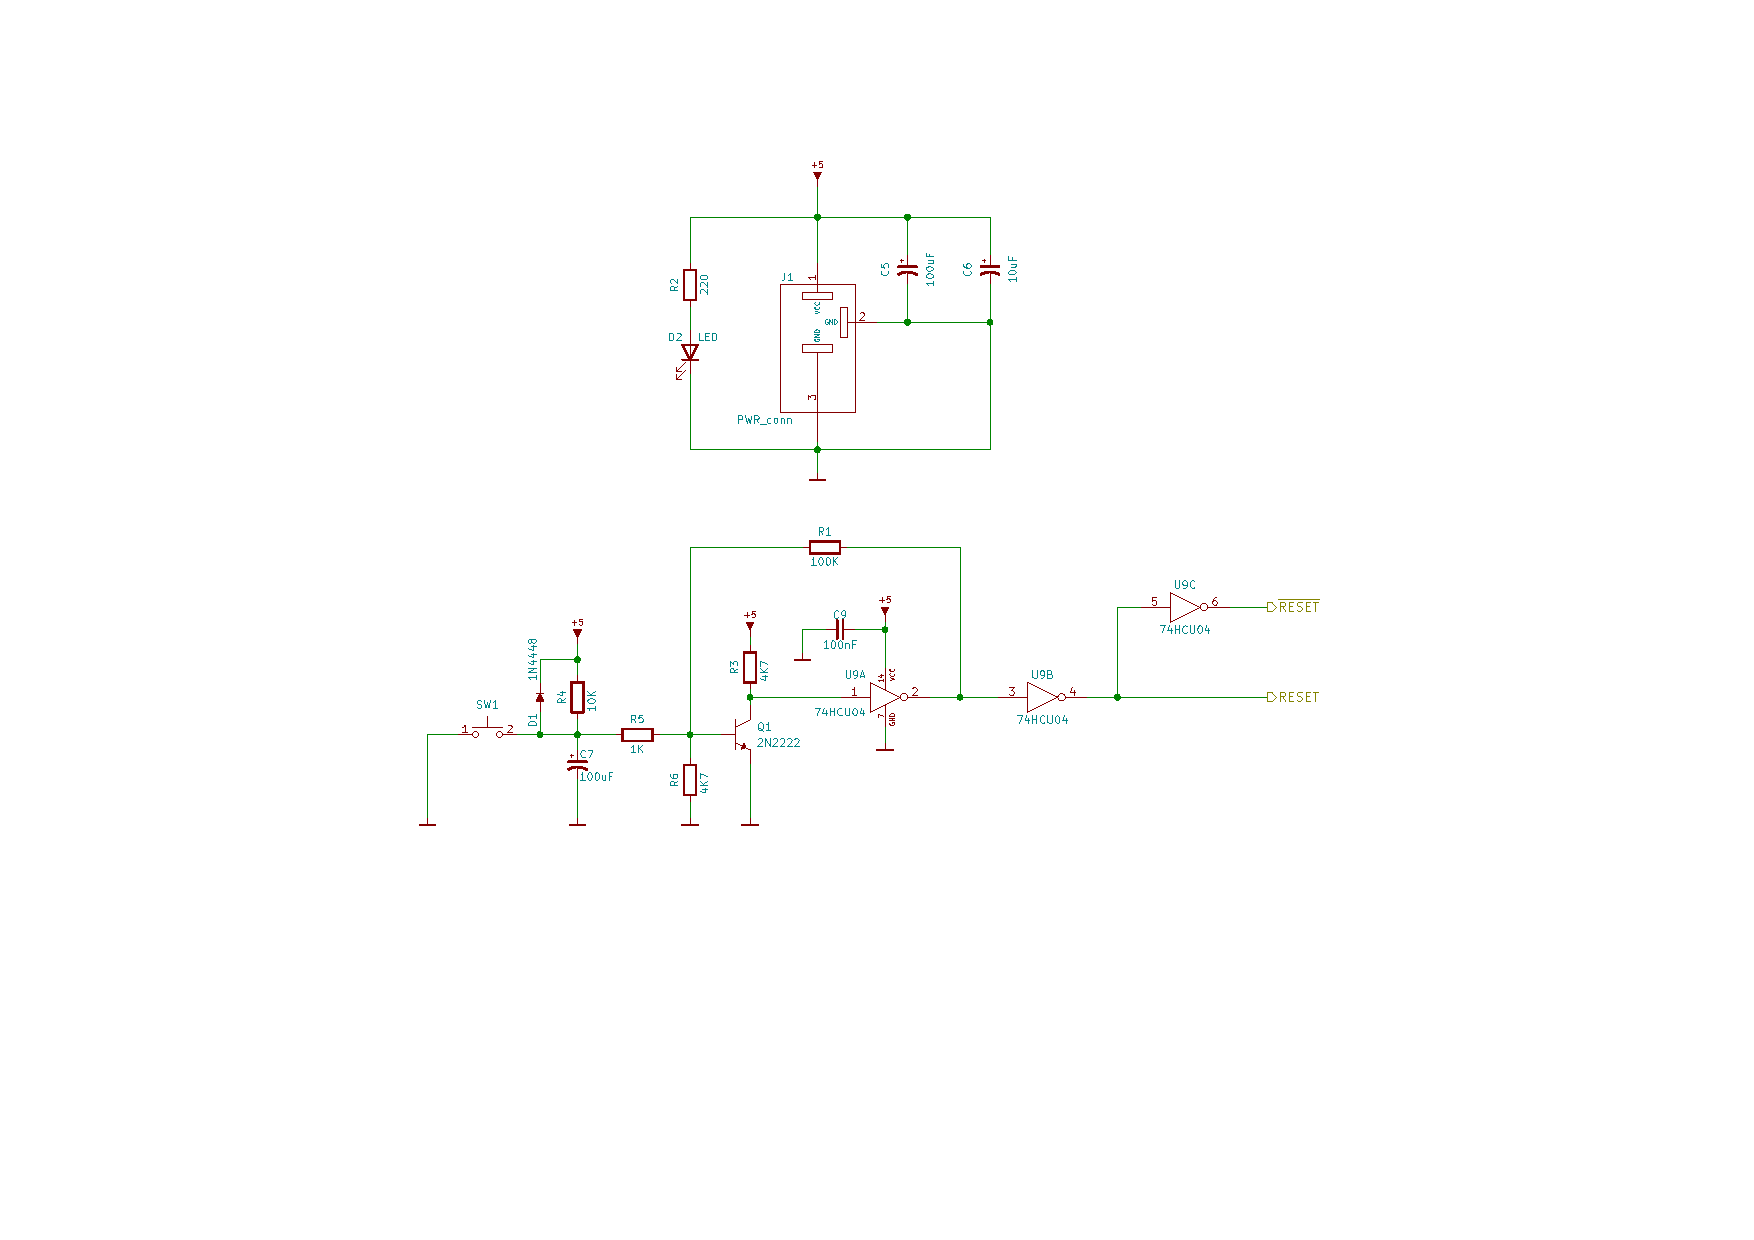
\includegraphics[width=0.5\linewidth,trim={11cm 12.8cm 12.4cm 2.5cm},clip]{figures/artemisa-schematic-power}
  \caption{Schematic diagram of power connector}
  \label{fig:artemisa-schematic-power-conn}
\end{figure}

The LED \toref{diode} {\tt D2} is used to indicate the computer is powered on when the power cable is connected to {\tt J1}. The resistor {\tt R2} is used to limit the current passing throught {\tt D2}.

\begin{theory}[htbp]{Diodes}
  Diodes are semiconductor devices that conduct the electric current only in one direction. They have two terminals: the anode and the cathode. The current flows from the anode to the cathode (forward current), but never from the cathode to the anode (reverse current). The forward current experiments a voltage drop of a few volts caused by the junction of semiconductor material in the diode, typically of 0.6-0.7 volts.\\\\

  LEDs, or light-emitting diodes, are a special kind of diodes that emits light when forward current flows through it. Their voltage drop depends on the color of the light they emit, and it is typically of a few volts. Apart from this particularity, their behavior is the same as any other type of diode.\\\\

  Any diode, LEDs included, does not offer any resistance to the forward current. The current experiments a voltage drop as discussed above. But once that voltage drop is exceeded, all the current will flow following the Ohms law. This means that, in the absence of any other kind of resistor in the circuit, the current will be theorically infinite (as $I = \frac{V}{R}\), when $R\) is zero). Or, in other words, a short-circuit will happen.\\\\

  For that reason, LEDs are always put in series with a resistor that will limit the current that traverses the circuit. Otherwise, we will have a short-circuit that will destroy the LED, and could damage the power supply.
\end{theory}

You can also find two large electrolytic capacitors: {\tt C5} and {\tt C6}. They are \toref{decoupling capacitors} used to filter the voltage fluctuations that may occur in the power adapter connected to {\tt J1}.

\begin{theory}[htbp]{Decoupling capacitors}
  Integrated circuits do not consume an even electric current. They experiment fluctuations. They work like a building. If many occupiers open their water taps, the whole building will demand a high flow of water from the external water supply. If most of them close their taps, the flow will be low. Integrated circuits are made of transistors. And each transistor is equivalent to a water tap. They are open or closed depending on their inputs and their previous states.\\\\

  When part of the circuit experiments a spike in their current demand, the power supply must satisfy it. However, power supplies are not ideal. They will try to adequate the supplied voltage to the new demands. But it does not happen immediately. As result, some parts of the circuit could experiment a brief voltage drop. This can have effects to the integrated circuits, generating errors like misinterpreting digital input values.\\\\

  The way to prevent this is to use decoupling capacitors. They will act as local batteries connected to some part of the circuit. If there is any voltage drop in the power input, the charge of the capacitor will compensate the lost. The capacitor will operate as a power supply for a short period of time (while it is charged), ensuring the voltage level is even regardless the fluctuations in the supply and the demand. In the building analogy, this is like putting a water tank at the input pipe of the building. All occupiers can open their taps all at once. The tank will feed the taps while the water supplier adapts the flow to the new demand.\\\\

  Typically, every integrated circuit has its own small decoupling capacitor to protect it from the voltage fluctuations. There are also some bulk capacitors aimed to decouple the whole power circuit of the board from the power line coming from the DC barrel connector.
\end{theory}

\subsection{Power-On Reset}

The second part of the schematic sheet shown in figure \ref{fig:artemisa-schematic-por} is the power-on reset circuit. This part is by far more complex than the power connector part. And also more complex than most of the circuits we will analyze in this book. So we will explain how it works with an analysis of how the current flows on power on and how it affects the \sym{RESET} and \sym{/RESET} outputs.

\begin{figure}[htbp]
  \centering
  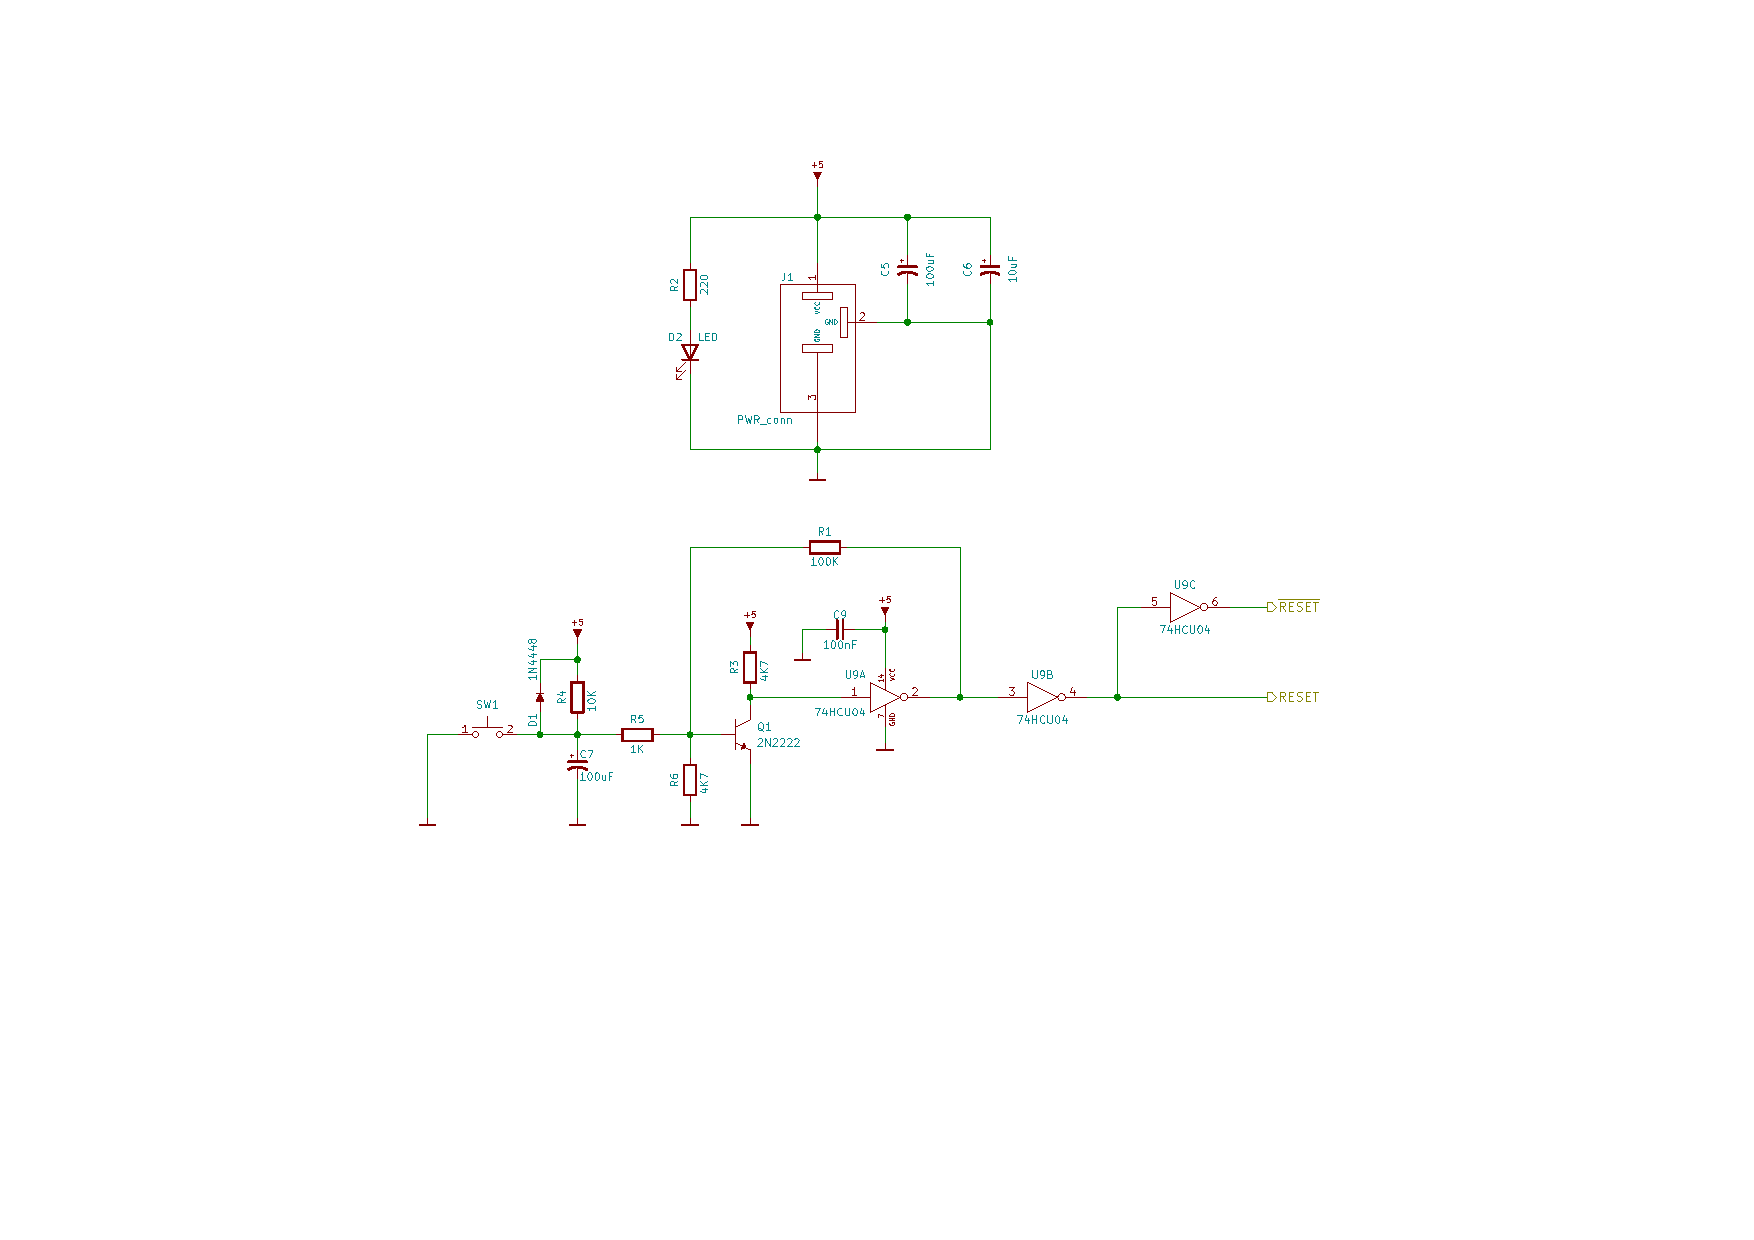
\includegraphics[width=\linewidth,trim={6cm 7cm 6cm 8.5cm},clip]{figures/artemisa-schematic-power}
  \caption{Schematic diagram of power-on reset circuit}
  \label{fig:artemisa-schematic-por}
\end{figure}

We will start assuming we just have connected the power cable to the DC barrel connector. This situation is represented by the simulation shown in Figure \ref{fig:simul-por-01}.

\begin{figure}[htb]
  \centering
  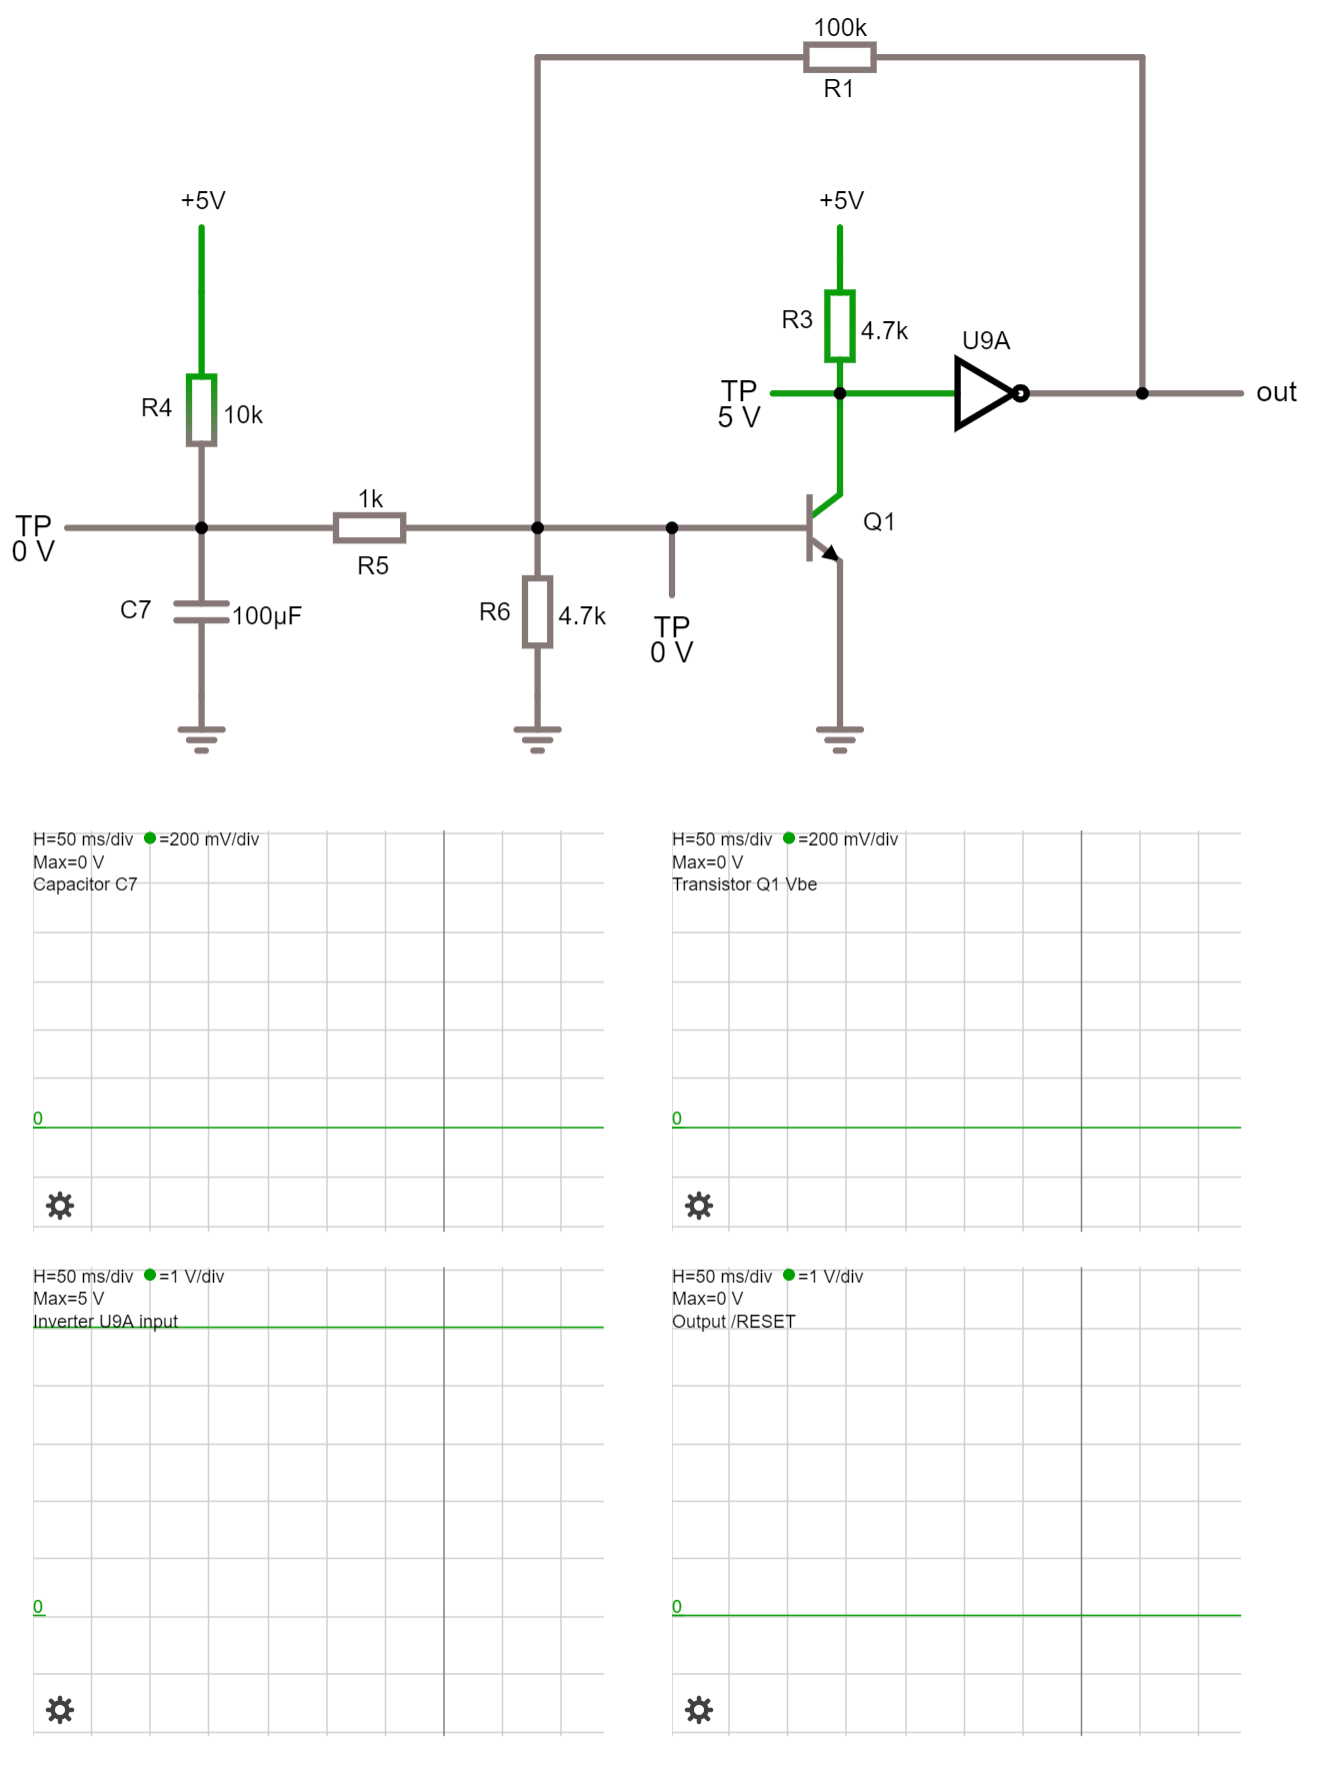
\includegraphics[width=0.7\linewidth]{figures/simul-por-01}
  \caption{Simulation of Power-On Reset: initial state after power on}
  \label{fig:simul-por-01}
\end{figure}

In that instant, the current is ready to flow from the {\tt +5} power supply throught {\tt R4} to reach the positive terminal of the capacitor {\tt C7}. We will assume this capacitor is discharged because the circuit was not energized yet. So the voltage in its positive terminal is initially zero.

As the voltage in {\tt C7} is almost zero, there is almost no current flowing through {\tt R5} or {\tt R6} to the base terminal of \toref{transistor} {\tt Q1}. Thus, the transistor will operate in the cut-off region.

As the transistor is cut-off, its collector-emitter junction is equivalent to an open circuit without any current flowing through the collector terminal. Thus, the 5 volts across {\tt R3} are \toref{transmitted to the input terminal} of the 74HCU04 logic inverter {\tt U9A}. These 5 volts are represented in the simulation circuits like Figure \ref{fig:simul-por-01} with green coloured wires that are turned into grey as their voltage drops to zero.

\begin{theory}[htbp]{Transistors}
  Transistors are semiconductor devices used to amplify or switch electronic signals. They have three terminals. The voltage level between a pair of these terminals determine the current through another pair of terminals. The power of the controlled output can be higher than the power of the controller input. Thus, they can amplify a electric signal.\\\\

  In this particular example of figure \ref{fig:artemisa-schematic-por}, we are using a NPN bipolar transistor for switching purposes. These transistors have three terminals known as base (left), emitter (below, with an arrow) and collector (above). The current between base and emitter ($I_B$) determines the current that will go from the collector to the emitter ($I_C$).\\\\

  \begin{itemize}
    \item When the voltage at the base terminal is low, there will be no current from the base to the emitter. Thus, the transistor will be cut-off and no current will flow. The collector-emitter junction will be equivalent to an open circuit.
    \item If the voltage at the base terminal is high, the transistor will saturate and will let pass as much current as possible from the collector to the emitter. The collector-emitter junction will be equivalent to a closed circuit.
  \end{itemize}
\end{theory}

\begin{theory}[htbp]{Voltage drop when current is zero}
  Perhaps you might wonder why the input terminal of {\tt U9A} has 5 volts when {\tt Q1} is cut-off considering there is a resistor {\tt R3} in the path. The aswer to this is given by the Ohms law.\\\\

  As {\tt Q1} is cut-off, there is only one possible path for the current: from {\tt 5+} to the input terminal of the logic inverter {\tt U9A}. The logic inverter, as any other logic gate, has a huge input impedance around 6M\si{\ohm}. This means the current going through the logic gate input terminal is almost zero. The voltage in the input terminal of {\tt U9A} is the five volts from the power supply minus the voltage drop in {\tt R3}, or $V_{in} = 5v - V_{R3}$. If there is no current, the Ohms law $V=I \cdot R$ reveals the voltage drop $V_{R3}$ is zero. Thus, the voltage at the input terminal of the logic gate is 5 volts.\\\\

  The rule of thumb is that, in the absence of current due to very high impedances, the voltage remains constant in all those points where current is not flowing. No matter the resistors we put on its way.
\end{theory}

As the logic inverter {\tt U9A} receives 5v in its input, or a high level in the digital world, it generates 0v in the output, a low level. That is the out point shown in Figure \ref{fig:simul-por-01}. We could be considered our active-low reset signal. However, it is a good idea to isolate this part of the circuit from the rest of devices that will use the output.

This isolation is done by using {\tt U9B} and {\tt U9C} as buffers. The logic gate {\tt U9B} shown in Figure \ref{fig:artemisa-schematic-por} inverts the output from {\tt U9A}  again, producing a signal labeled as {\tt RESET} whose logic value is high at this instant. {\tt U9C} inverts that signal one more time to generate {\tt /RESET}, the active-low reset signal, which will be low at this point in time.

After this analysis, we can be sure the reset pulse will initiate upon power adapter is plugged into the DC barrel connector. This is represented in the graphs and test points shown in Figure \ref{fig:simul-por-01}. After that instant zero, some milliseconds will pass while the current from the power supply is flowing through {\tt R4} to the input terminal of the capacitor. This is represented by the simulation shown in Figure \ref{fig:simul-por-02}.

\begin{figure}[htb]
  \centering
  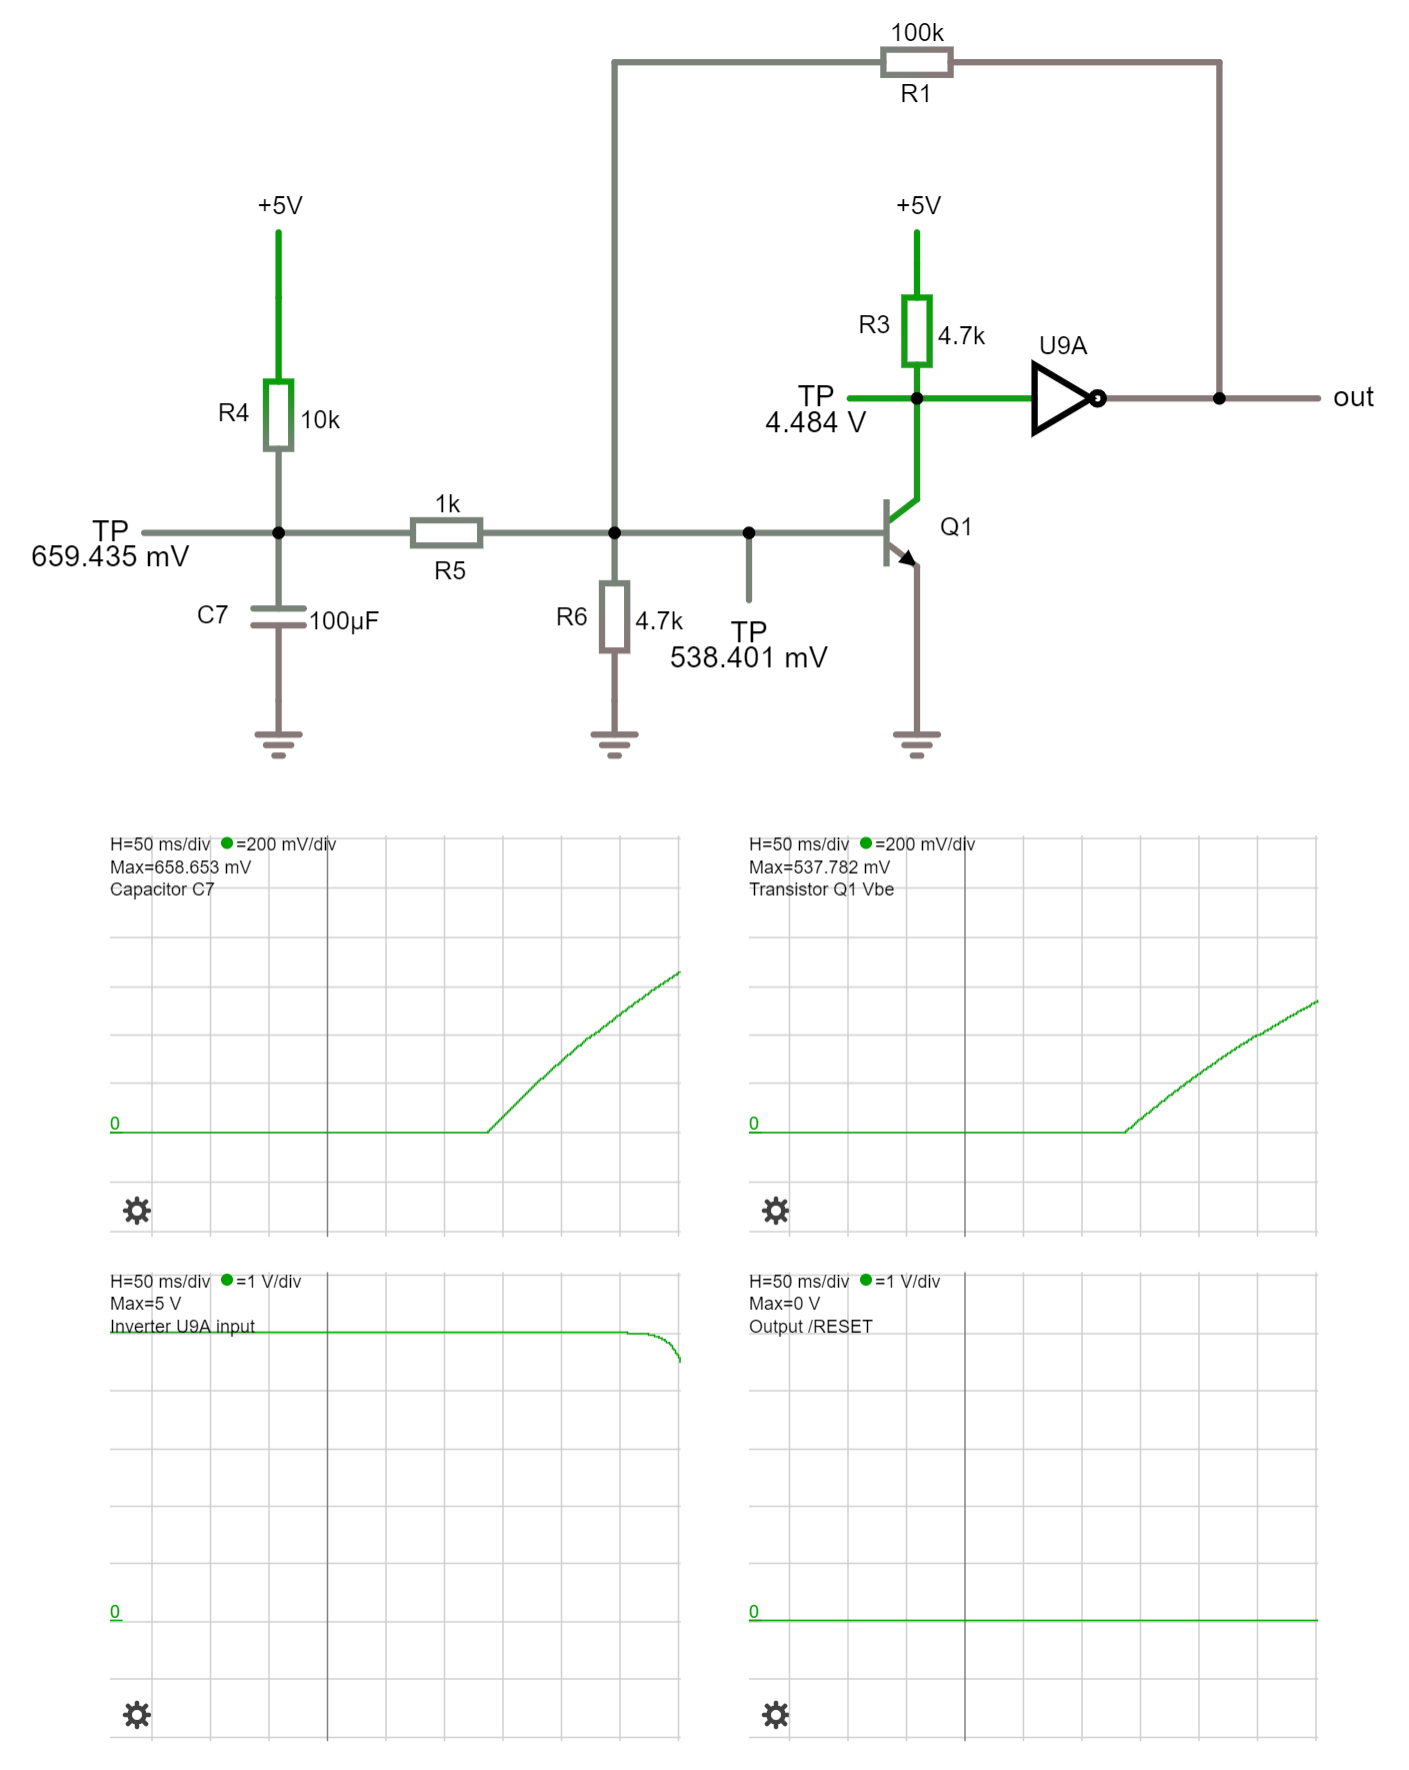
\includegraphics[width=0.7\linewidth]{figures/simul-por-02}
  \caption{Simulation of Power-On Reset: the capacitor {\tt C7} initiates its charge cycle}
  \label{fig:simul-por-02}
\end{figure}

As the current is flowing, it will initiate the charging cycle of the capacitor, what requires some time to complete. During that time, it will be draining the current coming from the power supply throught {\tt R4}. And the voltage in its positive terminal will increase slowly, following a loading curve shown in the top-left graph of the simulation in Figure \ref{fig:simul-por-02}.

As the time passes, the capacitor will increase its charge and voltage. And that will also increase the current going through {\tt R5} and {\tt R6}. Part of this current will go through the base terminal of the transistor {\tt Q1}, making it leave the cut-off region to enter the active region. This is shown in the top-right graph of the simulation in Figure \ref{fig:simul-por-02}.

When this happens, the collector-emitter current will be the base current amplified by the transistor gain: $I_C = h_{FE} \cdot I_B$. This will cause a voltage drop in {\tt R3} due to that current, with an interesting side effect: the voltage at the input terminal of {\tt U9A} will be reduced. This is shown in the bottom-left graph of the simulation in Figure \ref{fig:simul-por-02}.

At this moment, the collector current is still too low to cause a significant voltage drop in {\tt R3}. Thus, the voltage at the input of {\tt U9A} is still above the transition level. As consequence, the output of {\tt U9A} is still low. This is shown in the bottom-right graph of the simulation in Figure \ref{fig:simul-por-02}.

So in summary, the voltage of the input terminal of {\tt U9A} is inversely proportional to the charge of the capacitor {\tt C7}. The more charge in the capacitor, the less voltage in the logic inverter.

Approximately 100ms after power on, the situation changes to that represented in the simulation shown in Figure \ref{fig:simul-por-03}.

\begin{figure}[htb]
  \centering
  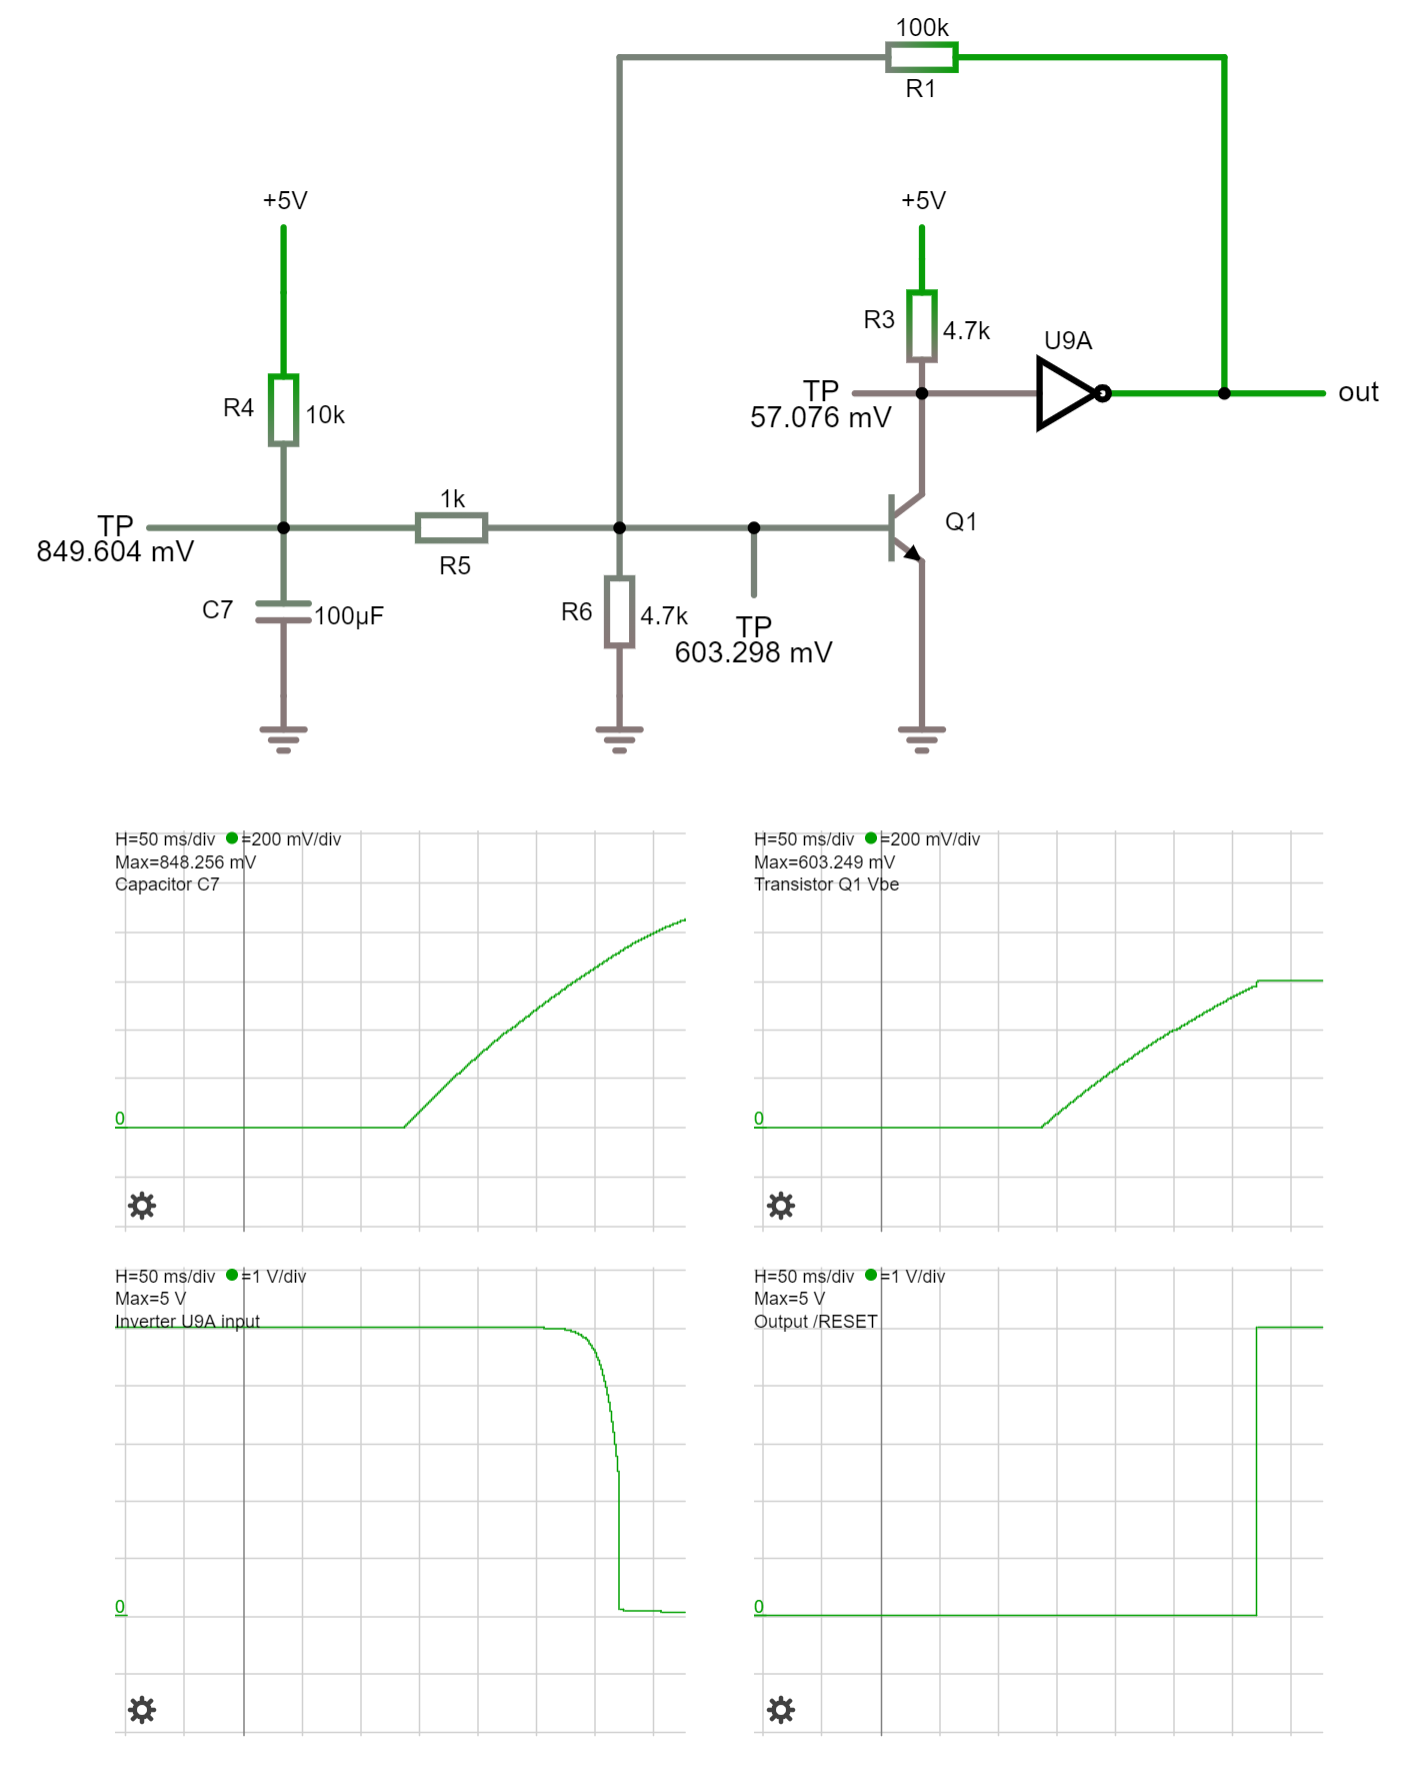
\includegraphics[width=0.7\linewidth]{figures/simul-por-03}
  \caption{Simulation of Power-On Reset: the charge of {\tt C7} causes a transition in {\tt U9A}}
  \label{fig:simul-por-03}
\end{figure}

The charge in {\tt C7} has been increased following its charge curve. This is shown in the top-left graph of the simulation of Figure \ref{fig:simul-por-03}.

As consequence, the transistor {\tt Q1} pushes more and more current through its collector. This is shown in the top-right graph of the simulation of Figure \ref{fig:simul-por-03}.

The collector current in the transistor causes a voltage drop in {\tt R3} that reduces the voltage at the input of {\tt U9A} below the transition level. This is shown in the bottom-left graph of the simulation of Figure \ref{fig:simul-por-03}.

Once the input of {\tt U9A} falls below some mid-point level, the inverter will transit into a new state. The output will change from logic low to high. This is shown in the bottom-right graph of the simulation of Figure \ref{fig:simul-por-03}.

The rest of inverters {\tt U9B} and {\tt U9C} will change their state as well. So the level of {\tt RESET} will pass to be low and the level of {\tt /RESET} will pass to be high. That is the effective termination of the reset pulse.

However, that is not all. If you look carefully the graphs in Figure \ref{fig:simul-por-03}, you may find something odd. The voltage at the input of {\tt U9A} falls abruptly to zero just after it reaches the mid-point where level transition occurs. In turn, there is also a drastic increment in the $V_{BE}$ of the transistor just before it reaches its top.

This effect is caused by the resistor {\tt R1}. This is a positive feedback loop that connects the output of {\tt U9A} to the base terminal of {\tt Q1}. And there is a good reason to make this. In fact, the Power-On Reset will not work without it!

When input voltage of an inverter is close to the mid-point, any small change in that input will be reflected with a huge change in the output. This is the point where voltage gain is maximum. Unfortunately, any electric wire has some amount of electrical noise that may cause small changes in its voltage, both positive and negative. When this happens in the input of the inverter when the voltage is close to the mid-point, the output could experiment huge oscillations.

This situation is represented in the simulation shown in Figure \ref{fig:simul-por-04}. This time we have altered the simulation to use a noisy power supply instead of perfectly unaltered 5 volts as before. We have also removed the positive feedback loop.

\begin{figure}[htb]
  \centering
  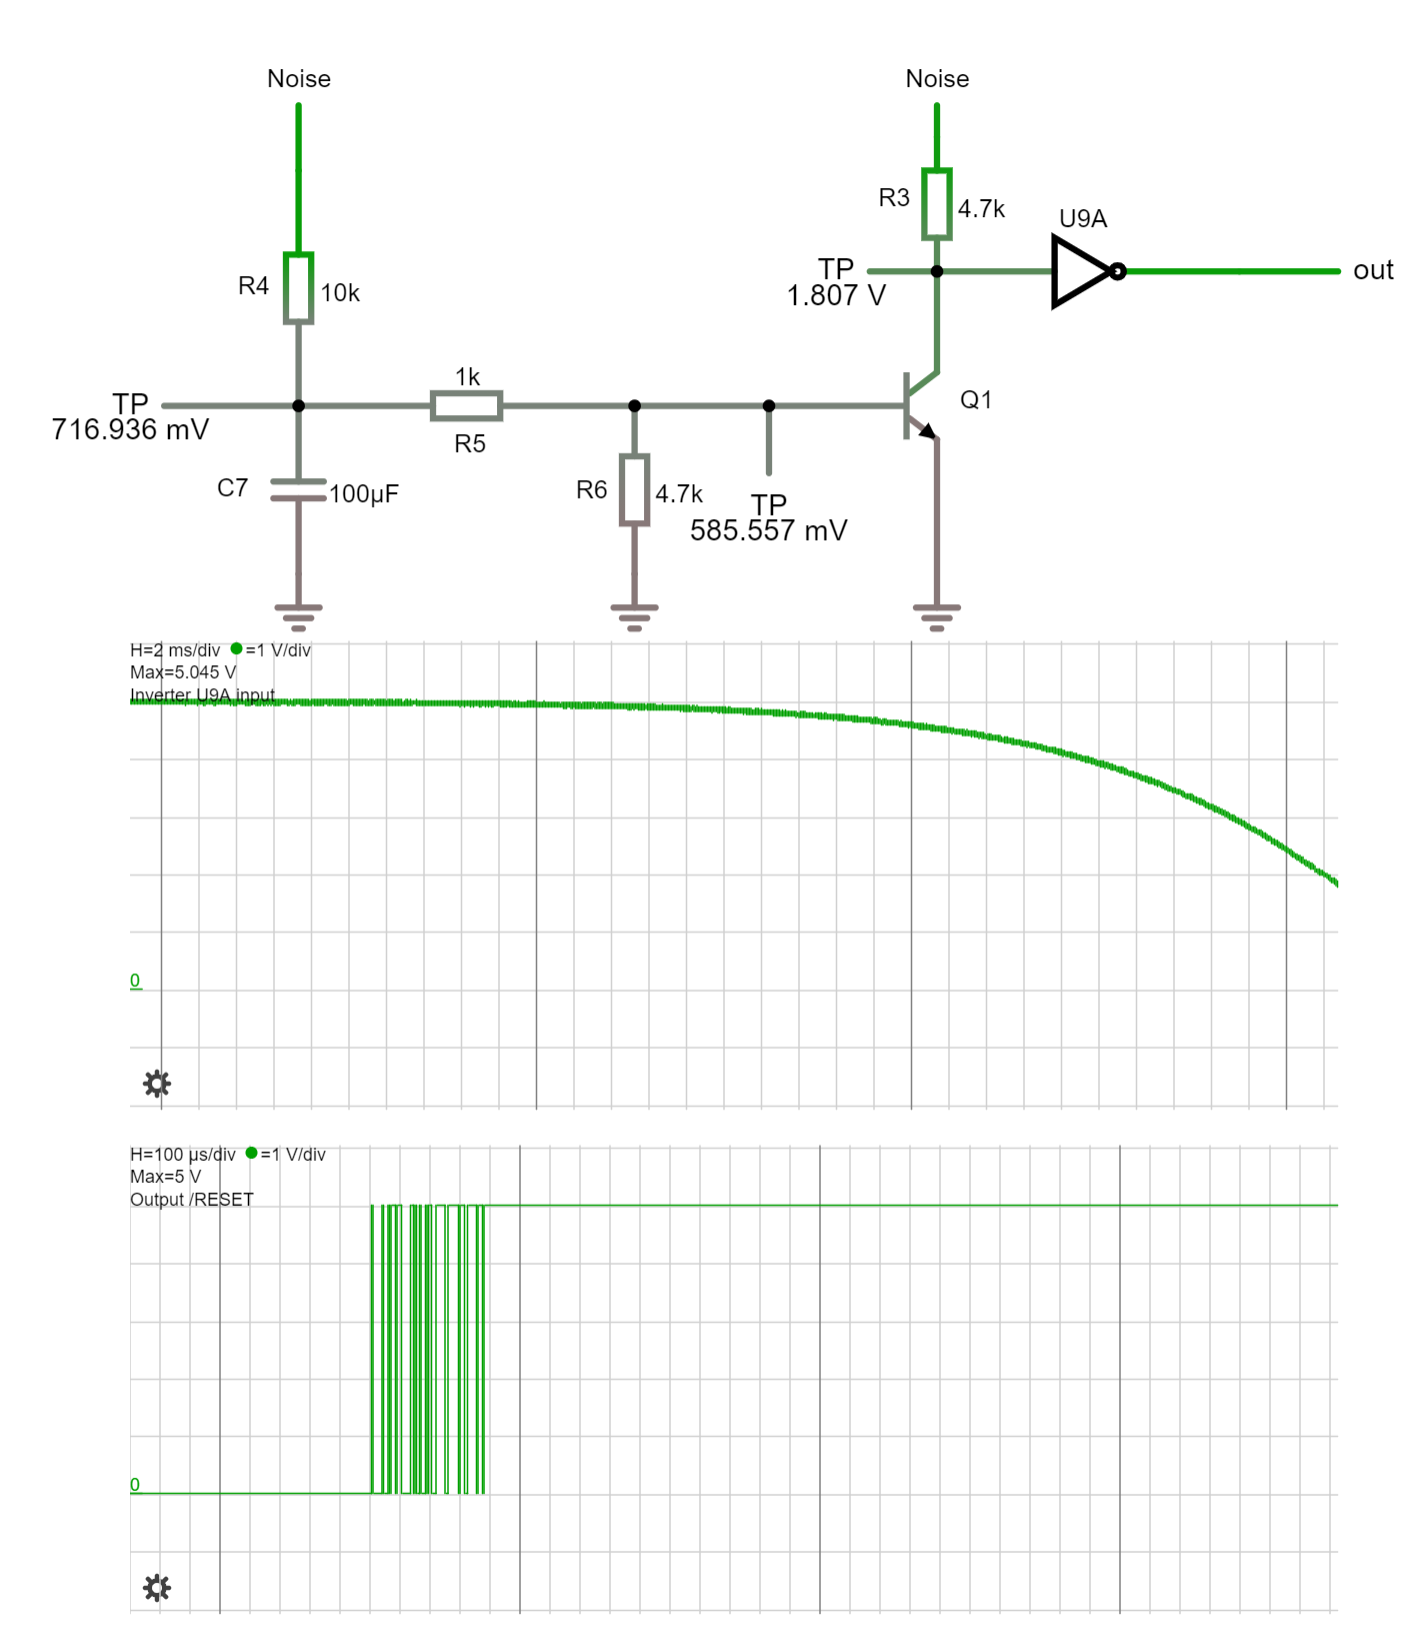
\includegraphics[width=0.7\linewidth]{figures/simul-por-04}
  \caption{Simulation of Power-On Reset: effect of removing the positive feedback loop}
  \label{fig:simul-por-04}
\end{figure}

As we can see in Figure \ref{fig:simul-por-04}, when the input voltage at {\tt U9A} reaches the mid-point (top graph), the noise in the line causes a few oscillations in the output (bottom graph). These oscillations would be interpreted by devices receiving the reset signal as a new reset action. However, they are too short in time. Just a few microseconds in the best case. Some devices as the Z80 CPU requires reset pulses of several milliseconds at minimum. This short and false pulses will left these devices into an inconsistent state. And your computer will not boot correctly.

In a standard logic circuit, this is not an issue due to how fast the signals transit between logic levels. Logic gates are made of transistors that do not respond immediately to the changes in their inputs, taking several nanoseconds to raise or fall one single volt in the output. Thus, if the input signal transition is in the range of nanoseconds, a small noise in the line will not be reflected.

However, in out circuit the input of {\tt U9A} changes very slowly. We can see in the simulation of Figure \ref{fig:simul-por-04} that it takes 40ms just to go from the top of voltage to the mid-point. This is what is known as a slow signal, and it will cause oscillations if they are not handled as we do with the positive feedback loop.

But, how the positive feedback loop is helping to remove the output oscillations? Easy. You can see how it happens in the simulation shown in figure \ref{fig:simul-por-05}.

\begin{figure}[htb]
  \centering
  \includegraphics[width=0.7\linewidth]{figures/simul-por-05}
  \caption{Simulation of Power-On Reset: impact of positive feedback loop in $I_B$ of {\tt Q1}.}
  \label{fig:simul-por-05}
\end{figure}

The first transition from low to high in the output of {\tt U9A} will drive a small current through {\tt R1}. Part of this current will join to the current coming from {\tt R5} to increase the $I_B$ of the transistor. And this increment is not small, as shown in bottom graph of Figure \ref{fig:simul-por-05}. It goes from 5 to 32 microamperes. This current is enough to put the transistor in the saturation region. What means an effective closed circuit between the collector and the emitter. This is what pulls the input voltage of {\tt U9A} to almost zero before the noise has time to cause any oscillation in the inverter.

There is some other thing in this circuit that also helps to mitigate the oscillations in the inverter. This is the usage of a {\tt 74HCU04} inverter instead of {\tt 74HC04}. That extra {\it U} in the part name means {\it unbuffered}.

One of the multiple particularities of unbuffered gates is that they have lower gains than their buffered equivalents. Unbuffered gates have a single amplifier phase, while buffered ones typically have three. Each phase increases the gain of the overall circuit. Thus, you might expect that unbuffered inverters have a maximum gain of a few hundreds, while buffered devices have several thousands.

Higher gain means they will react more drastically to the changes in their inputs. A tiny change in the input voltage caused by line noise will be reflected by an increment several orders of magnitude larger if the inverter is buffered. In other words, buffered gates are more sensible to line noise, specially when slow signals are used. Thus, this design uses {\tt 74HCU04} unbuffered inverters.

Now you know almost everything about a reliable Power-On Reset circuit. Everything but how an actual reset without a power-on can be done. This is achieved by switch {\tt SW1} and a diode {\tt D1} shown at the left side of the circuit of Figure \ref{fig:artemisa-schematic-por}.

The diode is used to discharge the capacitor {\tt C7} quickly when the power is disconnected. When that happens, the {\tt 5+} power will not drive 5 volts any longer, and it can drain the charge of the capacitor going through {\tt D1}. If this diode is not present, it would be possible to disconnect the power adapter and connect it again fastly. Fast enough to maintain the charge of the capacitor, and not having any reset signal. Thanks to the diode, the capacitor {\tt C7} is discharged very quickly as soon as the power adapter is unplugged from the DC barrel connector.

However, having to reconnect the power adapter everytime we want to reset the system is annoying. To avoid this pain in the ass, we have the switch {\tt SW1}. This switch connects the positive terminal of capacitor {\tt C7} to ground. When unpressed, this circuit is open. Upon press, the capacitor will discharge very quickly. This will return to the same state we had when the system was powered on. And a new reset pulse will begin.

Now we can say that is all. You have far enough to understand how the power connector and power-on reset circuits work. It is time to heat up the solder iron.

\section{Circuit assembly}

\subsection{Power connector}

We will start assembling the parts of the power connector circuit shown in Figure \ref{fig:artemisa-schematic-power-conn}.

\begin{enumerate}
  \item Solder the barrel power connector {\tt J1}. Its exact placement is shown in Figure \ref{fig:mount-power-01}.
  \item Solder the decoupling capacitors {\tt C5} and {\tt C6}. Their exact placement is shown in Figure \ref{fig:mount-power-02}.

        \begin{warning}[Be careful with the polarity of the electrolytic capacitors!]
          These capacitors are electrolytic, and they have a polarity. Please check you are soldering the right pads into the right holes. The long pad of the capacitor is the positive terminal. The short pad, which is also marked with a grey mark with minus symbols on the capacitor body, is the negative terminal.\\\\

          Soldering electrolytic capacitors with a reverse polarity may cause them to explode!
        \end{warning}
  \item Solder the resistor {\tt R2} and the LED {\tt D2}. Their exact placement is shown in Figure \ref{fig:mount-power-03}. Take care of the polarity of the LED. The long pad is the anode, and must be soldered in the hole with the plus sign mark. The short pad, which also have a notch in the base of the LED body, is the cathode, and must be soldered in the hole marked with the minus sign.
\end{enumerate}

\begin{figure}[htbp]
  \centering
  \includegraphics[width=0.8\linewidth]{figures/mount-power-01}
  \caption{Placement of power barrel connector {\tt J1}}
  \label{fig:mount-power-01}
\end{figure}

\begin{figure}[htbp]
  \centering
  \includegraphics[width=0.8\linewidth]{figures/mount-power-02}
  \caption{Placement of decoupling capacitors {\tt C5} and {\tt C6}}
  \label{fig:mount-power-02}
\end{figure}

\begin{figure}[htbp]
  \centering
  \includegraphics[width=0.8\linewidth]{figures/mount-power-03}
  \caption{Placement of resistor {\tt R2} and the LED {\tt D2}}
  \label{fig:mount-power-03}
\end{figure}

Once all the parts from the power circuit are assembled, it is time to test it:

\begin{enumerate}
  \item Connect the power adapter cable to the DC barrel connector. If everything goes well, the power LED will illuminate.
  \item If you have a multimeter, you can measure the DC voltage between the positive and negative terminals of the barrel connector. They should indicate a typical value of 5.00 volts. Any value from 4.75 to 5.25 volts is correct.
  \item Try to disconnect the power adapter cable. You will see the power LED is still illuminated. This is because the capacitors {\tt C5} and {\tt C6} are charged and they are feeding the LED. After a few seconds, the power drained by the LED circuit will discharge the capacitors and the LED will fade.
\end{enumerate}

\subsection{Power-On Reset}

Now we have the power sources assembled, it is time to go with the Power-On Reset circuit described in Figure \ref{fig:artemisa-schematic-por}.:

\begin{enumerate}
  \item Solder the resistors {\tt R4}, {\tt R5}, {\tt R6} and {\tt R1}. Their exact placement is shown in Figure \ref{fig:mount-power-04}.
  \item Solder the capacitor {\tt C7}. Its exact placement is shown in Figure \ref{fig:mount-power-05}.
  \item Solder the diode {\tt D1}. Its exact placement is shown in Figure \ref{fig:mount-power-06}.
  \item Solder the transistor {\tt Q1}. Its exact placement is shown in Figure \ref{fig:mount-power-07}.
  \item Solder the reset push button {\tt SW1}. Its exact placement is shown in Figure \ref{fig:mount-power-08}.
  \item Solder the IC {\tt U9} and its decoupling capacitor {\tt C9}. Their exact placement is shown in Figure \ref{fig:mount-power-09}.
\end{enumerate}

\begin{figure}[htbp]
  \centering
  \includegraphics[width=0.8\linewidth]{figures/mount-power-04}
  \caption{Placement of resistors {\tt R4}, {\tt R5}, {\tt R6} and {\tt R1}}
  \label{fig:mount-power-04}
\end{figure}

\begin{figure}[htbp]
  \centering
  \includegraphics[width=0.8\linewidth]{figures/mount-power-05}
  \caption{Placement of capacitor {\tt C7}}
  \label{fig:mount-power-05}
\end{figure}

\begin{figure}[htbp]
  \centering
  \includegraphics[width=0.8\linewidth]{figures/mount-power-06}
  \caption{Placement of diode {\tt D1}}
  \label{fig:mount-power-06}
\end{figure}

\begin{figure}[htbp]
  \centering
  \includegraphics[width=0.8\linewidth]{figures/mount-power-07}
  \caption{Placement of transistor {\tt Q1}}
  \label{fig:mount-power-07}
\end{figure}

\begin{figure}[htbp]
  \centering
  \includegraphics[width=0.8\linewidth]{figures/mount-power-08}
  \caption{Placement of push button {\tt SW1}}
  \label{fig:mount-power-08}
\end{figure}

\begin{figure}[htbp]
  \centering
  \includegraphics[width=0.8\linewidth]{figures/mount-power-09}
  \caption{Placement of IC {\tt U9} and its decoupling capacitor {\tt C9}}
  \label{fig:mount-power-09}
\end{figure}

Once all these parts are assembled, we can make a few tests to see if everything working fine. If you have an oscilloscope or a logic analyzer, you can follow these steps:

\begin{enumerate}
  \item Connect a probe with the positive terminal to {\tt /RESET} at the pin 6 of {\tt UC9} and the negative terminal to {\tt GND} at pin 7 of {\tt U9}.
  \item Connect another probe with the positive terminal to {\tt 5+} at the pin 14 of {\tt UC9} and the negative terminal to {\tt GND} at pin 7 of {\tt U9}.
  \item Configure the second probe connected to {\tt 5+} as a rising edge trigger so we can capture data once the power is connected.
  \item Plug the power adapter cable into the DC barrel connector.
  \item Your oscilloscope or logic analyzer will capture the {\tt 5+} and {\tt /RESET} signals. The {\tt /RESET} signal will stabilize to low once {\tt 5+} stabilizes to 5v. You have to see a low reset pulse from 100ms to 150ms length.
  \item Prepare the oscilloscope or logic analyzer for a new capture. This time using the first probe connected to {\tt /RESET} as a falling edge trigger.
  \item Press the reset button {\tt SW1}.
  \item Your oscilloscope or logic analyzer will capture a new reset pulse. This time it might be longer than before, as it depends on how much time you kept pushing the reset button.
\end{enumerate}

If you just have a multimeter, you can test the circuit as follows:

\begin{enumerate}
  \item Connect the probe with the positive terminal to {\tt /RESET} at the pin 6 of {\tt UC9} and the negative terminal to {\tt GND} at pin 7 of {\tt U9}.
  \item Configure the multimeter to measure DC voltage.
  \item Plug the power adapter cable into the DC barrel connector.
  \item Your multimeter have to show a value close to 5 volts.
  \item Press the reset button {\tt SW1} and keep it pressed.
  \item Your multimeter have to show a value of 0 volts.
  \item Release the reset button {\tt SW1}.
  \item Your multimeter have to show again a value close to 5 volts.
\end{enumerate}

If you do not have an oscilloscope, a logic analyzer or a multipleter at hand, there is nothing to be tested here.



\end{document}